\documentclass[mcs]{scsthesis}
\usepackage{url}
\usepackage{amsmath}
\usepackage{amsthm}
\usepackage[dvipdfmx]{graphicx}

\title {Biased Nearest Neighbour Search}
\author {Daniel Minor}
\thesissupervisor {Patrick Morin}
\director {Douglas Howe}

\begin{document}

\newtheorem*{thm}{Theorem}

\beforepreface

%\prefacesection

\chapter*{Abstract}

The nearest neighbour search problem is to preprocess a set of points so that
for any query point, the closest point the in the set to that query point can be
determined quickly. In the biased version of this problem a probability
distribution over the search points is available that can be used to answer
searches more efficiently on average. This thesis contains empirical results
showing that practical implementations of data structures for the biased nearest
neighbour search problem are possible.

\chapter*{Acknowledgements}

I would like to thank my supervisor Dr. Pat Morin for his willingness to take on
a part-time student and his advice and patience over the past four years.

Thank you April, Deirdre and Tamsin for your love and support.

To the staff of the Bridgehead at Golden Avenue in memory of many an early
Sunday morning spent in one another's company.

\afterpreface

\chapter{Introduction}

\section{Problem Statement}

We investigate the practical utility of data structures for biased nearest
neighbour search. The nearest neighbour search problem is to preprocess a set of
points so that for any query point, the closest point the in the set to that
query point can be determined quickly. In the biased version of this problem,
information on the relative frequency of queries is available, allowing for more
common queries to be answered more quickly, improving overall performance.

Nearest neighbour search is of considerable practical interest with
applications in geographical information systems, computer graphics,
computer vision, signal processing and machine learning, and has received
attention from both theoretical and applied computer scientists since at least
the early 1970s \cite{knuth} \cite{kdtree}. A traditional name for problem is
the post office problem, where given a set of sites (the post offices) determine
for a given query point which post-office is closest \cite{knuth}.

The biased version of this problem is imporant because the result distributions
for many problems of practical interest are highly skewed.  In speech
recognition, phonemes, the basic sounds that comprise a language, follow a power
law distribution \cite{yule} and so some phonemes are much more likely to occur
in practice than others. For example, in English, the ten most common phonemes
occur roughly 47 percent of the time in spoken language \cite{english-frequency}.
A geographical information system such as Google Maps will receive many more
queries for an area around Toronto than it will for the an area of the same
size around Sioux Lookout.

Although theoretically optimal solutions for nearest neighbour search have
existed since the 1990s, these suffer from the so-called ``curse of
dimensionality'' where, as the number of dimensions increases, an increasingly
large number of points must be searched until performance in practice is no
better than a brute force search of all of the points. Even in low dimensions,
nearest neighbour search can be a difficult problem in practice given a large
enough point set or the requirement to support a large number of queries in a
timely fashion. For these reasons, research has continued to investigate
heuristic and approximate approaches to nearest neighbour search. 
 
Recently, two groups of researchers \cite{oddson,chan} have proposed a
a biased data structure, called odds-on trees in \cite{oddson} that can be
applied to a variety of geometrical search problems and seems as though it
may be of practical as well as of theoretical interest.

In a sense, the odds-on tree data structure provides a theoretical basis for
the development of heuristics to accelerate geometrical search problems. Since
nearest neighbour search is a problem of practical interest with a number of
existing heuristic solutions with varying degrees of theoretical justification,
it is a natural area in which to apply the odds-on tree with a view to
determining its effectiveness in practice.

Our goal is to engineer a practical data structure based on the theoretical
results about odds-on trees. This involves design and implementation work as
well as careful experimentation to establish correctness and performance
characteristics.

Our experimentation investigates the problem of returning a single, exact
nearest neighbour. This is a fundamental problem and one to which odds-on trees
as described in the literature are immediately applicable. If odds-on trees are
not practical in this case, it is not likely they are practical in other cases.

The odds-on tree data structure is based upon a cache containing a subset of
points likely to returned as search results and a backup data structure 
containing all points.

Since the cache does not contain all points, returning multiple results requires
searching both the cache and the backup data structure on every search. To be
able to do so efficiently requires careful coordination between the two data
structures and would never be as efficient as searching for a single point,
which can potentially be answered using just the cache data structure.

The other alternative would be to construct the cache for all points which have
the same predetermined number of nearest neighbours, which would result in each
cache node covering a smaller area than in the single nearest neighbour search 
case. Again, this would not be as efficient as searching for a single point, and
would require the (maximum) number of nearest neighbours to be returned to be
fixed in advance.

Answering approximate nearest neighbour searches is easily done for a fixed
approximation factor by creating a cache for that approximation factor. One
could also perform experiments comparing exact search in an odds-on tree to 
approximate search in non-biased data structures. Both of these cases would
provide for interesting experiments, but are not investigated in this thesis as
they would require substantial additional experimentation and are not as
fundamental a problem as exact nearest neighbour search.

\section{Definitions}

Following terminology associated with Voronoi diagrams, we define the set of
points for which nearest neighbour searches will be performed as \emph{sites}.
Each site defines an area, called a \emph{cell}, that for all points inside the
cell, the associated site is the nearest neighbour for a given metric.

Given a point \(p\) its nearest neighbour is the site that is closest to it
for a given metric. Its $k$-nearest neighbours are the $k$ sites that are
closest to it under a given a metric for a given $k$.  A \emph{nearest neighbour
search} is given a query point \(p\) determine its nearest neighbour.
A \emph{\(k\)-nearest neighbour search} is given a query point \(p\) return the
$k$-nearest neighbours.

A \emph{\(1 + \epsilon\) approximate nearest neighbour search} is given a point
\(p\), return a site that is no more than \(1 + \epsilon\) times further away
from $p$ than the true nearest neighbour.

A \emph{\(1 + \epsilon\) approximate \(k\)-nearest neighbour search} is given a
point \(p\), return \(k\) points such that for each point \(r_i\) is no further
away than \(1 + \epsilon\) times the distance to the \(i\)th true nearest
neighbour of $p$.

Entropy is the measure (in bits) of the amount of randomness of a probability
distribution.  That is, if \(p_i\) is the probability of the $i$th member of the
set, then the entropy \(H\) is defined as
$$
H = \sum{ p_i \log{1 \over p_i}}
$$

A \emph{simplex} is the intersection of at most \(d + 1\) halfspaces. A triangle
is an example of a simplex in two dimensions, and a tetrahedron is an example of
a three dimensional simplex.

A \emph{metric} is a function \(d(p,q)\) defined on the elements of a point set
\(X\) such that for points \(p\) and \(q\) of \(X\) the following properties
hold \cite{rudin}:

a) \(d(p,q) > 0\) if \(p \ne q\); otherwise \(d(p, q) = 0\)

b) \(d(p,q) = d(q, p)\)

c) \(d(p,q) \le d(p, r) + d(r, q)\) for any \(r \in X\) 

The \emph{Euclidean} metric for two points \(p\) and \(q\) on an \(n\)
dimensional space is defined as:
$$
\sqrt{\sum_i^n{(q_i-p_i)^2}}
$$

Other metrics are possible, for example, the \emph{``Manhattan''} or
\emph{``Taxicab''} metric for two points \(p\) and \(q\) is defined as:
$$
\sqrt{\sum_i^n{(q_i-p_i)}}
$$

Unless otherwise stated, all results in this thesis are for the Euclidean
metric.

\section{Contribution}

In this thesis we present experimental results demonstrating that distribution
sensitive data structures such as the odds-on tree can be used to develop
data structures that have performance advantages over standard data structures
if provided a suitable probability distribution over the searches.

\section{Organization of the Thesis}

The remainder of the thesis is organized as follows: Chapter Two summarizes
previous work for biased search, distribution sensitive data structures and
nearest neighbour search.  Chapter Three describes the design and implementation
of the odds-on tree data structure for nearest neighbour search, including a
description of alternative designs that were explored. Chapter Four gives
details on the experimentation performed and results obtained, and Chapter Five
summarizes the results and discusses potential future work.

\chapter{Previous Work}

In this chapter we examine previous work relevant to odds-on trees. In the first
section we examine data structures for nearest-neighbour search. In the second
section we present results on biased search and describe the odds-on tree data
structure.

Both problems are extremely well studied, so no attempt has been made to be
comprehensive and we restrict this survey to commonly used or historically
important data structures.

\section{Nearest Neighbour Search}

In this section we examine data structures and algorithms for nearest-neighbour
search. In particular, we focus on data structures which are based upon
orthogonal, axis aligned decompositions of space, as these are the sort of data
structure we chose for the odds-on tree implementation.

In general, these data structures work by recursively subdividing an input point
set into based upon containment in an axis-aligned hypercube in such a way that
at each step either the area of the hypercube or the number of points contained
within it or both decrease exponentially at each level.

For example, in a kd-tree, the number of points associated with each child node
is half that of the parent node, and in a two dimensional quadtree, the area
associated with each child node is a quarter of that associated with the parent
node. The advantage of this approach is that the data structures can be built
using only comparisons between point coordinates rather that calculated values
and nearest neighbour search can be done using squared distances, both of which
avoid problems with numerical and geometrical robustness \cite{shewchuk}.

The disadvantage of data structures based upon orthogonal decomposition is that
it is not possible to do nearest neighbour search in the Euclidean metric with
a finite tree, even if there are only two points in the tree, as can be seen
in the figure below ~\ref{fig:no_finite_tree}. The blue line bisecting the two
points can not be represented with a finite number of axis aligned boxes.

\begin{figure}
\begin{center}
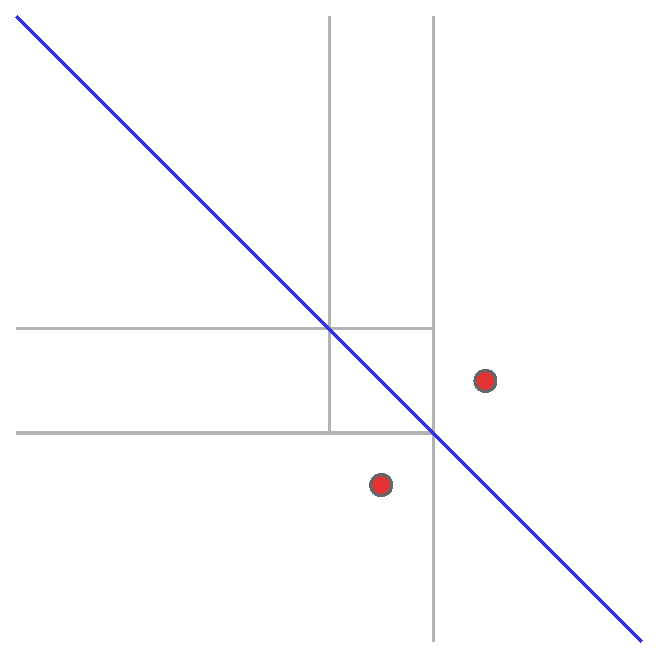
\includegraphics[scale=0.5]{diagrams/no_finite_tree.eps}
\caption{Representing Nearest Neighbour Search with Axis Aligned Hypercubes}
\label{fig:no_finite_tree}
\end{center}
\end{figure}

Because of this limitation, nearest neighbour search in a data structure based
upon orthogonal decomposition can not be done solely by point location. The
algorithm instead is, given a query point, perform point location for that
input point, keeping track of the closest point seen while traversing the tree.
Because the nodes in the tree do not represent the area for which the closest
point is the true nearest neighbour, it is possibly that the true nearest
neighbour is contained in a node which does not contain the query point. To
find the true nearest neighbour, it is necessary to backtrack and examine the
other sibling nodes for each parent node back to the root of the tree, to see
if they in fact contain a point nearest to the query point that the closest
point found so far.

This backtracking process can be more expensive than the initial depth first
search, but can be made much cheaper by doing approximate nearest neighbour
search, where nodes are only visiting during backtracking if they contain a
point which is within an predetermined approximation factor of the distance from
the query point to the current approximate nearest neighbour \cite{app-ann}.
Even with approximation nearest neighbour search, the cost of backtracking
increase as the number of dimensions increases. Empirical evidence suggests that
in problems with 16 dimensions or more, using orthongal decomposition based
approaches performs no better on average than a brute force search of all of the
sites \cite{fastvector}.

Despite these limitations, data structures based upon orthogonal decomposition
are widely used and appear to be the fastest solution in practice for small
dimensional problems. They are relatively simple to implement and avoid
geometric and numerical robustness problems. 

Some non-comparison based approaches include locality sensitive hashing
\cite{lsh} where near by points are hashed to the same cell, or metric trees,
where points are sorted based upon distance to a reference point rather than
based upon their coordinates. Chapter 4 of the book by Samet \cite{samet}
features a comprehensive treatment of nearest neighbour search in higher
dimensions. The paper by Liu et al. evaluates some of these techniques
experimentally \cite{practicalann}. 

We also restrict ourselves to an in-memory model and do not consider external
memory based data structures such as R-trees \cite{rtree}. Since an odds-on tree
is essentially a cache, it is less interesting to consider an external memory
representation, although an odds-on tree may be quite useful as an in-memory
cache for an external memory data structure.

\subsection{General Algorithm for Nearest Neighbour Search}

Nearest neighbour search in data structures based upon orthogonal decomposition
is done according to the same general algorithm, based upon the description for
kd-trees in \cite{samet}. It is described in detail here, rather than being
repeated in the sections describing individual data structures below.

As described above, a data structure based upon orthogonal decomposition of
a $d$ dimensional space is a tree where each node is an axis-aligned box in
$R^d$. It is constructed based upon a set of input nodes, called sites.

Each child node covers a smaller area than its parent node. The root node
covers the area containing all of the input points which were used to construct
the tree. An internal node is a node with at least on child, and an external
node is a node with no children. Depending upon the data structure, every node
may have a site associated with it, or sites may only be associated with
external nodes. If a node is associated with a site, it is contained within the
node's axis aligned box.

Given a query point $p$, nearest neighbour search is performed by a mixture of
depth first search and backtracking. A priority queue, initially containing only
the root node is used for backtracking. The priorities are based upon the
distance from the $p$ to the nearest edge of the axis-aligned box associated
with the node. This backtracking is required due to a finite orthogonal
decomposition being unable to exactly represent nearest neighbour search, as
described above.

A node is first popped from the priority queue and the distance from the query
point to the closest axis is compared to the distance from the query point to
the candidate nearest neighbour. If the closest face of the bounding box is
further away than the candidate nearest neighbour, then all sites contained
within the box associated the node must also be farther away than the candidate
nearest neighbour. Since the priority queue is maintained based upon distance
from the query point, it is not necessary to search the the remaining nodes and
the candidate nearest neighbour is returned as the result to the nearest
neighbour search.

If it is necessary to search the node, depth first search is performed on the
node to locate the external child node containing the query point $p$. For each
child node visited, if there is a site associated with that child, the distance
from the $p$ to that site is calculated and if it is less than the distance to
the candidate nearest neighbour, the site becomes the new candidate nearest
neighbour. The distance to the closest face of the bounding box of any sibling
nodes is calculated and the are added to the priority queue so they can
potentially be visited while backtracking. The depth first search continues
until an external node is visited. At this point, a new node is popped from
the priority queue as described above.

These two cases are illustrated in figure ~\ref{fig:nn_search}. On the left hand
side, the candidate nearest neighbour is further away than the nearest side of
the bounding box for a node and so further search is required. On the right hand
side, the candidate nearest neighbour is closer than the bounding boxes of the
other nodes and so is the true nearest neighbour and the search is finished.

\begin{figure}
\begin{center}
\includegraphics[scale=0.5]{diagrams/nn_search.eps}
\caption{Nearest Neighbour Search Algorithm}
\label{fig:nn_search}
\end{center}
\end{figure}

To extend this algorithm to support \(k\)-nearest neighbour search a priority
queue of candidate nearest neighbours can be maintained rather than using a
single nearest neighbour. For efficiency, the size of the priority queue can be
limited to only hold \(k\) nodes. When a node is popped from the
priority queue, the distance from th \(k\)-th nearest neighbour is compared to
the distance to nearest face of the bounding box \cite{samet}.

This algorithm also supports \(1 + \epsilon\)-approximate nearest-neighbour
search. In this case, when a node is popped from the priority queue, the
distance to the nearest face of the bounding box is multiplied by
\(1 + \epsilon\) prior to comparing it to the candidate nearest neighbour
\cite{samet}.

\subsection{Voronoi Diagrams}

The Voronoi diagram for a set of sites is the subdivision of the plane (or
hyperplane in higher dimensions) into cells, where for every point in a cell,
its nearest neighbour is the site associated with the cell. Given a Voronoi
diagram, nearest neighbour search is a matter of determining in which
subdivision the query point lies.

Efficient algorithms exist for creating Voronoi diagrams in low dimensions:

\begin{thm} \emph{(Voronoi Diagram Construction)}
The Voronoi diagram for a set of $n$ points in two dimensions can be computed
in time \(O(n \log n)\). In higher dimensions, the time becomes
\(O(n \log n + n^{\lceil(d/2)\rceil})\) where $d$ is the dimensionality of the
space \cite{dutch}.
\end{thm}

\begin{figure}
\begin{center}
\includegraphics[scale=0.5]{diagrams/voronoi.eps}
\caption{Voronoi Diagram}
\label{fig:voronoi_diagram}
\end{center}
\end{figure}

\subsubsection{Nearest Neighbour Search in a Voronoi Diagram}

Once the Voronoi diagram is constructed, determining the nearest neighbour can
be done by performing point location to determine in which Voronoi cell the
query point lies.

In 2D, an efficient data structure for the more general problem of point
location in a planar subdivision was described by Kirkpatrick
\cite{kirkpatrick}. It based upon first triangulating the subdivision and then
removing independent vertices (those which do not share an edge) from the
triangulation to create a triangulation with fewer faces. Provided a constant
fraction of constant vertices are removed from the triangulation at each step,
performing the triangulation recursively will result in a data structure that
supports point location in logarithmic time.

\begin{thm} \emph{(Point Location in the Plane)}
A data structure exists using \(O(n)\) storage that allows for planar
point location to be performed in \(O(\log n)\) time \cite{kirkpatrick}.
\end{thm}

The same bounds were achieved using different data structures by Sarnak and
Tarjan \cite{sarnak} and Edelsbrunner et al. \cite{edelsbrunner}.

In higher dimensions, given $n$ hyperplanes, it is possible to solve this problem
by constructing a \(1/r\)-cutting, that is a collection of simplices that
covers the space and is constructed such that each simplex intersects with no
more than \(n/r\) hyperplanes. Chazelle gives a hierarchical construction
procedure for these hyperplanes such that a simplex is eventually fully
contained in one of the cells, that can then be labelled and used to perform
point location \cite{chazelle}.

\begin{thm} \emph{(Point Location in Higher Dimensions)}
A data structure exists using \(O(n^d)\) storage that allows for  
point location in a d-dimensional arrangement of hyperplanes to be performed in
\(O(\log n)\) time \cite{chazelle}.
\end{thm}

Nearest-neighbour search can be performed using Voronoi diagrams and provides
efficient algorithms in the plane. In higher dimensions, the time required to
build a Voronoi diagram and the space required for the point location data
structure both depend upon the dimension of the space in an exponential fashion,
which limits both their theoretical and practical interest for this problem.

\subsection{Quadtrees}

Quadtrees are based upon recursively dividing n-dimensional space into \(2^n\)
equal sized nodes, with each node in the tree keeping pointers to its
children.  In the two dimensional case, this means that space is divided into
four quadrants, hence the name quadtrees. Quadtrees were introduced in 1974 by
Finkel and Bentley \cite{quadtree}. 

\begin{figure}
\begin{center}
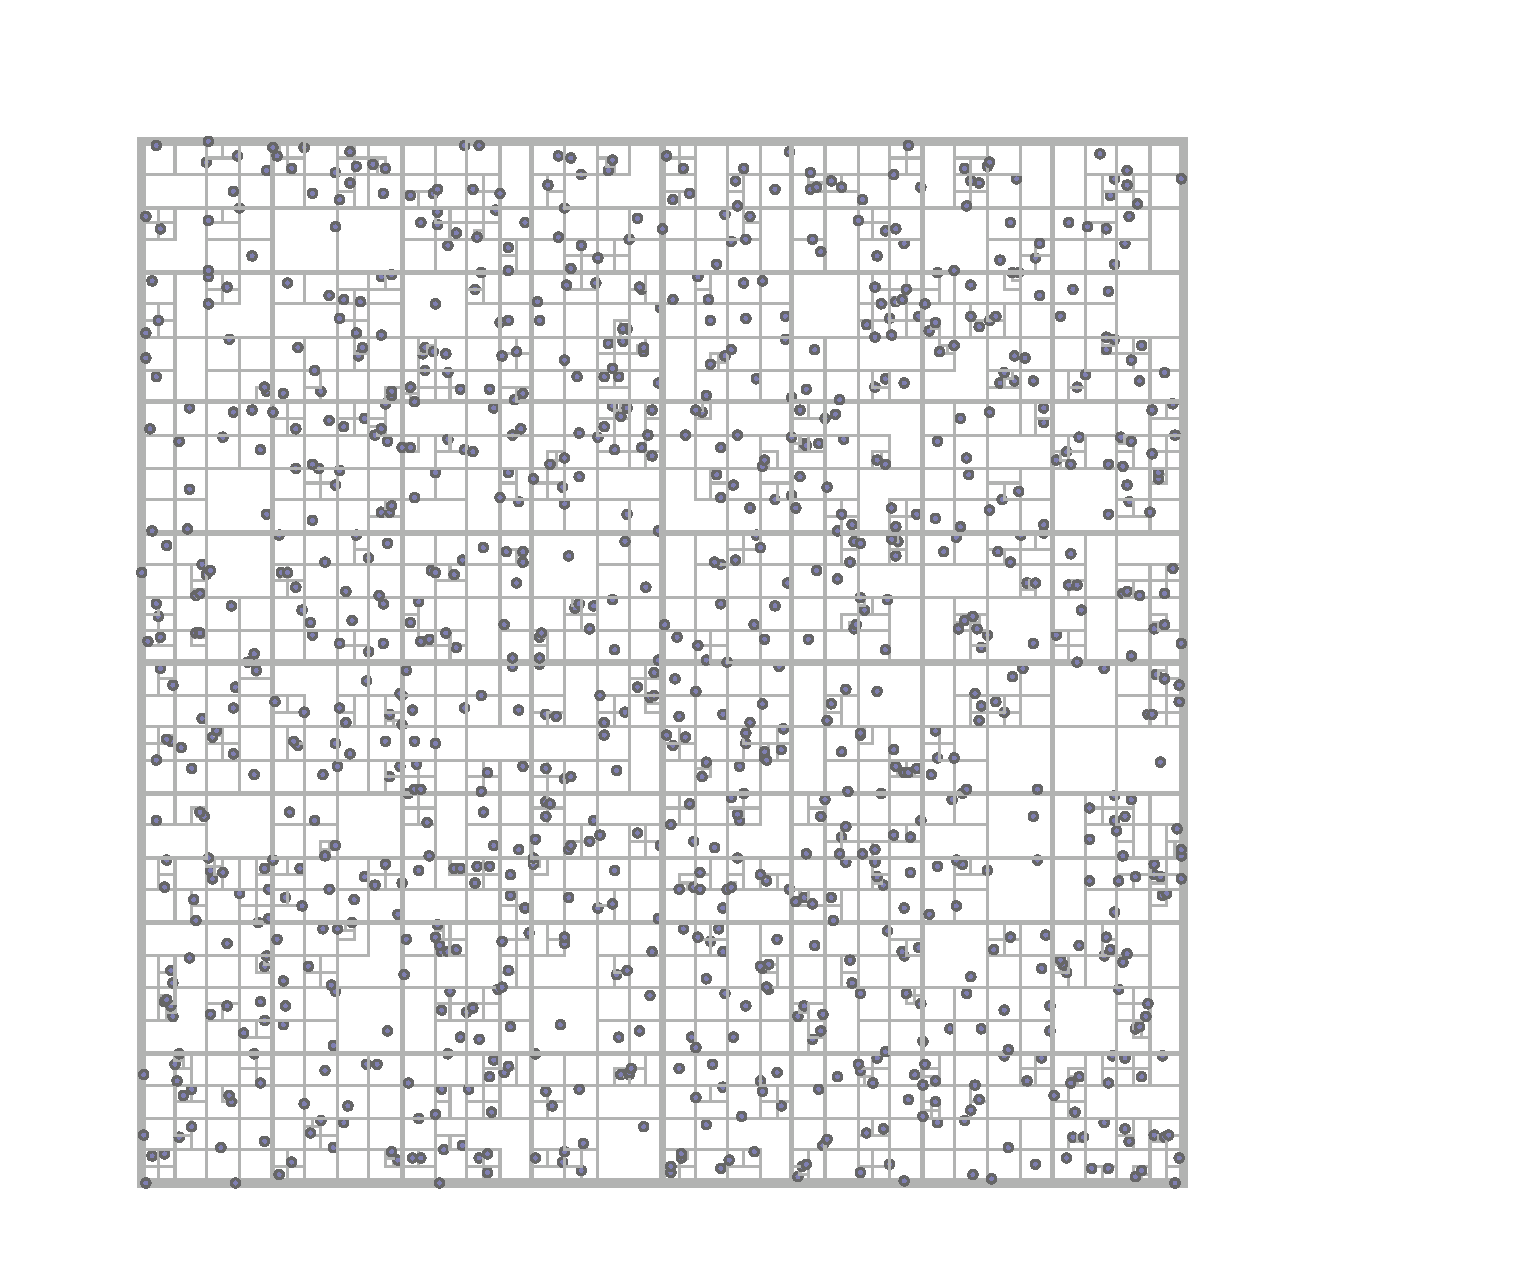
\includegraphics[scale=0.35]{diagrams/quadtree.eps}
\caption{Quadtree}
\label{fig:quadtree}
\end{center}
\end{figure}

Quadtrees can be built over a region, in which case the subdivision proceeds
until the portion of the region covered by a hypercube has the same value for
some property of interest. For example, given an input image, a region based
quadtree would continue to subdivide until each square covered an area that 
had the same colour. Quadtrees over a region are called Trie-based quadtrees in
\cite{samet} and can be used to approximate Voronoi diagrams.

In this section we use quadtrees that are defined over a set of points, in which
case the recursive subdivision is done until each hypercube contains a single
point from the point set.

The root of a quadtree is the hypercube containing all of the points, a leaf
is a hypercube containing a single point, and the height of a quadtree
is the longest path from the root of the quadtree to the leaf of a quadtree
\cite{dutch}.

\begin{thm} \emph{(Height of a Quadtree)}
The height of a quadtree for a set of $n$ points has an upper bound of \(\log(s/c)
+ 3/2\), where c is the smallest distance between any two points in the set, and
s is the side length of the initial hypercube containing all of the points.
\cite{dutch}.
\end{thm}

Note that the height $h$ of the quadtree is not bounded by any function of $n$
and so the running time for algorithms on quadtrees are given in terms of $h$.

\begin{thm} \emph{(Quadtree Construction)}
A quadtree of height h containing $n$ points can be constructed in \(O((h + 1)n)\)
time \cite{dutch}.
\end{thm}

\subsubsection{Point Location in a Quadtree}

Point location in a quadtree is performed by recursively visiting nodes
starting with the root node. At each step, the child node containing the query
point is visited, and the algorithm terminates when a leaf node is reached.

\begin{thm} \emph{(Point Location in a Quadtree)} 
Point location in a quadtree of height h can be performed in time \(O(h)\). 
\end{thm}

\subsubsection{Nearest Neighbour Search in a Quadtree}

Nearest neighbour search in a quadtree is performed as described in the section
on nearest neighbour search in a bounding volume hierarchy.

\begin{thm} \emph{(Nearest Neighbour Search in a Quadtree)} 
Nearest neighbour search in a quadtree of height h requires \(\Omega(h)\) time.
\end{thm}

\subsection{Compressed Quadtrees}

In a compressed quadtree only nodes that contain a point or have at least two
child nodes are present in the tree. Compressed quadtrees were first described
in \cite{compressedquadtree}, and a detailed description can be found in
\cite{skipquadtree}.

A compressed quadtree can be created by pruning nodes from an existing quadtree
as follows:

\begin{enumerate}
\item If a node contains no children and no points, remove it.
\item If a node has a single child node, change the pointer to the node in the
node's parent to point to the node's child.
\end{enumerate}

Because this procedure requires first building a regular quadtree, it also
requires \(\Omega((h + 1)n\) time to complete.

This construction procedure can be made more efficient, or at least bounded by
\(n\), by first sorting the points according to Morton (or z-) order. Morton order
is defined by interleaving the bits of each of coordinate of the point, such
that the first bit of the first coordinate is followed by the first bit of the
second coordinate and so on until one bit has been used from each coordinate.
This is then followed by the second bit of the first coordinate \cite{morton}.
When performed in two dimensions, this results in a z-shaped curve. This
interleaving of bits is called the ``shuffle'' of a point in \cite{bern}.

\begin{figure}
\begin{center}
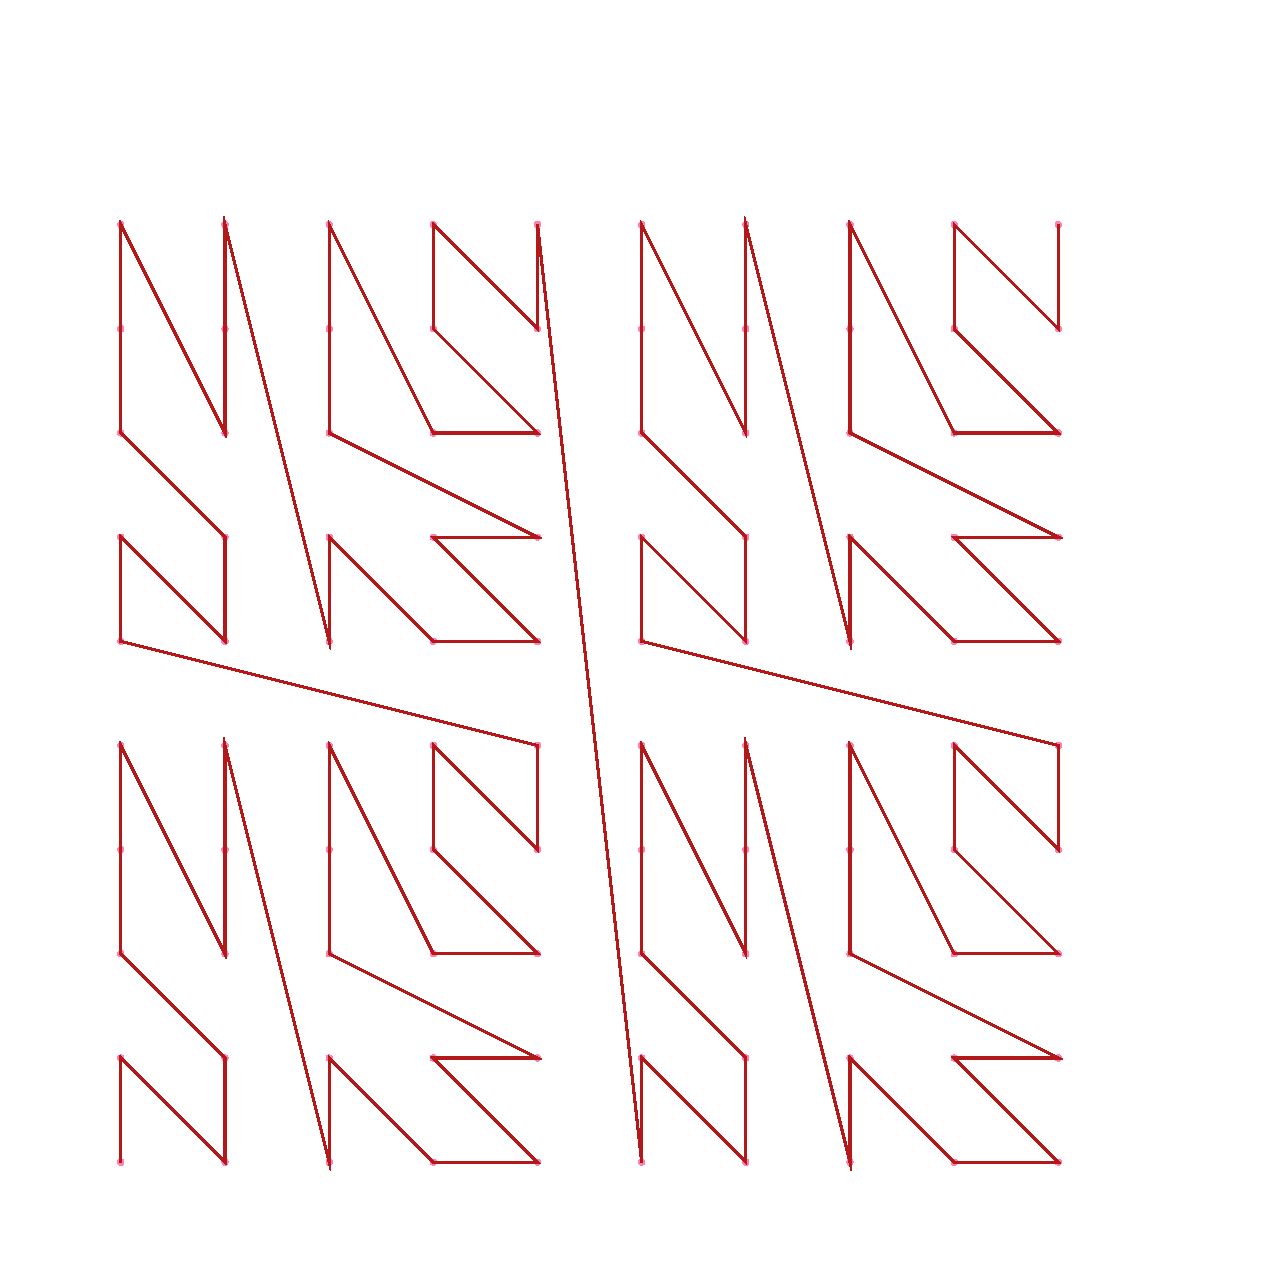
\includegraphics[scale=0.35]{diagrams/zorder.eps}
\caption{Z-Order}
\label{fig:z_order}
\end{center}
\end{figure}

The points are sorted according their Morton order. Each two adjacent points in
the sorted order form a node in the quadtree that can then be nested by finding
the first larger square to the left and the right in the sorted order
\cite{bern}.

\begin{thm} \emph{(Compressed Quadtree Construction)}
A compressed quadtree containing $n$ points can be constructed in
\(O(n \log n)\) time \cite{bern}.
\end{thm}

Chan \cite{chan} showed that the shuffle can be calculated without explicitly
interleaving the bits, and Connor and Kumar \cite{connor} showed that this can
be extended from integer values to IEEE-754 floating point values.

\begin{figure}
\begin{center}
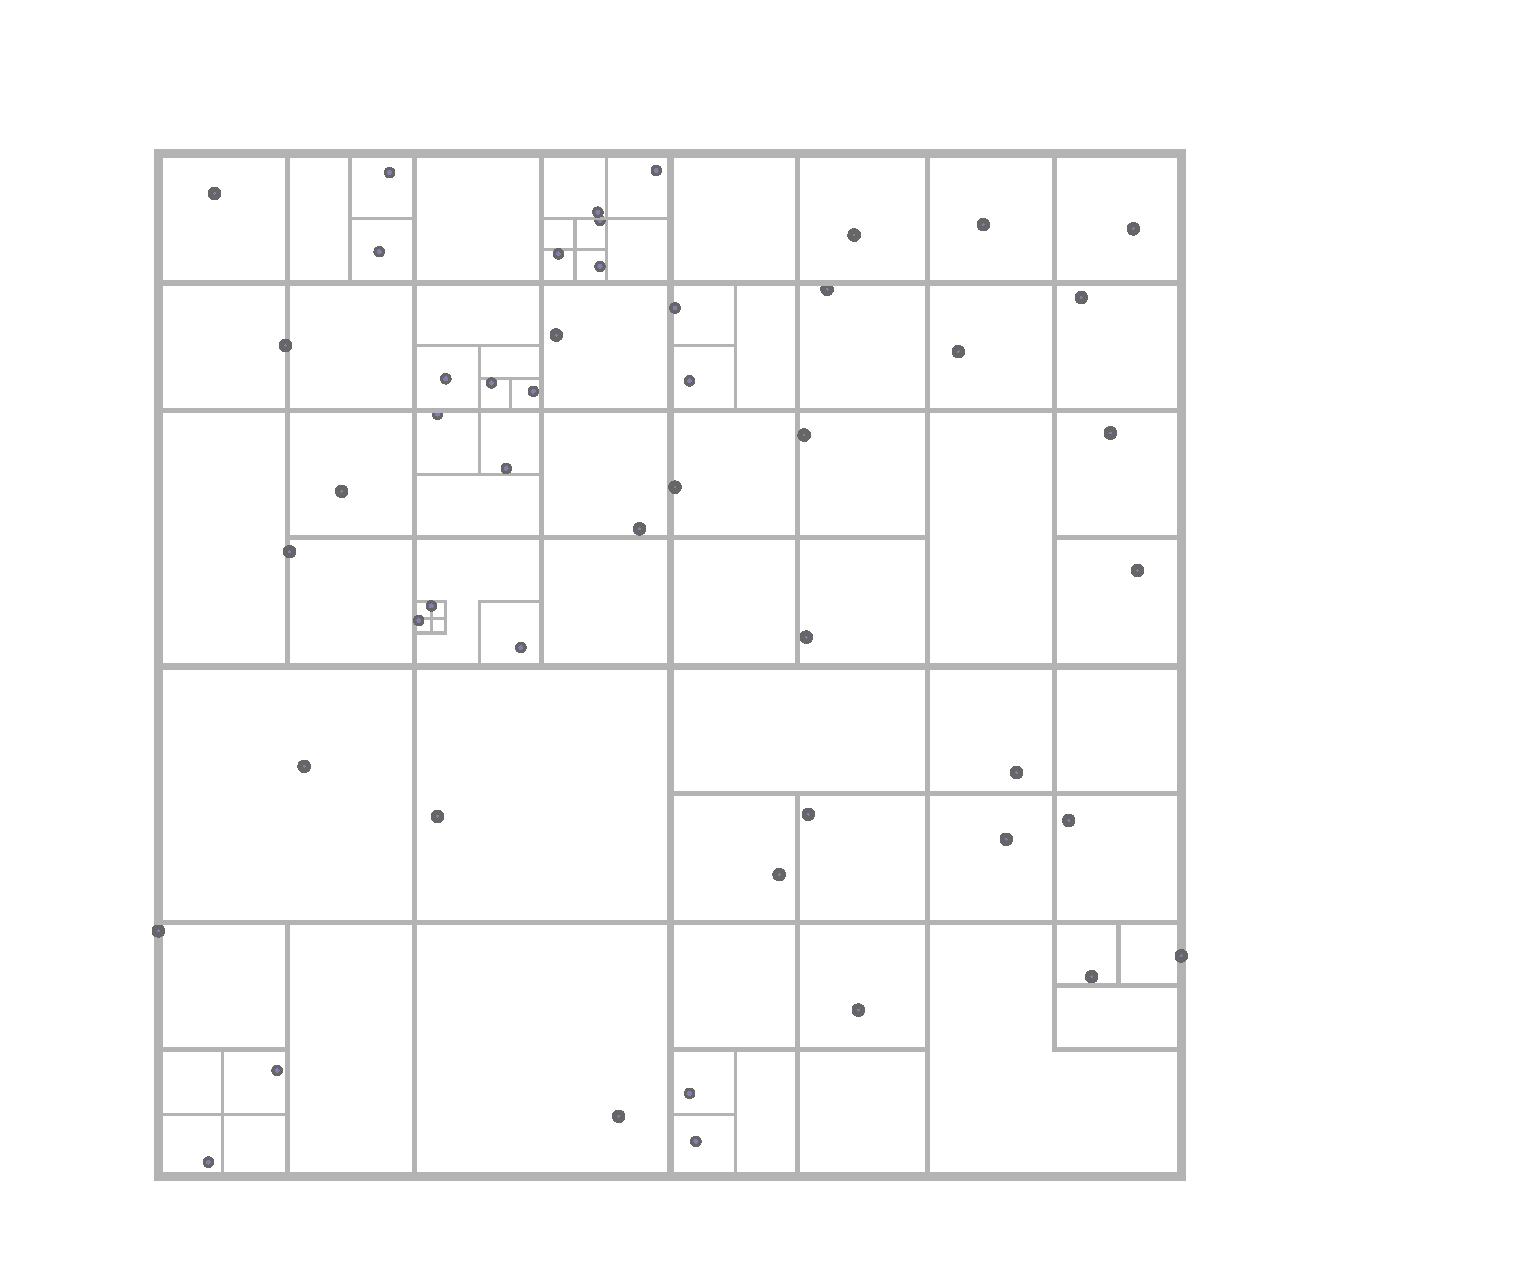
\includegraphics[scale=0.35]{diagrams/compressed_quadtree.eps}
\caption{Compressed Quadtree}
\label{fig:compressed_quadtree}
\end{center}
\end{figure}

\begin{thm} \emph{(Height of Compressed Quadtree)}
The height of a compressed quadtree with $n$ points is \(O(n)\).
\end{thm}

\subsubsection{Point Location in a Compressed Quadtree}

Point location in a compressed quadtree is done by following the same algorithm
as for standard quadtrees. Since the height of a compressed quadtree is
bounded by the number of points, we can bound the time required to perform
point location.

\begin{thm} \emph{(Point Location in a Compressed Quadtree)} 
Point location in a compressed quadtree with $n$ points can be performed in
time \(O(n)\). 
\end{thm}

\subsubsection{Nearest Neighbour Search in a Compressed Quadtree}

Nearest neighbour search in a compressed quadtree can be done by following the
same algorithm as described for bounding volume hierarchies. Again, since the
height of a compressed quadtree is bounded by the number of points, we can bound
the time required to perform point location by a function of $n$.

\begin{thm} \emph{(Nearest Neighbour Search in a Compressed Quadtree)} 
Nearest neighbour search in a compressed quadtree with $n$ points requires
\(O(n)\) time.
\end{thm}

\subsection{Skip Quadtrees}

Skip quadtrees extend the idea of skip lists \cite{skiplist} to two and higher
dimensional spaces. In a skip list multiple levels of linked lists exist, with
pointers between the levels. The bottom level contains all of the nodes, the
top layer is empty, and (in the randomized version of skip lists,) a node
present in a given layer is present in the layer above it with specified
probability. Corresponding nodes on different levels are then linked. The
expected number of layers is logarithmic, allowing for search in \(O(\log n)\)
time.

Skip quadtrees use essentially the same idea, except each level is a
compressed quadtree rather than a linked list, and terminal nodes in the
compressed quadtree at one level are linked to corresponding nodes in the
lower level tree. We summarize the results are for the randomized version of
skip quadtrees. Deterministic results can also be derived using deterministic
skip lists \cite{skipquadtree}.

Since each level of a skip quadtree consists of a compressed quadtree with
approximately half as many points as that in the level below, we expect to
create \(O(\log n)\) compressed quadtrees.

\begin{thm} \emph{(Skip Quadtree Construction)}
A skip quadtree containing $n$ points can be constructed in \(O(n \log^2 n)\)
expected time \cite{skipquadtree}.
\end{thm}

\subsubsection{Point Location in a Skip Quadtree}

Point location in a skip quadtree is performed by recursively visiting each level
of the quadtree. Since each level is a compressed quadtree, point location is
first performed in that compressed quadtree. Once the node in the compressed
quadtree is located, the link to the corresponding node in the lower level
is visited until the bottom level is reached and the node in that compressed
quadtree is returned as the result of the point location query. The expected
amount of work performed in each level is constant \cite{skipquadtree}.

\begin{thm} \emph{(Point Location in a Skip Quadtree)} 
Point location in a skip quadtree with $n$ points can be performed in time
\(O(\log n\)) \cite{skipquadtree}. 
\end{thm}

\subsubsection{Nearest Neighbour Search in a Skip Quadtree}

Nearest neighbour search in a skip quadtree is similar to the procedure for
searching in a standard quadtree, but the skip structure is used to limit
the number of nodes visited.

For a node \(p\) removed from the priority queue, the skip structure is used to
determine the node \(q\) that is the smallest node in the lowest skip level
that is equidistant to the query point. It is then necessary to add nodes along
the path from \(p\) to \(q\) into the priority queue for further searching by
examining nodes that potentially intersect with the radius from the query point
to the candidate nearest neighbour. It is shown in \cite{skipquadtree}
that at most \(O(\log \frac{1}{\epsilon})\) nodes on the path from \(p\) to \(q\)
need to be added to the priority queue.

\begin{thm} \emph{(Nearest Neighbour Search in a Skip Quadtree)} 
Approximate \(1 + \epsilon\) nearest neighbour search for d dimensions in a skip
quadtree with $n$ points requires
\(O(\epsilon^{1 - d}(\log n + \log \epsilon^{-1}))\) expected time.
\end{thm}

\subsection{Kd-Trees}

Kd-trees were developed by Jon Bentley in 1975 as an improvement on quadtrees
\cite{kdtree}. Kd-trees are binary search trees for which each non-leaf node
divides the point set in half using an axis-aligned line.

Kd-trees are constructed by choosing an axis, determining the median value in
the point set for the corresponding coordinate, and dividing the points in two
halves using the median value. The two child nodes are then built by
recursively building kd-trees for each half. In the original paper, Bentley
specifies that the axis to split upon is chosen round robin, level by level,
but it is possible to develop heuristics that potentially give better splits
for specific problems.

\begin{thm} \emph{(Height of a Kd-Tree)}
The height of a kd-tree with $n$ points is \(O(\log n)\).
\end{thm}

\begin{figure}
\begin{center}
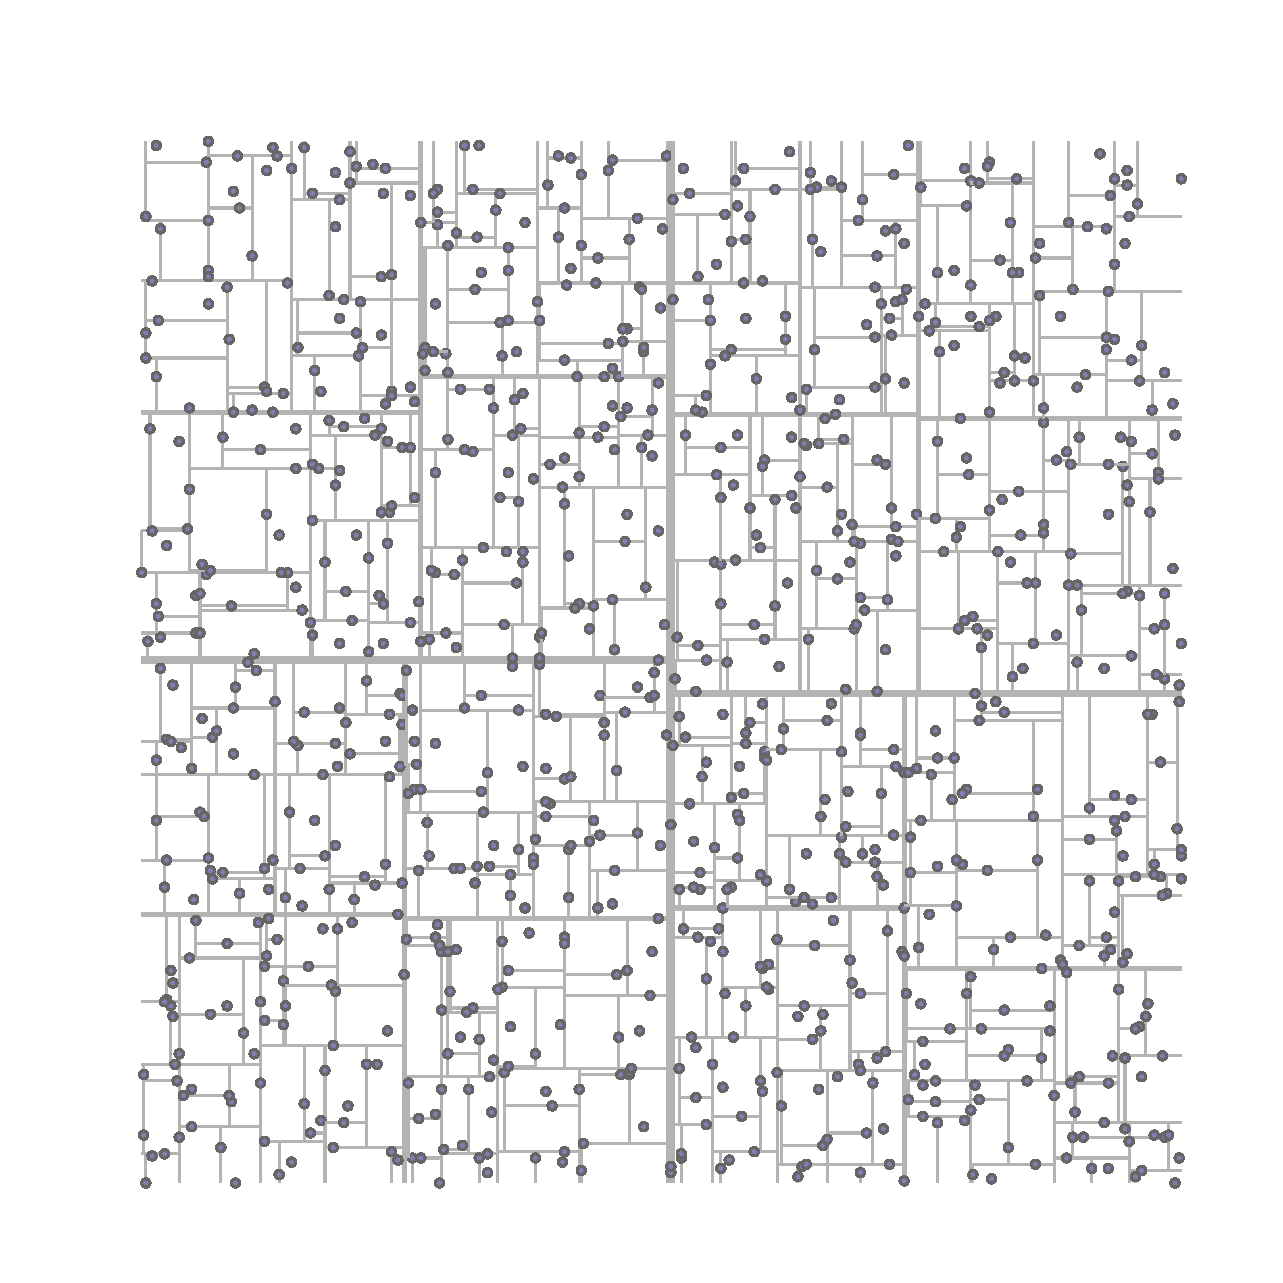
\includegraphics[scale=0.35]{diagrams/kdtree.eps}
\caption{Kd-Tree}
\label{fig:kd_tree}
\end{center}
\end{figure}

\subsubsection{Point Location in a Kd-Tree}

Point location in a kd-tree can be performed by recursively visiting nodes and
comparing the appropriate coordinate of the point to the splitting axis used
to split the children for that node, and the visiting the appropriate child
node \cite{kdtree}.

\begin{thm} \emph{(Point Location in a Kd-Tree)} 
Point location in a kd-tree with $n$ points can be performed in time
\(O(\log n\)). 
\end{thm}

\subsubsection{Nearest Neighbour Search in a Kd-tree}

Nearest neighbour search in a compressed quadtree can be done by following the
same algorithm as described for bounding volume hierarchies.

\begin{thm} \emph{(Nearest Neighbour Search in a Kd-tree)} 
The expected time for nearest-neighbour search in a kd-tree with $n$ points is
\(O \log(n)\), and the worst case is \(O(n)\) \cite{friedman}.
\end{thm}

\subsection{Balanced Box Decomposition (BBD) Trees}

A balanced box decomposition tree is a data structure invented by Arya et al.
\cite{optimalann} that combines advantages of both quadtrees and kd-trees.
Like a kd-tree, as one traverses the tree, the number of points associated with
a node decreases exponentially, and like a quadtree, the area associated with a
node also decreases exponentially. By combining these properties, an optimal
data structure for approximate nearest neighbour search is obtained.

Each node in a BBD-tree covers a cell that is the set theoretic difference
between an outer box and an optional inner box. Both boxes are axis-aligned.
If present, the inner box must either touch the edge of the outer box, or be
separated from each edge by at least the width of the box in the direction of
the edge, in which case the node is called ``sticky''. Figure
~\ref{fig:bbd_tree_node} reproduced from \cite{optimalann} illustrates
``sticky'' and ``non-sticky'' nodes. Each node is an BBD-tree has a bounded
aspect ratio that ensures that the ratio of the shortest edge to the longest
edge is bounded by some constant.

A BBD-tree is constructed through a sequence of two operations, fair-splits
and shrinks. A fair-split is a partition of a box using an axis aligned
hyperplane that maintains the aspect ratio bound but does not necessarily
result in an even partition of points. A shrink operation divides a node into
inner and outer boxes that is used in a manner similar to a compressed
quadtree and can ensure an even partition of points \cite{optimalann}.

Both fair-splits and shrinks can be performed in time linear in the number of
points contained in the cell. A simple strategy for partitioning the points is
the midpoint algorithm that performs a fair-split by partitioning the node
with a hyperplane orthogonal to the longest edge of the outer box. A shrink
operation is somewhat more complicated, potentially requiring two shrink nodes
and one split node to ensure that no child contains more than \(2/3\) of the
points covered by the parent node \cite{optimalann}.

To prove properties of the BBD-tree, Arya et al. assume that fair-splits and
shrinks are applied alternately as the tree is constructed. In practice, they
note that for almost all cases only fair-splits are required \cite{optimalann}. 

\begin{thm} \emph{(BBD-Tree Construction)} 
A BBD-tree for a \(d\)-dimensional space has \(O(n)\) nodes and can be build in
\(O(d n \log n)\) time \cite{optimalann}.
\end{thm}

\subsubsection{Nearest Neighbour Search in a BBD Tree}

Nearest neighbour search in a BBD Tree is performed in a manner similar to
search in a kd-tree. A priority queue is maintained of nodes to visit that 
initially contains the root node. At each step of the search, the closest
node to the point is removed from the queue and is recursively searched for
the leaf closest to the search point. The distance to the other child nodes
encountered in the search is calculated and they are enqueued in the priority
queue. The search continues until the distance to the node at the top of the
priority queue exceeds the distance to the candidate nearest neighbour. This
can be easily extended to find k nearest neighbours, and to find approximate
nearest neighbours rather than an exact ones.

\begin{thm} \emph{(Nearest Neighbour Search in a BBD Tree)} 
Given a constant \(c_{d,\epsilon} \le \lceil 1 + {6d \over \epsilon} \rceil^d\)
where d is the dimensionality of the space and \(\epsilon\) is the approximation
factor, a \((1 + \epsilon)\)-nearest neighbour search in a BBD Tree can be
performed in time \(O(c_{d,\epsilon} \log n)\) time and k approximate nearest
neighbours can be found in \(O((c_{d,\epsilon} + kd) \log n)\) time.
\end{thm}

\subsection{Approximate Voronoi Diagrams}

For approximate nearest-neighbour searches, it is possible to improve on the
space requirements by creating an approximation to the Voronoi diagram, for
instance using quadtrees \cite{avd}. The complexity of the calculation is
reduced by constructing the Voronoi diagram such that for each cell, any point
within it is a \(1 + \epsilon\)-nearest neighbour, rather than an exact
nearest neighbour.

Har-Peled \cite{avd} provides an algorithm for building an approximate
Voronoi diagram that supports nearest-neighbour searches. His construction is
complicated, requiring first clustering the input sites, then
building a data structure for answering point location in equal ball queries
(a technique also used in locality sensitive hashing \cite{lsh}) and finally
using this data structure to build the approximate Voronoi diagram using
compressed quadtrees.

Arya et al. \cite{arya-avd} extend this to \(t, \epsilon\)-AVD where each
cell in the approximate Voronoi diagram stores \(t\) approximate nearest
neighbours. Their construction makes use of a well-separated pair
decomposition of the sites of the Voronoi diagram. Two sets of points are well
separated if each set can be bounded by a ball of radius \(r\) such that the
distance between the center of each set is at least \(2r\). By decomposing
the sites into well-separated subsets, a set of quadtree nodes can be
generated that are then stored in a BBD-tree. 

We do not describe the construction algorithm in detail as these results are
not used in the remainder of the thesis because we only consider exact
nearest neighbour search. We note that both \(\epsilon\) and t need to be fixed
at construction time, which is less flexible than using quadtrees or kd-trees
directly.

\begin{thm} \emph{(Nearest Neighbour Search in a Approximate Voronoi Diagram)} 
An approximate Voronoi diagram of size \(O({n \over \epsilon ^ d})\) can be
constructed that can answer \((1 + \epsilon)\) approximate nearest neighbour
searches in time \(O(\log {n \over \epsilon})\) \cite{arya-avd}.
\end{thm}

\section{Biased Search}

Biased search is a generalization of search where rather than assuming each
search result is equally likely, instead a probability distribution over the
results is available.

We begin by describing some results from information theory that provide a
bound on how well a biased data structure can perform. We then describe some
classical results for biased search in a single dimension, and then proceed
to some more recent results for higher dimensional search.

\subsection{Information Theory}

Lower bounds for search depend upon some results from information theory that
are briefly summarized here. Information theory is the study of the fundamental
properties of communication systems. A data structure can be seen as a form of
communication system because it provides a means of communicating data from the
present to the future. A data structure that allows for efficient search is
essentially solving the same problem as creating an efficient code with which
to transmit a message. The message here is the result of the search.

Based upon earlier work by Ralph Hartley, Claude Shannon \cite{claudeshannonwasagod}
defined entropy as the measure (in bits) of the amount of randomness of a set.
That is if \(p_i\) is the probability of the \(i\)-th member of the set, then the
entropy \(H\) is defined as
$$
H = \sum{ p_i \log{1 \over p_i}}
$$

Shannon also proved that the efficiency of any communication system is limited
by the entropy of the set of messages to be transmitted.

\begin{thm} \emph{(Fundamental Theorem for a Noiseless Channel)} 
Given a source with entropy \(H\) (in bits) and a channel with capacity \(C\)
(in bits per second), then it is possible to encode a source in such a way as to
transmit at an average rate of \({C \over H} - \epsilon\) symbols per second
where \(\epsilon\) is arbitrarily small, and it is not possible to transmit
at an average rate greater than \(C \over H\) \cite{claudeshannonwasagod}.
\end{thm}

To see how a data structure can be viewed as a communication system consider 
querying a binary search tree for a set of keys. If at each node, a ``0'' or
``1'' is generated depending upon whether the left or right subtree is taken,
then the generated sequence is a code for the key, and we can apply Shannon's
theorem to give a bound on the expected number of comparisons required.

For random queries for which the data structure has no information other than
the distribution of outcomes, so that \(p_i\) is the probability of retrieving
the \(i\)-th key, then any data structure for search can not have an expected
number of comparisons less than \(H\).

Since search time depends upon the expected number of comparisons, the expected
search time is bounded by the entropy and \(\Omega(H)\) is a lower bound on
the search time for any data structure.

\subsection{Biased Search Trees}

A biased search tree is a generalization of binary search trees that make use
of knowledge of the probability distribution of the search keys to balance the
tree.

The initial work on biased search trees focused on the static case, where
the query frequencies are known in advance and no deletions and insertions of
keys are allowed. This work is summarized in Volume 3 of Donald Knuth's The Art
of Computer Programming \cite{knuth}.

Given a set of $n$ keys \(K_i\) and \(2n + 1\) probabilities
\(p_1, p_2, ..., p_n\) and \(q_0, q_1, ..., q_n\) where \(p_i\) is the
probability that \(K_i\) is the search item and \(q_i\) is the
probability that the search item lies between \(K_i\) and \(K_{i+1}\), an
optimal biased search tree is one that minimizes the expected number of
comparisons to search the tree \cite{knuth}. %TODO: check this

Each subtree of a optimal biased search tree is itself optimal, and so the
problem can be solved through a dynamic programming algorithm, using the
following relation: Define \( c(i,j)\) as the cost of an optimum subtree with
weights \((p_{i+1}, ..., p_j; q_{i+1}, ..., q_j;)\) and \(w(i, j)\) be the
sum of the weights, i.e. \(p_{i+1} + ... + p_j + q_{i + 1} + ... + q_j \)
\cite{knuth}.

Then we have that:

\begin{equation}
    \begin{aligned}
    c(i, i) & = 0 \\
    c(i, j) & = w(i, j) + \min_{1<k<j} (c(i, k - 1) + c(k, j)), \text{for } i<j, \\
    \end{aligned}
\end{equation}

This recurrence allows us to find all optimal one node trees and then use those
to find all optimal two node trees, and so forth, until an optimal search
tree has been determined. This minimization is applied to \({1\over{6}} n^{3} \)
values of \( k \), but a monotonicity property allows the running time to be
reduced to \( O(n^2) \) \cite{knuth}.

\begin{thm} \emph{(Construction of an Optimal Static Biased Binary Search Tree)} 
An optimal static biased search tree can be constructed in time \(O(n^2)\) and
space \(O(n^2)\) using dynamic programming \cite{knuth}.
\end{thm}

Knuth also proposed two heuristics that run in \(O(n \log n)\) time and
\(O(n)\) space that produce nearly optimal trees:

Rule I: Use the most frequent item as the root of the tree and apply the same
rule to the subtrees.

Rule II: Choose as the root the item that results in the weight of the left
and right subtrees being as close to equal as possible and apply the same
rule to the subtrees. 

Mehlhorn \cite{mehlhorn} analyzed the results of applying these two rules. He
provides a simple example where Rule I will produce a tree with expected
search time \(\Theta(n)\).

His analysis of Rule II shows that the expected search time for item in the tree
is bounded from above by the entropy \(H\) of the query frequency distribution.
If $P_{opt}$ is the weighted path length of an optimum search tree, and
$P_{balanced}$ the weighted path length of a balanced search tree constructed
according to Rule II, then

$$
{\log(3)}^{-1} \cdot H \le P_{opt} \le P_{balanced} \le 2 + {(1 - \log(\sqrt 5 - 1))}^{-1} \cdot H
$$

\begin{thm} \emph{(Nearly Optimal Static Biased Binary Search Tree)} 
A static biased search tree where the search time for an item is bounded by
the entropy \(H\) of the frequency distribution can be constructed in time
\(O(n \log n)\) and space \(O(n)\) \cite{mehlhorn}.
\end{thm}

Biased search trees allowing insertions and deletions based upon 2-4 and
red-black trees were described by Bent, Sleator and Tarjan \cite{bst} in 1984.
As with 2-4 trees, their data structure relies upon maintaining invariants
on the tree during updates through extensive multi-case rules for re-parenting
nodes to maintain balance. In this case, the balance condition depends upon the
weight of the node, where the weight can be set based upon the probability of
its retrieval. If all of the weights are one, the resulting tree is simply a 2-4
tree. Somewhat simpler trees are provided by Feigenbaum and Tarjan \cite{bst2}.
The construction of both data structures requires the consideration of a large
number of subcases to maintain balance and so we do not describe them further
here.

\begin{thm} \emph{(Construction of a Dynamic Biased Binary Search Tree)} 
A dynamic biased search tree can be constructed in time \(O(n)\) that can
perform searches in time \(O(\log(w))\) where \(w\) is the weight of the item
searched for and insertions and deletions in amortized time \(O(W / w)\)
where \(W\) is the total weight of all items in the search tree and \(w\) is
the weight of the item added or removed \cite{bst2}.
\end{thm}

\subsection{Splay Trees}

An alternative approach to biased search is to use data structures that 
modify themselves in response to queries rather than insertions or deletions. In
this case, rather than specifying the probabilities in advance, the data
structure will change itself to match the query distribution. 

Splay trees, which were invented by Sleator and Tarjan \cite{splaytree}, are a
self-modifying binary search tree that perform well in practice. They operate
by moving the most recently accessed node to the root of the tree using a
process called splaying that rotates items in pairs according to three cases
that depend upon the structure of the tree.

Although splaying can be costly for an individual access, in an amortized
sense, operations on a splay tree take \(O(\log n)\) time.

\begin{thm} \emph{(Splay Trees)} 
Insertion, deletion and search in a splay tree take \(O(\log n)\) time in
an amortized sense \cite{splaytree}.
\end{thm}

Sleator and Tarjan also showed that splay trees perform within a constant
factor of any static optimal search tree over a sequence of accesses, and
famously, conjectured that splay trees also perform within a constant factor
of any dynamic search tree as well.

\begin{thm} \emph{(Static Optimality of Splay Trees)} 
The total amortized time required for a sequence of $m$ accesses to a $n$
node splay tree is \(O(n \log n + mH)\) \cite{splaytree}.
\end{thm}

It is possible to create biased versions of other, simpler data structures
such as randomized search trees (treaps) \cite{treap} and skip lists
\cite{bsl2} but these do not provide better theoretical performance guarantees
than biased search trees and also do not seem to provide better performance in
practice than splay trees.

\subsection{Planar Point Location}

Looking at biased search in higher dimensions, we first consider the planar
point location problem: given a subdivision of the plane and a query point \(p\),
construct a data structure that allows us to efficiently determine which face
of the plane contains \(p\). If all of the planar subdivisions and the query
point lie on a single line then this problem is the standard one dimensional
search problem and the appropriate data structure is a binary search tree.

We discussed the non-biased version of this problem above in the section on
nearest-neighbour search in a Voronoi diagram, and noted that a linear space
and \(O(\log n)\) search time solution existed for this problem.

In the biased case, as with binary search trees, if \(p_i\) is the probability
that the answer to a query is in the \(i\)th face and we are given a probability
distribution over the faces such that each is chosen with \(p_i\) then the
expected number of comparisons required to locate the query point \(p\) is
lower bounded by the entropy of the set of faces.

A data structure for biased point location in a triangulation was described
by Iacono \cite{iacono}. It is based on a variation of Kirkpatrick's data
structure for solving point location \cite{kirkpatrick}, which works by
constructed a hierarchical triangulation by selectively removing vertices
from each level of the hierarchy, until the top level contains a single triangle.

In Iacono's version, the vertices chosen to be removed are such that they are
not of large degree and are not incident to a high probability region. Another
approach, by Arya et al. matches these space and time bounds \cite{simpleentropy}.

\begin{thm} \emph{(Distribution Sensitive Point Location in a Triangulation)} 
Given a triangulation, it is possible to perform point location in time
\(O(H + 1)\) and space \(O(n)\) where H is the entropy of the set of triangles
making up the triangulation. 
\end{thm}

\subsection{Biased Range Trees}

Biased range trees are a data structure invented by Dujmovic et al.
\cite{biasedrange} to solve two-sided planar orthogonal range counting problems.
Given a set \(S\) and a query point \(q_x, q_y\), the problem is to count all
points in \(S\) that are above and to the left of the query point
\(q_x, q_y\), that is \(p_x \ge q_x\) and \(p_y \ge q_y\). Although the biased
range tree solves a fairly restricted problem, it shares many ideas with odds-on
trees and is worth considering in detail.

This is a restricted case of the orthogonal range counting problem that allows
for a rectangular query area in two or higher dimensions. A data structure
invented by Jon Bentley \cite{rangetree} called a Range Tree can solve range
search problems in linear space and logarithmic time. A one dimensional range
tree is simply a balanced binary search tree, and in \(d\) dimensions, one
coordinate is chosen to create a binary search tree, and each child node
contains a \(d - 1\) range tree. 

\begin{thm} \emph{(Planar Range Search using Range Trees)} 
A range tree for a set of points \(S\) of cardinality \(n\) can be built in
time \(O(n \log n)\) and requires \(O(n \log n)\) space. It can report the
points in a rectangular query area in time \(O(\log^2 n + k)\) time, where
\(k\) is the number of points in the query area. Using fractional cascading can
reduce the query time to \(O(\log n + k)\) \cite{dutch}. 
\end{thm}

Kd-Trees and quadtrees can also be used to solve the orthogonal range counting
problem, but with \(O(\sqrt n)\) time and \(O(n)\) worst case query time
respectively \cite{dutch}.

The answer to any range counting query is an integer in \({0, ..., n}\). Let
\(p_i\) be the probability that the answer is i. Since we are operating in a
comparison based model, Shannon's theorem for a noiseless channel applies and
the entropy \(H=\sum_{i=0}^n{p_i\log(1/p_i)}\) is a lower-bound on the number of
comparisons required. This is not a tight lower bound, and no comparison (or
decision) tree is able to meet it in general \cite{biasedrange}.

A stronger lower bound for the range counting problem can be found by creating
an arrangement \(A\) of \(2n\) rays originating at each point in the set \(S\),
with one ray facing to the left and one ray facing down. This partitions the
plane into a set of faces \(F(A)\).

Now consider a comparison tree to solve the range counting problem. Each leaf of
the comparison tree is a rectangle because it is based upon comparisons to
coordinates that are axis aligned.  These leaf rectangles do not intersect with
any of the edges of \(A\) because that implies that the answer to the range
counting problem would not be consistent for the entire rectangle. This implies
that we can use \(F(A)\) as a data structure for the range counting problem,
and that Shannon's theorem once again provides a lower bound of:

$$
H=\sum_{f \in F(A)}{p_f\log(1/p_f)}
$$

This lower bound is still not strong enough. To see this consider figure
~\ref{fig:rangelb}. The query points are evenly distributed in the \(n + 1\)
red circles. In this case, the query points are always in the same face of
\(F(A)\), so the entropy above is 0. A comparison tree based data structure
for this problem uses \(n + 1\) leaves to determine which circle contains
the query point, so the the lower bound must be greater than \(\log(n + 1)\).

\begin{figure}
\begin{center}
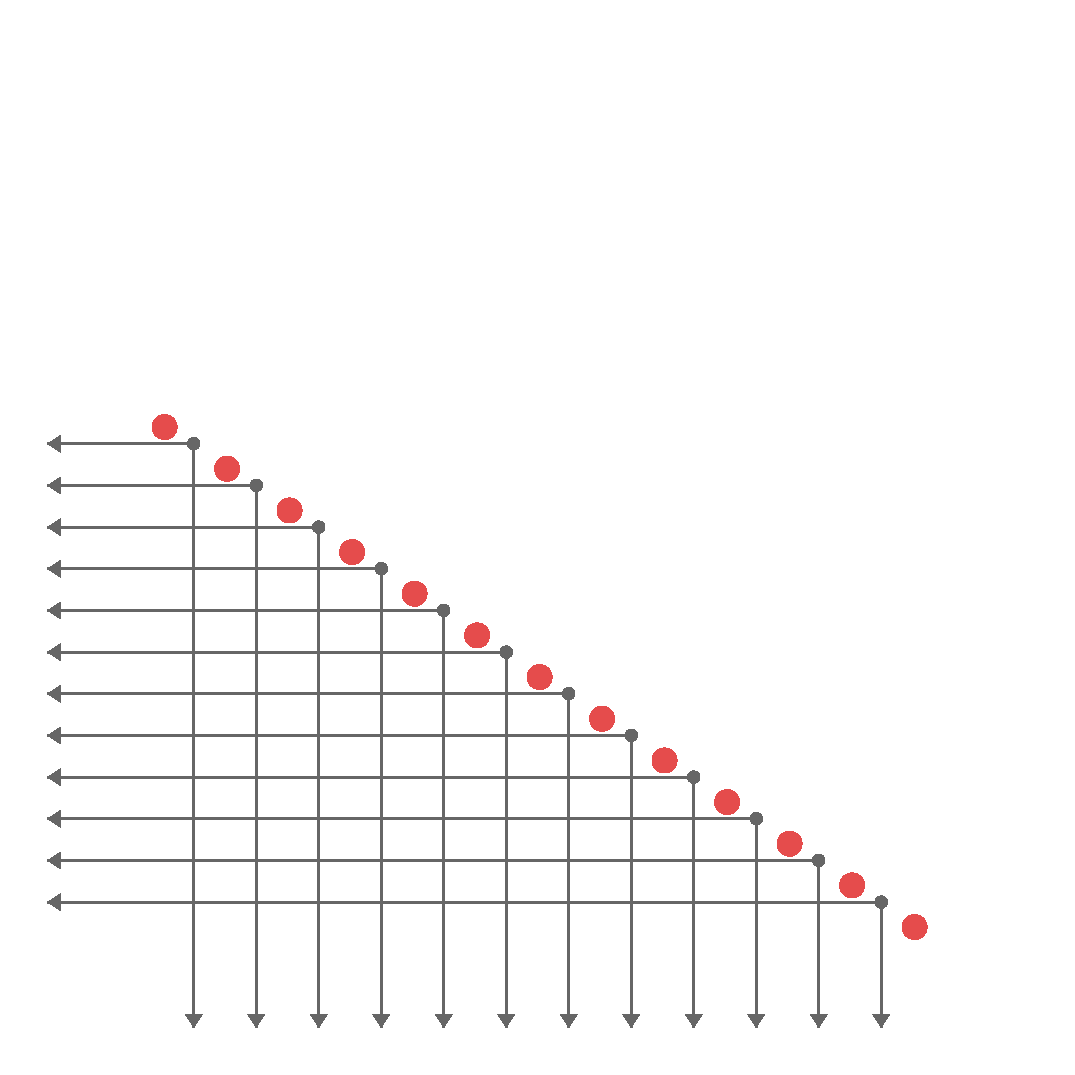
\includegraphics[scale=0.6]{diagrams/range_counting.eps}
\caption{The range counting lower bound is not always achievable}
\label{fig:rangelb}
\end{center}
\end{figure}

A Biased Range Tree relies upon two data structures. The primary search tree
is based upon a kd-tree. The nodes of the primary tree are associated with
regions of space, and the root node covers the plane. Any node in the primary
search tree that has depth greater than \(O(\log n)\) is called a ``bad'' node.
These regions are potentially open on two sides, since the data structure is
designed to support 2-sided queries \cite{biasedrange}. 

Each child node in the tree is constructed by removing a horizontal (at even
depths) or vertical (at odd depths) strip from region associated with the
parent region. These strips are constructed such that the probability a point
being in the region associated with a child node is at most half the probability
of the point being in the parent region.

Each node also has two associated data structures, called catalogues, that 
contain subsets of \(S\) sorted by the x- and y- coordinates respectively.
Each catalogue is indexed by a biased search tree, and fractional cascading is
used to speed up search within the catalogues.

The second data structure is a backup range tree, as described above, that 
uses \(O(n \log n)\) space and can answer range search queries in time
\(O(\log n)\). This data structure is used to answer queries for which the
depth of corresponding node in the primary tree would exceed \(O(\log n)\),
that is the ``bad'' nodes.

Search within the biased range tree occurs as follows: the primary tree is
first searched to find a node such that the query region defined by \(q_x\) and
\(q_y\) is contained within the region corresponding to the node. If this node
is a ``bad'' node, then the backup range tree is used to answer the query.
Otherwise, the indices are used to locate the node are used to locate \(q_x\)
and \(q_y\) in the catalogues for the node determine the result of the range
counting query, and the tree is walked back to the root, locating the query
point in the catalogues of each node along the way, and adding results to
the range counting query.

\begin{thm} \emph{(Two-Sided Orthogonal Biased Range Search)} 
Two sided orthogonal biased range search can be performed using space
\(O(\log n)\) and expected time \(O(H)\) where \(H\) is a lower bound on the
expected number of comparisons done by any comparison-based data structure, so
biased range trees are an optimal data structure for two-sided orthogonal
range search \cite{biasedrange}.
\end{thm}

%TODO: ADDRESSED COMMENTS TO HERE

\subsection{Odds-on Trees}

Odds-on trees make use of similar ideas of those described above to solve
2-sided orthogonal range searches, but are capable of solving a much larger
class of geometric search problems.

Given a probability distribution \(D\) over a set of queries, the odds-on tree
is capable of answering any query drawn from \(D\) in expected time
\(O(H^* + 1)\) where \(H^*\) is a lower bound on the expected cost of any
linear decision tree that solves the search problem. In particular, the
entropy \(H\) of the output \(D\) is one such bound for many search
problems. A linear decision tree is a search tree where the decision of which
child node to follow is based on a linear function.

An Odds-on tree consists of a primary search tree and a backup search tree.
The primary search tree is based upon a data structure called partition trees,
which are an means of dividing \(d\)-dimensional spaces into simplices. A
simplex is the intersection of at most \(d + 1\) halfspaces; a triangle is an
example of a simplex in two dimensions. The simplices in the partition tree
potentially overlap each other.

\begin{thm} \emph{(Partition Trees)} 
Given a set of \(S\) points, for any \(\epsilon > 0\) a data structure called
a partition tree can be constructed that uses \(O(n)\) storage and can answer
counting queries for a search simplex in time \(O(n^{1/2 + \epsilon})\) time and
report those points in an additional \(O(k)\) time, where \(k\) is the number
of points in the search simplex. A partition tree can be constructed in
\(O(n^{1 + \epsilon})\) time \cite{dutch}.
\end{thm}

The points used to create this partition are drawn from the query distribution
\(D\), and the maximum depth of any node in the tree does not exceed a specified
constant. For each node in the partition tree the area corresponding to the node
is searched to see if the answer to the search problem is the same for all points
associated with the area. Since the simplices created by a partition tree are
possibly overlapping, it is necessary to determine the polytope associated with
the node which is not associated with any other node in the tree.

If the result of the search is the same for all points in the polytope, the node
is marked as terminal, any children nodes are removed, and the result of the
search is stored with the node to answer future searches.

The backup tree can be any data structure capable of answering the original
search problem in \(O(\log n)\) time.

Search in the tree occurs as follows. Given a query, the tree is searched until
either a terminal leaf node is reached, in which case the stored result is used
to answer a query, or a non-terminal leaf node is reached, in which case the
backup tree is used to answer the query \cite{oddson}. Essentially the same data
structure with a different analysis was created by Chan et al. \cite{chan}.

\begin{thm} \emph{(Odds-on Tree)}
For any \(n\) and \(\tau>0\) an odds-on tree of size \(m = n^\tau\) of maximum
depth k = \(\lfloor {1 \over 4} \log_{r \over 3} m \rfloor \), where \(r\) is
the number of simplices associated with the root node of the odds-on tree, can
be constructed in time \(O(m \log^{O(1)} n)\) plus the cost of \(O(m)\) samples
from \(D\) plus the cost of \(O(m \log^{O(1)} n)\) searches to determine whether
a node is terminal.

The odds-on tree can be answer searches in expected time \(O(H^* + 1)\) where
\(H^*\) is a lower bound on the expected cost of any linear decision tree
that answers the search \cite{oddson}.  
\end{thm}

\chapter{Implementation}

This chapter describes the implementation of an odds-on tree based data
structure for nearest-neighbour search.

Partition trees were used in the analysis of odds-on trees. Although they have
useful theoretical properties, they are complicated and to our knowledge have
never been implemented and so were not considered as the basis of a practical
implementation.

Compressed quadtrees and kd-trees lack strong theoretical performance
guarantees but they are simple to implement and perform well in practice. In
general, kd-trees have better performance guarantees and out-perform quadtrees,
but we chose to implement both data structures, as the initial results using
kd-trees were not promising and it was possible that quadtrees would have
advantages as the basis for an odds-on tree implementation that outweigh their
disadvantages in general. 

The implementations are in C++. The use of C++ provides great control over
memory allocations and the placement of objects in memory, allowing for
optimizations. Since it is not garbage collected, experimental results are less 
variable as the programs will not be interrupted at unpredictable intervals for
garbage collection. C++ also has reasonably performant implementations of basic
data structures such as vectors and lists in the standard library.

The implementations are parameterized using templates to allow for user defined
classes to be used for points, and the underlying data type used for numbers to
be chosen. The experiments are done using double precision floating point
numbers.

The heap data structure implementation in the C++ standard library on the
development platform was found to have poor performance. Two priority queue
implementation were developed based upon the heap data structure, one of which
enforced a queue size limitation for use when searching for \(k\) nearest
neighbours. Both were found to outperform the C++ priority queue implementation
based upon the std::vector class and were used in the kd-tree and compressed
quadtree implementations.

\section{Kd-tree Implementation}

We first describe our implementation of kd-trees. The kd-tree implementation was
used as the backup oracle for both the kd-tree and quadtree based odds-on tree,
and as the reference implementation of kd-trees for experimentation.

The kd-tree is built as described in chapter two, by choosing a splitting axis
round robin, determining the median value in the point set for the corresponding
coordinate and dividing the points in two halves using the median value. The two
child nodes are then built by recursively building kd-trees for each half.

The most significant optimization made during the implementation is to use
a memory pool rather than the system allocator for allocations. This allowed
for left and right children of a node to be placed at adjacent locations in
memory for better locality of reference and avoided the overhead associated
with many small allocations using the system allocator, which resulted in a
50 percent improvement in running time. The implementation was based upon the
kd-tree optimization notes in \cite{physicallybasedrendering}.

We performed some experiments comparing our kd-tree implementation to the 
kd-tree implementation in Mount and Arya's ANN library\cite{ann}. Our
implementation is slower, but not by a large amount. For instance, running
1000000 queries on a point set of 100000 points, our implementation is eleven
percent slower in two dimensions and eighteen percent slower in three
dimensions. The ANN library is also as the reference implementation in order
to test the correctness of our implementation, by comparing results on sets
of randomly chosen points and searches.

In order to support odds-on tree construction, the construction routines in
the kd-tree were modified to optionally support making a callback function
call as each node is constructed. If the callback returns false, the kd-tree
construction ends without processing all of the points. This callback
mechanism also allows for additional information to be stored at the kd-tree
node as required. 

\section{Kd-Tree Based Odds-on Tree Implementation}

The odds-on tree is built using two point sets. The first point set is used
to build the backup kd-tree that is used to answer queries which can not be
efficiently answered using the odds-on tree and during construction to
answer nearest-neighbour queries while building the cache.

The second point set is drawn from a probability distribution of query
frequencies and is used to build the odds-on tree cache. The callback mechanism
described above is used to determine if each ``corner'' of a newly constructed
node has the same nearest neighbour. If this is the case, the answer to a
nearest neighbour query for any point inside the node would be the same, and it
is marked as terminal and the nearest neighbour is stored with the node.

A maximum depth for a constructed node is also enforced by the callback
function that will end the build process for a node without marking it
terminal if the depth of its subtree will exceed a pre-determined maximum.

The build process continues until one of three conditions occurs: all input nodes
have been processed, all nodes have been marked terminal, or all remaining nodes
exceed the maximum depth specified.

Both the kd-tree and quadtree based odds-on tree implementations handle queries
in the same fashion.

To handle queries, the odds-on tree relies upon a locate procedure that searches
the cache for a terminal node containing the query point. If a terminal node
exists that contains the query point, the stored nearest neighbour is returned.
Otherwise, the backup kd-tree is searched for the nearest neighbour.

\section{Quadtree Based Odds-on Tree Implementation}

The Quadtree based odds-on tree is implemented using compressed quadtrees. Two
approaches for building compressed quadtrees were investigated. The first,
based upon sorting in Morton order did not perform well, and the second, based
upon a top down recursive construction was used in the experimentation.

As described in Chapter Two, sorting points in Morton order are sorted in the
order in which they would be visited during a depth first traversal of a
compressed quadtree. The sorted points were then visited in order to find
sequences of points with a common nearest neighbour. Once a sequence was
discovered, the end points were used to construct a bounding box, and the
``corners'' of the bounding box were tested using a backup kd-tree structure.
If all of the corners shared a common nearest-neighbour, the bounding box is
marked as terminal and added to a list of cache nodes. These cache nodes were
then used to create a bounding volume hierarchy that is used as the cache for
the odds-on tree. This implementation is not competitive with kd-trees and so
was abandoned in favour of a standard top down recursive build procedure.

The recursive, top down build procedure for compressed quadtrees was implemented
as described in Chapter Two. The root node covers the area containing all of the
input points, and each node is split into \(2^d\) children of equal size. A 
a compressed quadtree is then built for each child. The build process terminates
when only a single point is present in the node or the build callback function
indicates that the build should stop. Once the children are built, the child
nodes are examined. If only one child node contains children itself, the parent
node is replaced by this child, which causes a compressed rather than standard
quadtree to be built.

As with the kd-tree implementation, as each node is constructed a callback
function is called that allows for the node to be marked as terminal if each
corner has the same nearest neighbour. A pre-determined maximum depth is also
enforced. Building the compressed quadtree implementation top down is not as
fast as sorting by Morton order, but results in a higher quality cache so that
cache hit rates are higher and the overall performance is better. 

The query procedure is essentially the same as for the kd-tree based
implementation, with a locate procedure attempting to find a terminal node in
the cache that contains the query point. If this fails, the backup kd-tree is
used to answer the search.

\section{Test Harness Implementation}

A test harness for the odds-on tree and kd-tree implementations is used to
read test data and output performance metrics.

A C++ program was written to instantiate each of the odds-on tree implementations
and the kd-tree implementation. The point, search and sample sets are read from
disk to ensure repeatability of results. The results of each search are written
to standard output. This allows for comparison of results to a reference
implementation. Performance metrics are written to standard error. This allows
for search results to be discarded by redirecting standard output to the null
device while retaining the performance metrics. Writing results to the terminal
causes the searches to perform substantially more slowly.

The test harness outputs the time required to build the tree and the time
required to run the queries after the tree is built. The timings are collected
using the clock\_gettime calls to read the system realtime clock under Linux.
The odds-on tree implementations also output the number of ``cache hits'', that
is the number of searches answered by the odds-on tree rather than the backup
tree.

The C++ test harness was called by a separate python script which given a
directory of sample data, would automatically call the odds-on tree
implementation and kd-tree implementation with the appropriate permutations of
sample and search sets for each probability distribution over the search sets
present. It also provides the capability to randomize the order in which the
tests were run, validate that the search results match between the kd-tree and
the odds-on tree, and limit the number of runs so that the full set are not
performed. These validation and rum limiting faeatures are used to validate the
implementations.

\chapter{Experimental Results}

This chapter describes the experimentation performed to test the odds-on tree
implementation, including the experimental design, performance metrics, test
platform, and the results of the experimentation.

\section{Experiment Design}

The experimental hypothesis is that the odds-on tree provides better nearest
neighbour search performance than a kd-tree implementation in cases where the
entropy of the point set under a given probability distribution is suitably low.

The following sections describe and justify the experimental parameters chosen
for this study.

\subsection{Dimension}

The dimension of the point sets is varied across 2, 3, 4, and 8 dimensions.
Previous experimental work indicates that dimensions of 16 and above are not
suitable for exact search in kd-trees (and by extension quadtrees) and typically 
require approximate nearest neighbour search for good performance \cite{app-ann}.
Pilot experimentation indicated that even at eight dimensions the benefits of
using odds-on tree are slight and so higher dimensions were not investigated, as
increase in dimension substantially increases running times for both the
odds-on tree and kd-tree implementations.

\subsection{Point Set Size}

The point set is the set of sites that are potential results for a nearest
neighbour search. The point sets are generated by sampling a multi-variate
uniform distribution on the range \([-1, 1)\) for each dimension.

The number of points in the point set is varied across 1000, 5000, 10000, and
50000 points. Larger point set sizes were tried during pilot experimentation but
substantially increased run times without giving significantly different
results.

\subsection{Search Set Entropy}

The search set is the set of query points that are used to test the odds-on
tree and kd-tree implementations.

A multi-variate Gaussian distribution is used to generate the search set. The
mean for each dimension is 0, so the search set is distributed around the
origin. The standard deviations used are 0.5, 0.25, 0.1, 0.05, and 0.01.

The figures below show an example of the point and sample set distributions for
each sigma value. The sample set is a smaller set drawn from the same
distribution as the search set and so illustrates the search set distribution.

\begin{figure}
\begin{center}
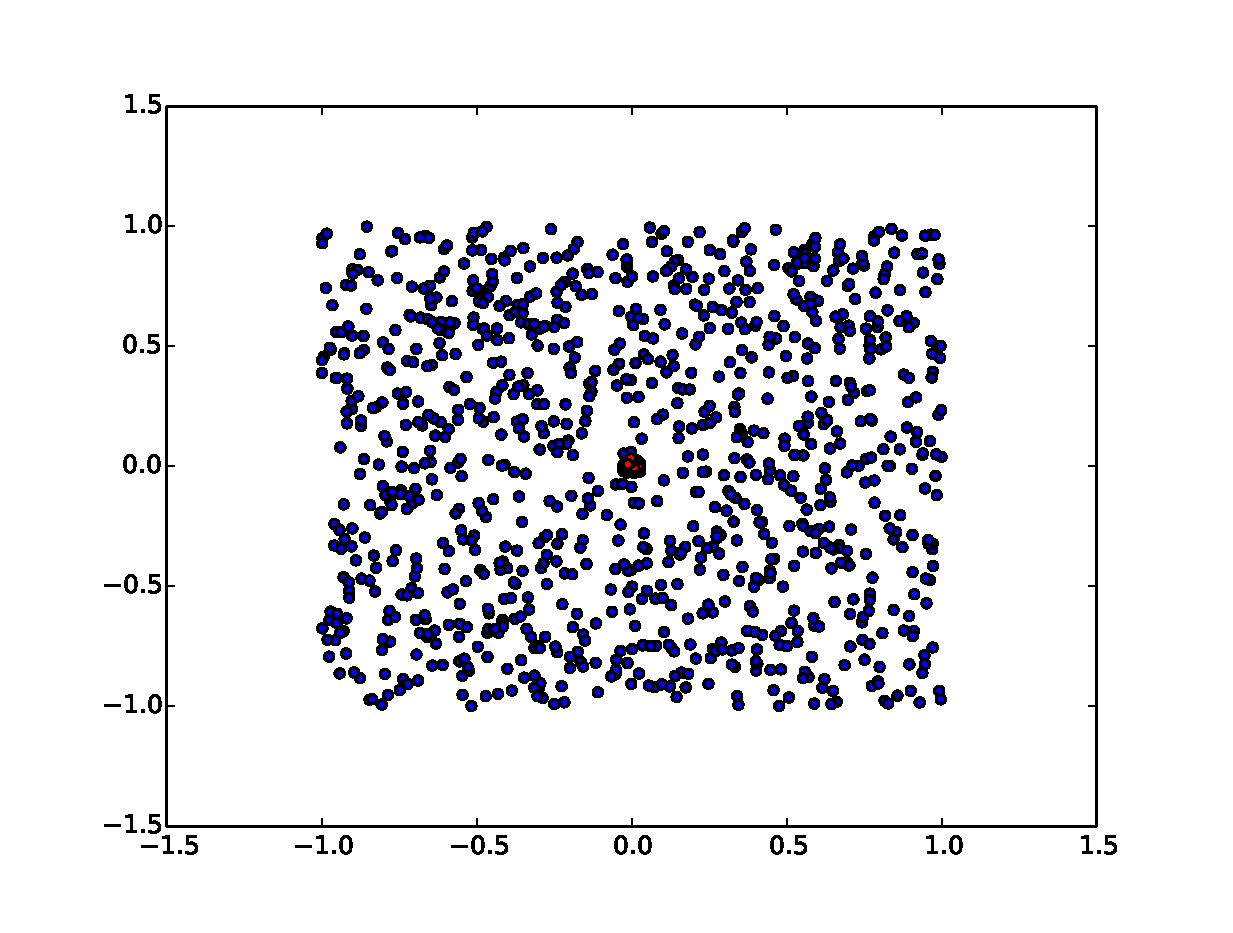
\includegraphics[scale=0.5]{diagrams/pts_plot_sigma0.01.eps}
\caption{Points and sample distributions (2d, sigma = 0.01)}
\label{fig:points_and_sample_2d_0_01}
\end{center}
\end{figure}

\begin{figure}
\begin{center}
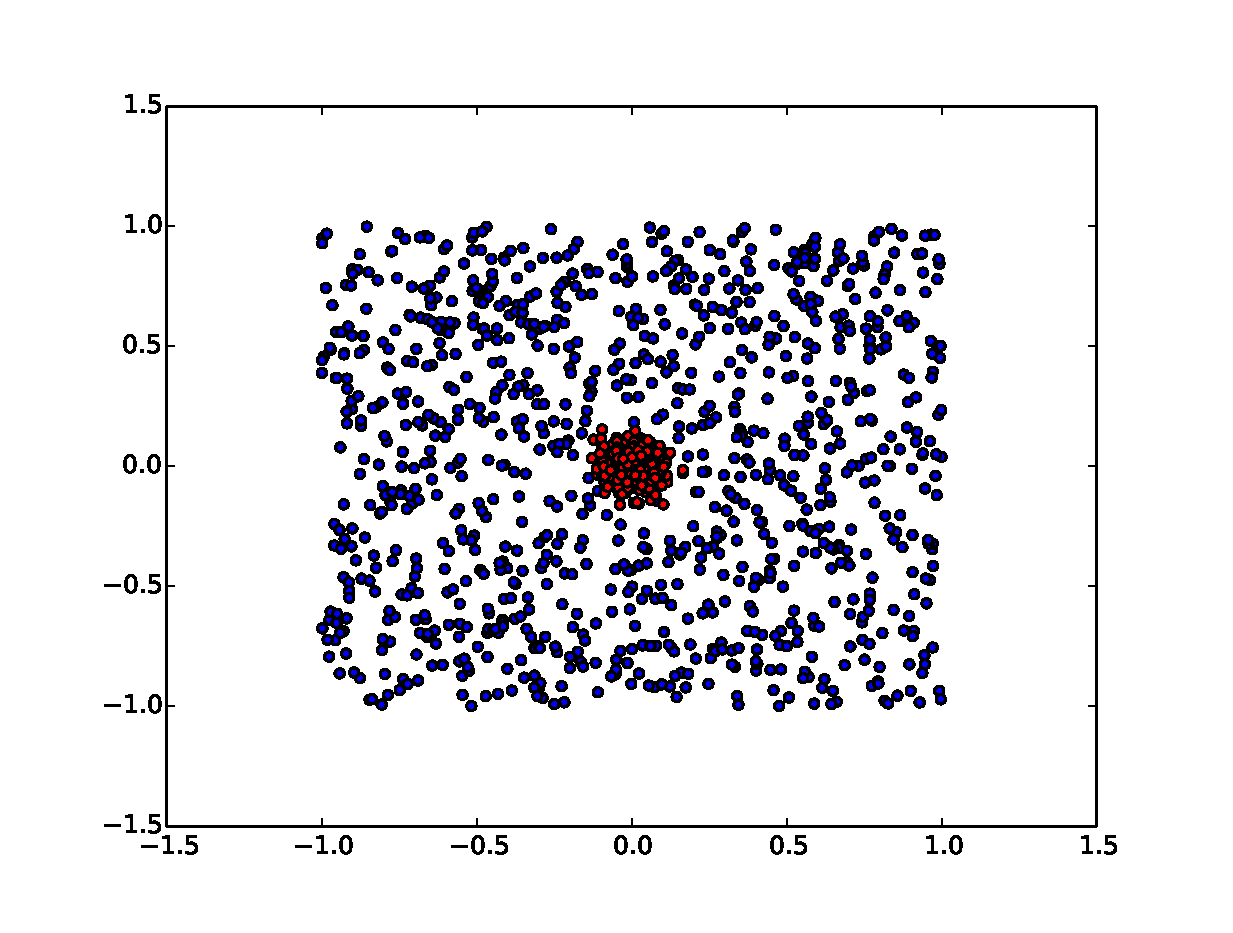
\includegraphics[scale=0.5]{diagrams/pts_plot_sigma0.05.eps}
\caption{Points and sample distributions (2d, sigma = 0.05)}
\label{fig:points_and_sample_2d_0_05}
\end{center}
\end{figure}

\begin{figure}
\begin{center}
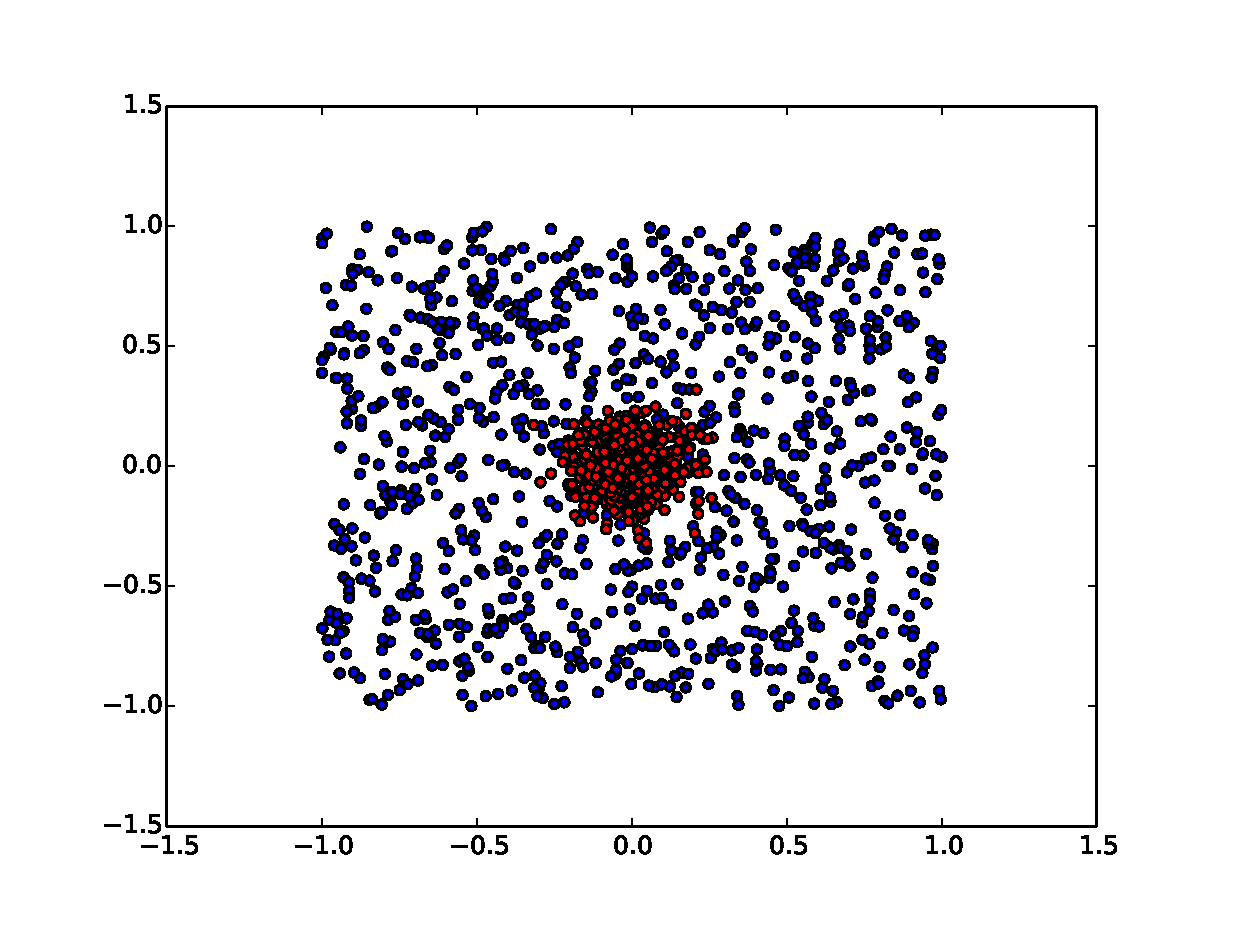
\includegraphics[scale=0.5]{diagrams/pts_plot_sigma0.10.eps}
\caption{Points and sample distributions (2d, sigma = 0.10)}
\label{fig:points_and_sample_2d_0_10}
\end{center}
\end{figure}

\begin{figure}
\begin{center}
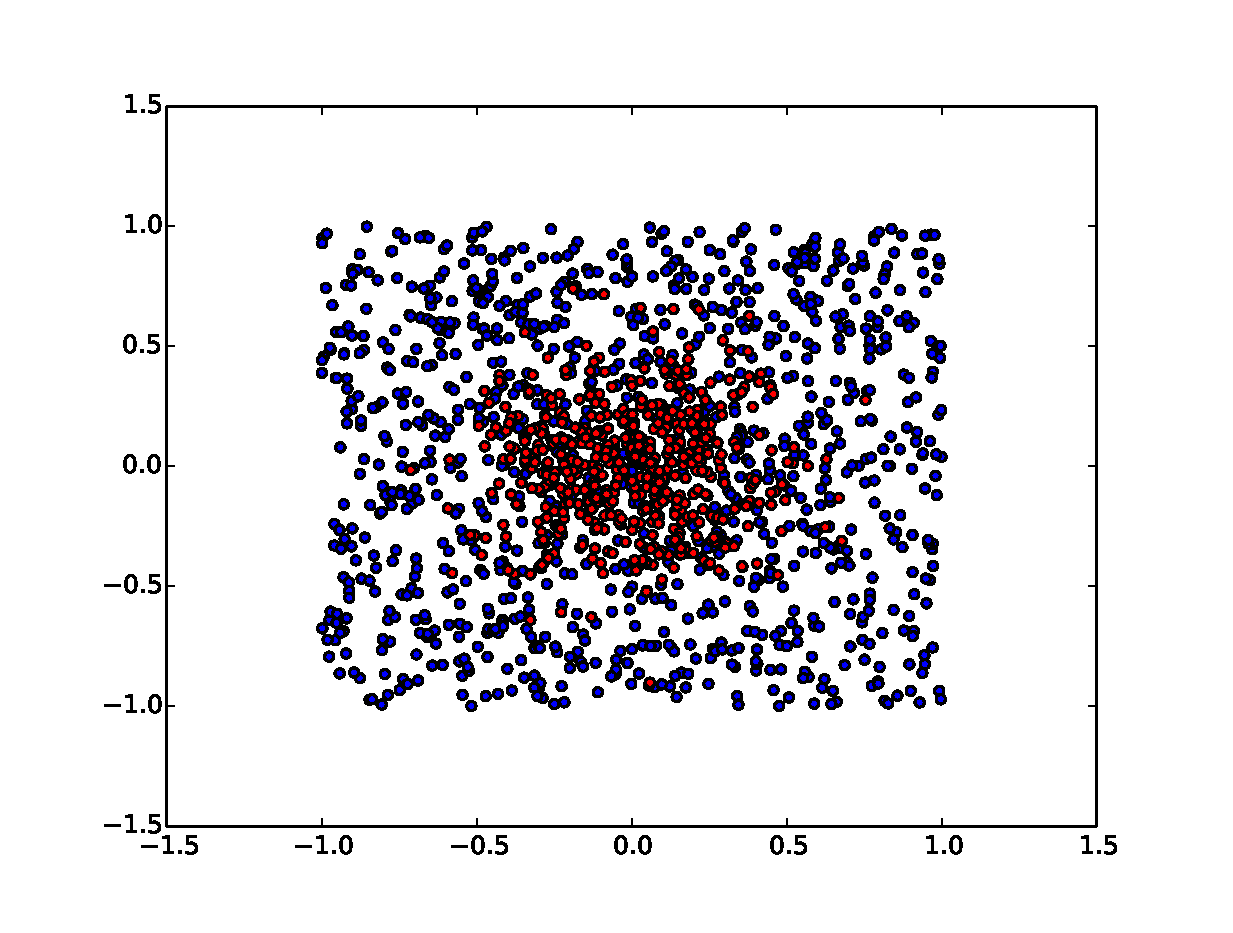
\includegraphics[scale=0.5]{diagrams/pts_plot_sigma0.25.eps}
\caption{Points and sample distributions (2d, sigma = 0.25)}
\label{fig:points_and_sample_2d_0_25}
\end{center}
\end{figure}

\begin{figure}
\begin{center}
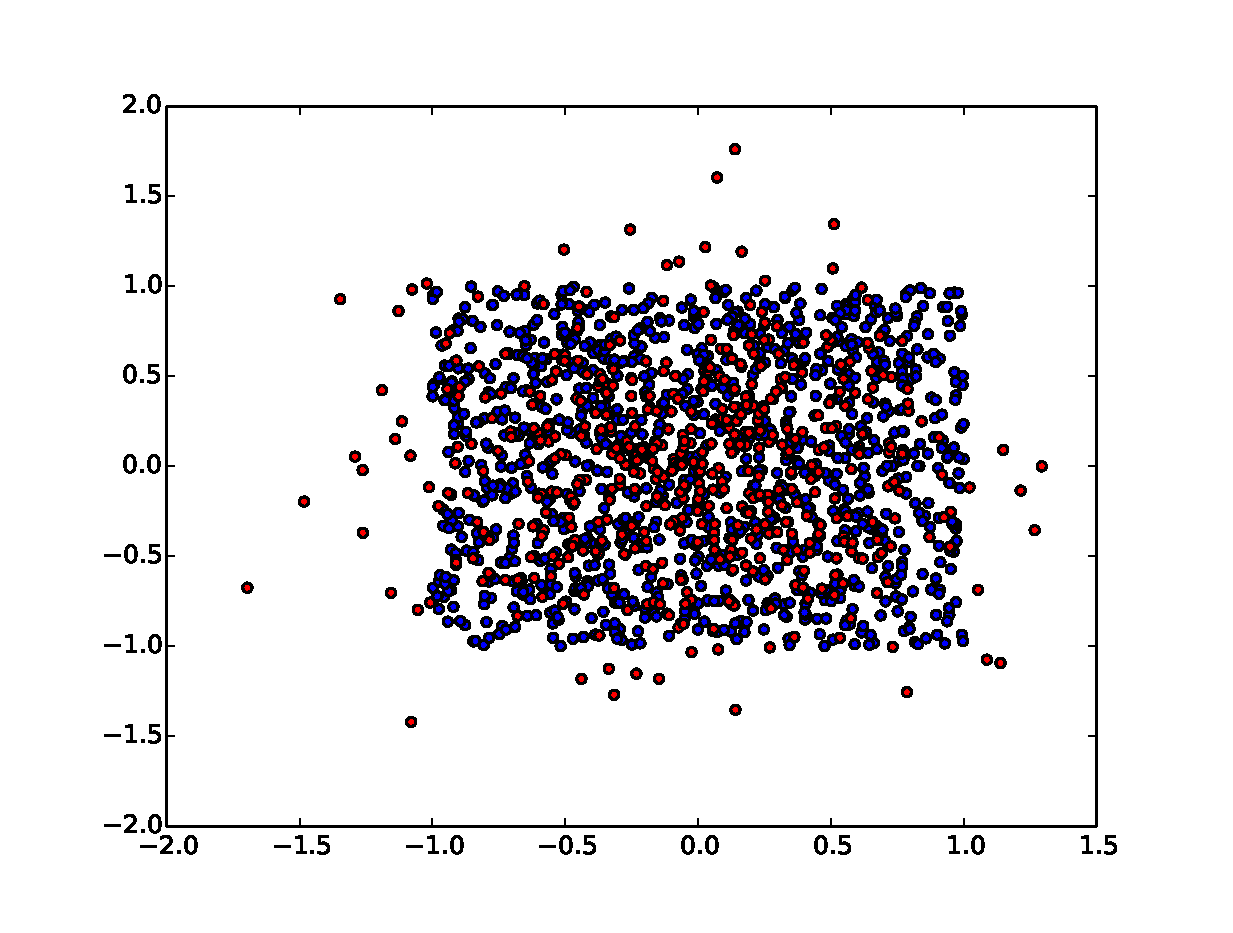
\includegraphics[scale=0.5]{diagrams/pts_plot_sigma0.50.eps}
\caption{Points and sample distributions (2d, sigma = 0.50)}
\label{fig:points_and_sample_2d_0_50}
\end{center}
\end{figure}

For each case the search set consists of 100000 points. In pilot experiments
this size ensured long enough running times to make meaningful comparisons
between experimental cases without requiring an excessive amount of time to
perform all of the experiments. If too few searches are used the runtimes may
end up being within fractions of a second of each other and so much more likely
to be affected by noise.

The experimentation in this thesis is done using synthetic datasets due to the
difficulty in finding existing datasets that include suitable probability
distributions over the searches . This also makes it difficult to demonstrate
that the search distributions chosen reflect ``real-world'' problems.

Although it is possible to take existing datasets and attempt to derive or
create typical search distributions for them, this would essentially still be
using synthetic data because the primary determinant of odds-on tree performance
is the entropy of the sites given a probability distribution over the searches.

\subsection{Sample Set Size}

The sample set is a set of searches used to build the odds-on tree. Each sample
set is created by sampling the same probability distribution used to create the
search set. A different sample set is generated for each run. Example sample
sets are shown in the figures above.

The sample set set size used is $0.5n$, $n$, and $2n$, where $n$ is the
cardinality of the point set. Pilot experimentation showed that these values
provide a reasonable indication of the performance impact of sample set size. 

\subsection{Maximum Build Depth}

The construction of the odds-on tree is controlled by a parameter that 
determines how ``deep'' the recursive build will proceed before terminating.
This parameter will be set be varied between $\log(n)$, $1.5\log(n)$, and
$2\log(n)$ where $n$ is the cardinality of the sample set. Values less than
$\log(n)$ and greater than $2\log(n)$ did not have a substantial impact on
results in the pilot experimentation. 

\subsection{Number of Runs}

Each experimental configuration is repeated ten times with a different sample
set in each case. During pilot experimentation, this was shown to generate
statistically significant differences between configurations for nearly all cases
examined (t-test, $p < 0.0001 $).

\section{Measuring Performance}

\subsection{Benchmark Platform}

The experimentation is done using a virtualized host provided by a third party.
This allows for easy duplication of hardware to run experiments in parallel and
aids in repeatability. Although instance types are eventually retired by
providers, physical hardware is likewise only available for limited period of
time.

The benchmark platform is a Digital Ocean droplet with a 2.4GHz processor, 1 GB
of RAM, and 30 GB SSD secondary storage. During pilot experimentation, the
digital ocean instance was found to be considerably faster and so more
cost-effective than an Amazon Web Services EC2 Medium Compute Optimized
instance, with two 64-bit processors and 1.7GB of RAM. This is likely due to the
Amazon instance type not providing SSD backed storage and so becoming I/O bound 
reading experiment data. 

\subsection{Performance Metric}

The primary performance metric is running time. As mentioned above, the time
required to build the tree and the time required to run the queries are measured
separately, allowing these times to be compared independently of the overall
running time. This is done because the effect of build time can be made
arbitrarily small by increasing the number of queries performed.

A secondary performance metric for the odds-on tree is the cache ``hit rate''.
This is the number of queries answered by the odds-on tree as opposed to the
backup tree. This allows for comparison between the kd-tree based and quadtree
based odds-on tree implementations. 

\section{Results}

This section contains the results and analysis for each experimental
parameter described above and concludes with a comparison of the quadtree and
kd-tree based odds-on tree implementations and their performance relative to
the kd-tree.

\subsection{Dimension}

An increase in dimension caused a corresponding increase in the query time of
the odds-on tree and kd-tree implementations. It also caused the relative
performance of the odds-on tree to become worse. In two or three
dimensions and small search set sigma, the odds-on tree outperforms the kd-tree.
In eight dimensions, even with a favourable search set sigma, the kd-tree
equals or outperforms the odds-on tree in query time. Typical results for a
quadtree based odds-on tree are shown in figure ~\ref{fig:dimension_ctime}. This
decrease in performance is likely caused by the decreased effectiveness of a
fixed sample size as dimensionality increased.

\begin{figure}
\begin{center}
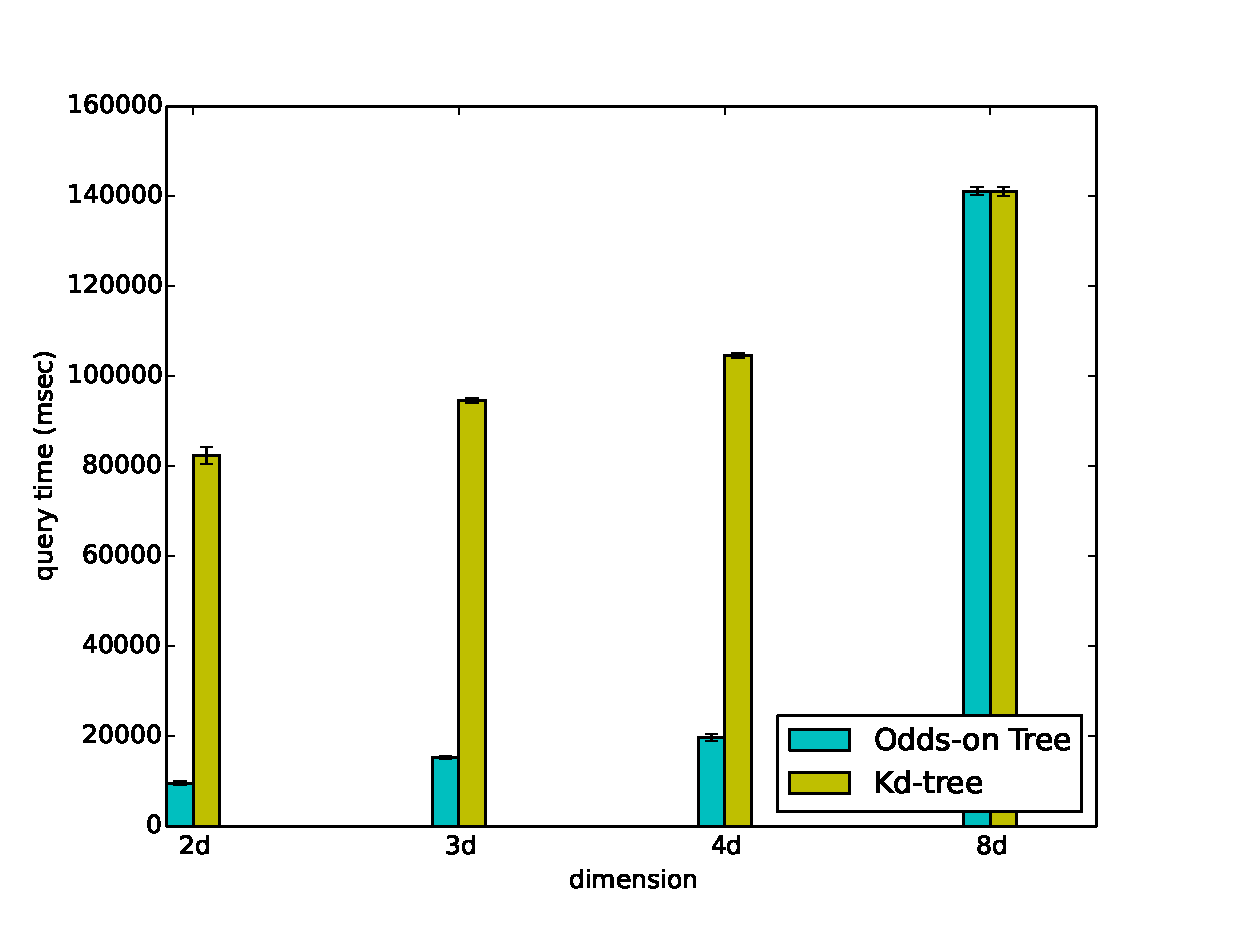
\includegraphics[scale=0.5]{diagrams/dims_pts50000_sample25000_sigma0.01_qtime.eps}
\caption{Query Time (pts = 50000, sample = 25000, sigma = 0.01)}
\label{fig:dimension_ctime}
\end{center}
\end{figure}

Build times likewise became worse for the odds-on tree implementations as
dimensionality increased. The impact on the kd-tree build time was negligible.

\subsection{Point Set Size}

To see the impact of point set size, the build depth and sample sigma are held
constant and the build and construction times are plotted for each point set
size.

For the kd-tree based implementation increasing the point set size increases
build time and query time and query time variance. The kd-tree query time
increases, but the build time is not significantly impacted at the point set
sizes tested, in comparison to the odds-on tree implementation.

\begin{figure}
\begin{center}
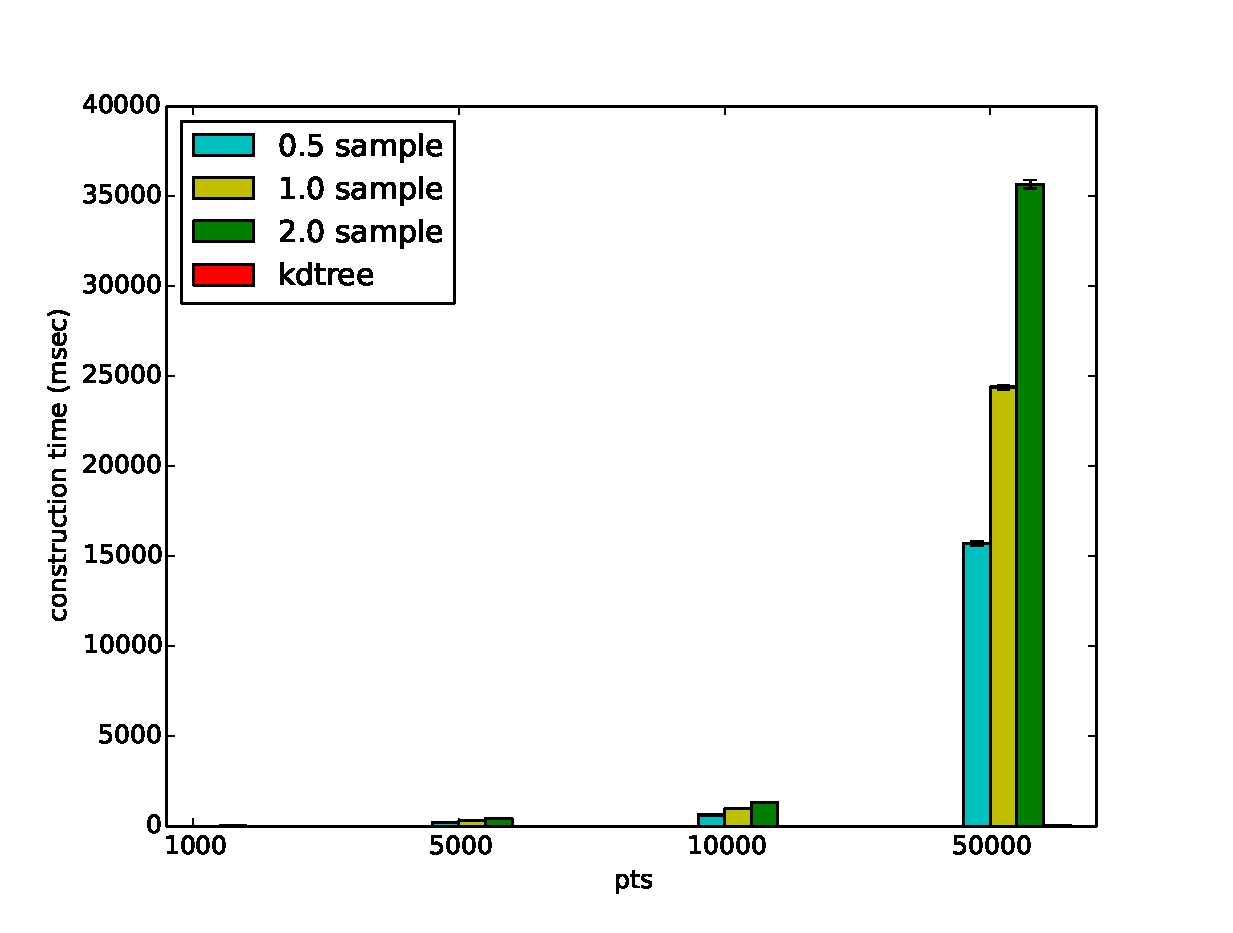
\includegraphics[scale=0.5]{diagrams/2d_group_bypts_sigma0.01_ctime.eps}
\caption{Construction Time (kd-tree, 2d, sigma = 0.01)}
\label{fig:point_set_size_ctime}
\end{center}
\end{figure}

For the most part the relative query performance of the kd-tree based odds-on
tree and kd-tree did not change with increased point set size. If the odds-on tree
outperformed the kd-tree for small point set sizes, it also did so for large
point set sizes. There were a few exceptions at larger search set entropies and
higher dimensions.

\begin{figure}
\begin{center}
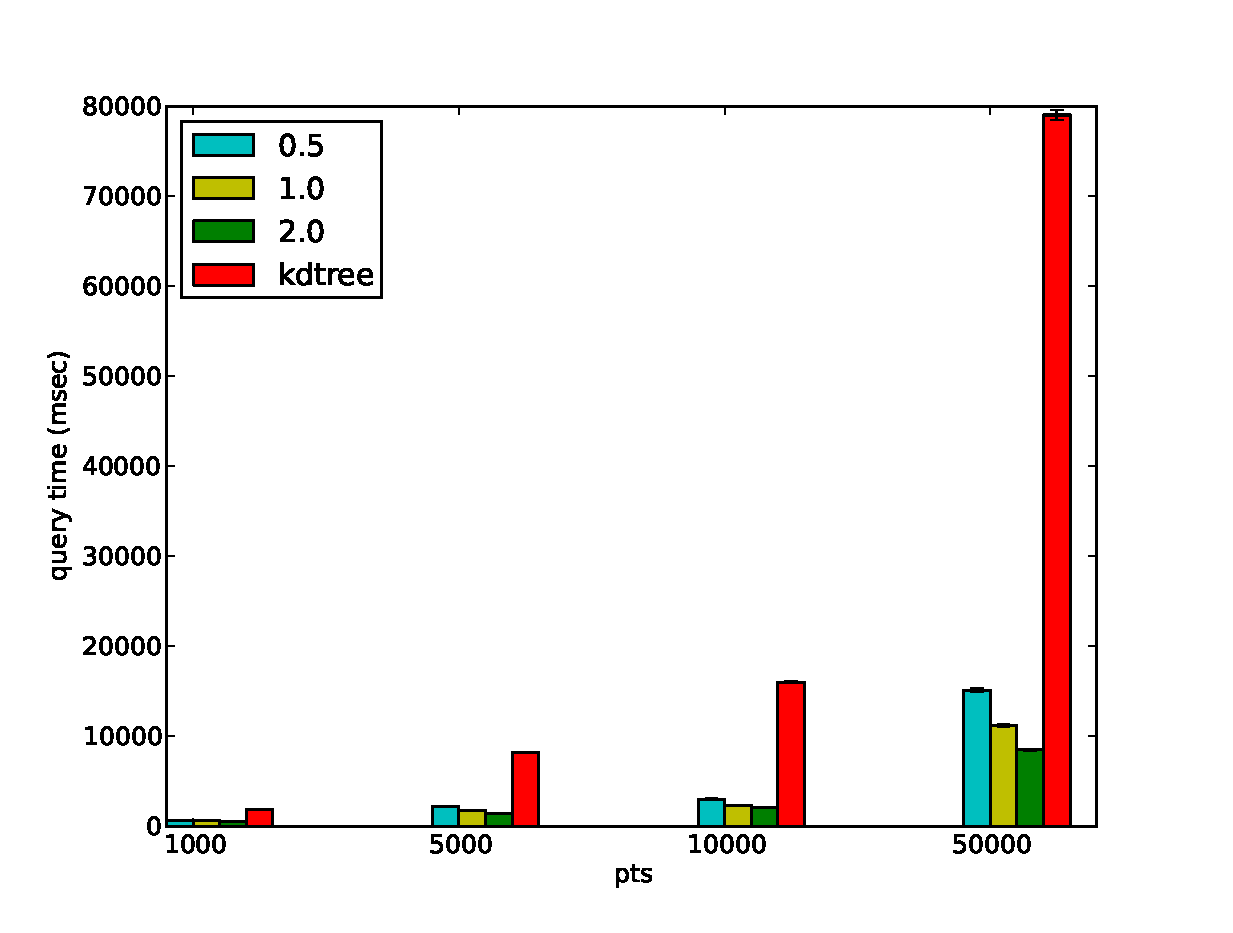
\includegraphics[scale=0.5]{diagrams/2d_group_bypts_sigma0.01_qtime.eps}
\caption{Query Time (kd-tree, 2d, sigma = 0.01)}
\label{fig:point_set_size_qtime}
\end{center}
\end{figure}

The results for the quadtree based odds-on tree follow the same pattern, with
increased point set size increasing the overall running time, but not changing
the relative performance of the odds-on tree and the kd-tree. Typical build
time results are shown in figure ~\ref{fig:point_set_size_ctime_qt} and
construction time results in figure ~\ref{fig:point_set_size_qtime_qt}  

\begin{figure}
\begin{center}
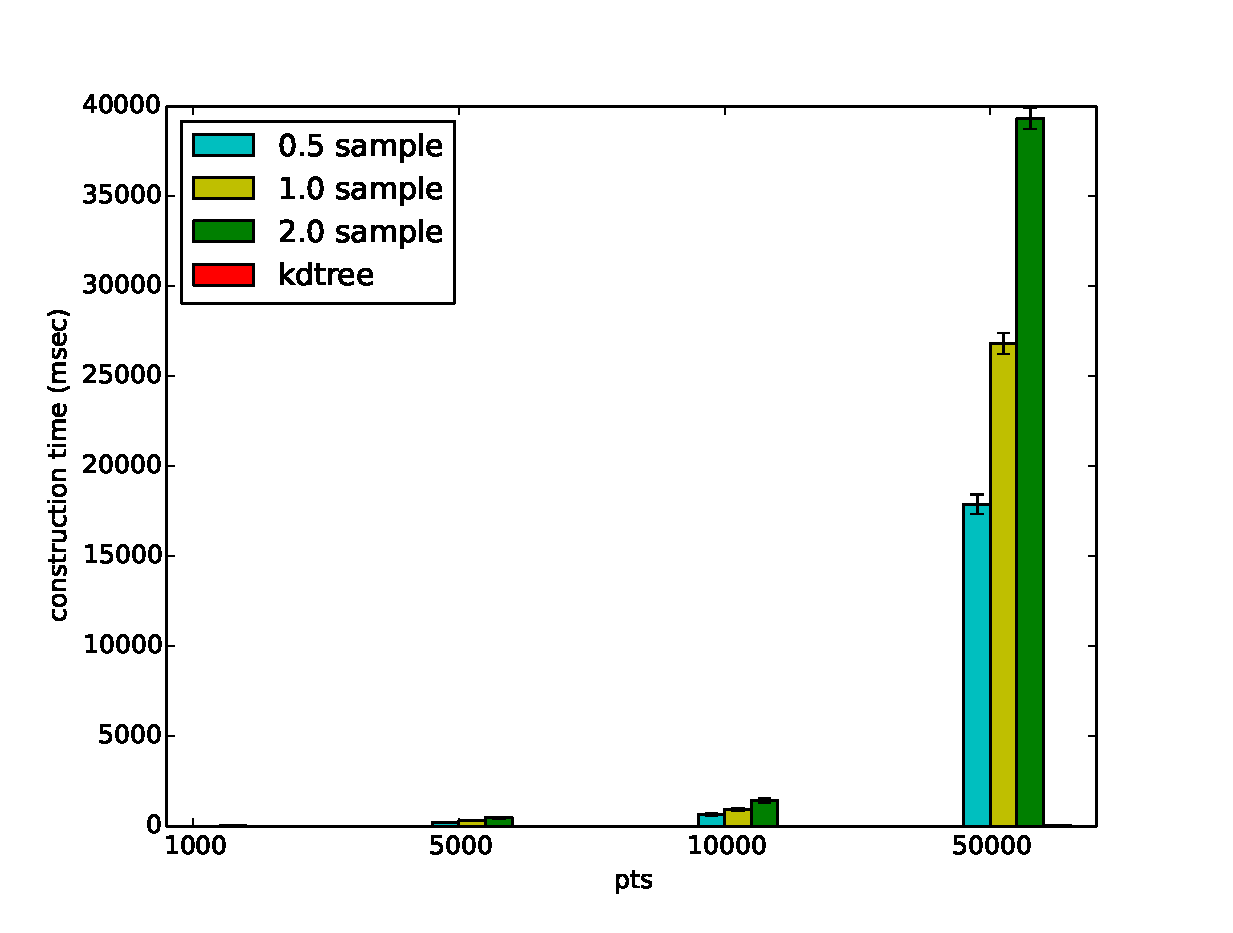
\includegraphics[scale=0.5]{diagrams/2d_group_bypts_sigma0.01_ctime_qt.eps}
\caption{Construction Time (quadtree, 2d, sigma = 0.01)}
\label{fig:point_set_size_ctime_qt}
\end{center}
\end{figure}

\begin{figure}
\begin{center}
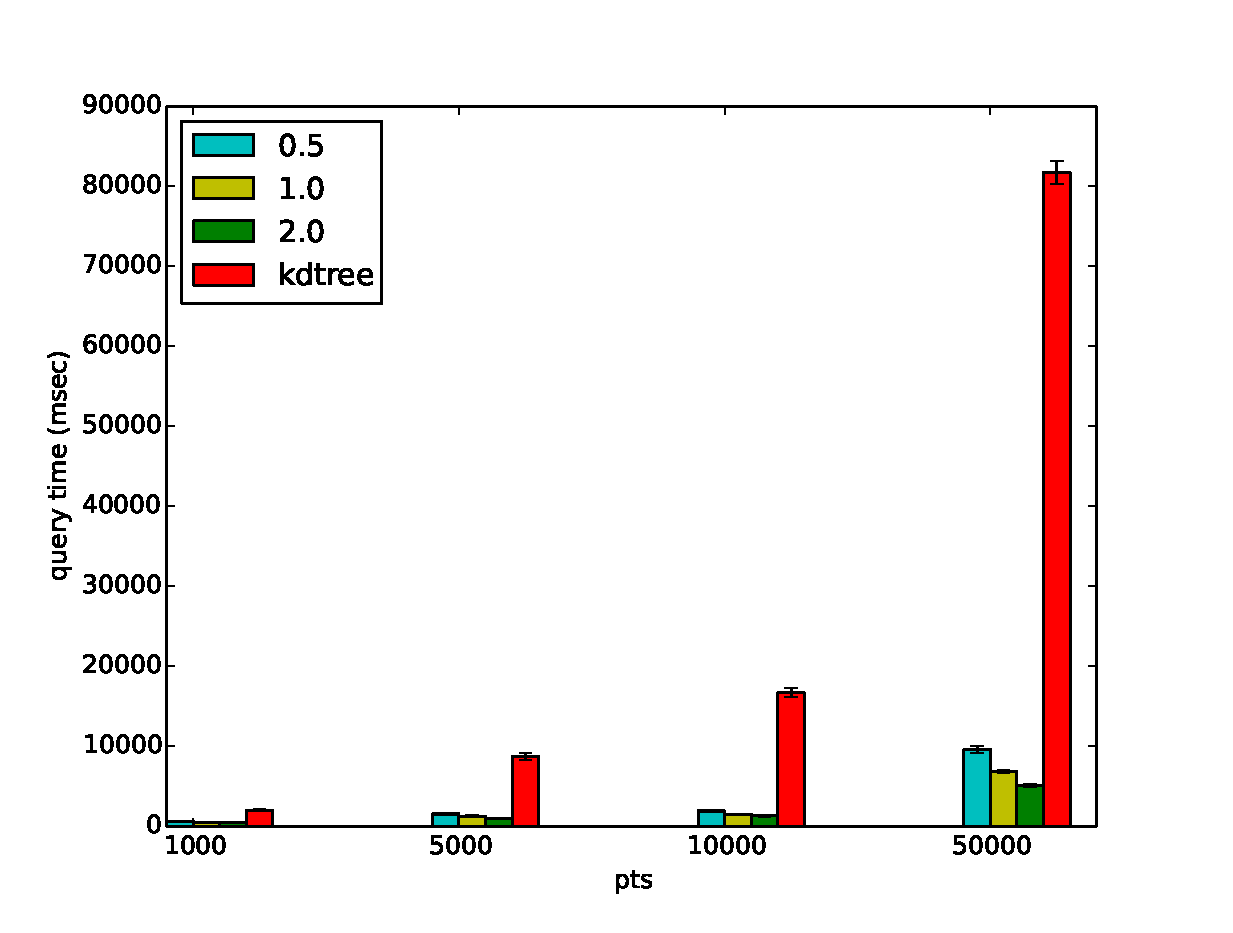
\includegraphics[scale=0.5]{diagrams/2d_group_bypts_sigma0.01_qtime_qt.eps}
\caption{Query Time (quadtree, 2d, sigma = 0.01)}
\label{fig:point_set_size_qtime_qt}
\end{center}
\end{figure}

\subsection{Search Set Entropy}

Increasing sigma value causes the performance of the odds-on tree to
At small sigma values, the odds-on tree performs significantly better than
the kd-tree. As sigma increases, the odds-on tree begins to perform worse
until its performance is more or less equivalent, indicating that almost
all queries are being handled by the backup kd-tree rather than the odds-on
tree itself.

As sigma increases, the performance of the kd-tree itself also improves.
This is due to the kd-tree doing less backtracking to determine if the
candidate nearest-neighbour is in fact the actual nearest-neighbour at
larger sigma values. For sigma = 0.25, the kd-tree does 17 percent less
backtracking, and for sigma = 0.5 the kd-tree does 35 percent less
backtracking. This is in turn a side effect of the searches being centered
around the origin. As sigma increases, the searches are more likely to
fall on the periphery of the kd-tree, meaning less nodes inside the
kd-tree need to be visited while backtracking to find the nearest
neighbour. Figure ~\ref{fig:sigma_qtime} shows query time results for a 2d
kd-tree based odds-on tree..

\begin{figure}
\begin{center}
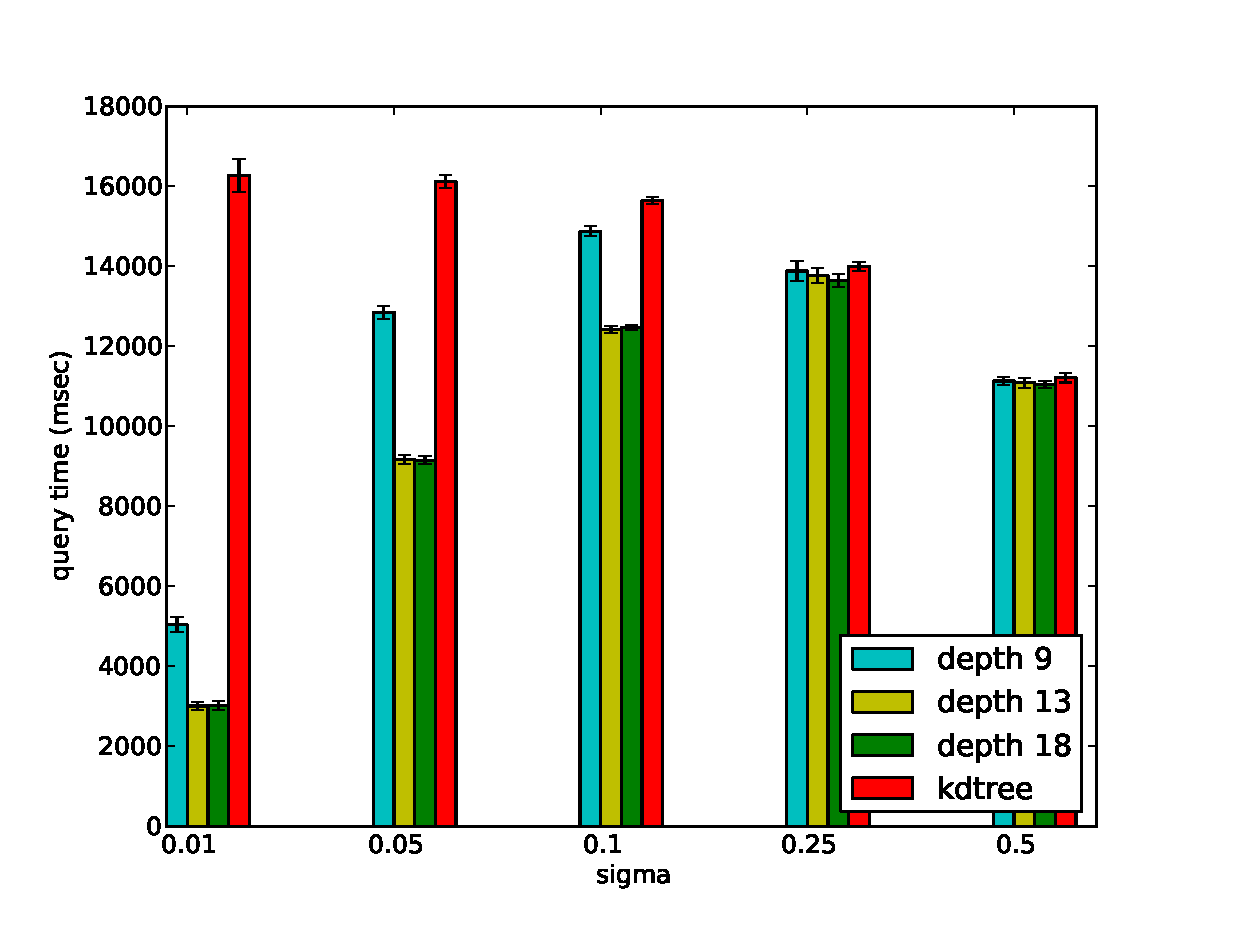
\includegraphics[scale=0.5]{diagrams/2d_pts10000_sample5000_qtime.eps}
\caption{Query Time (kd-tree, 2d, pts=10000, sample=5000)}
\label{fig:sigma_qtime}
\end{center}
\end{figure}

The construction time for the kd-tree based odds-on tree implementation worsens
as sigma increases until it reaches a maximum at a sigma of 0.1. At this point,
the construction time begins to decrease. This decrease matches the decrease
in query time for the kd-tree at those sigma values. Since constructing the
odds-on tree requires a large number of kd-tree based nearest neighbour
searches, the improved kd-tree performance also benefits the construction time
for the odds-on tree. Figure ~\ref{fig:sigma_ctime} shows construction time
results for a 2d kd-tree based odds-on tree..

\begin{figure}
\begin{center}
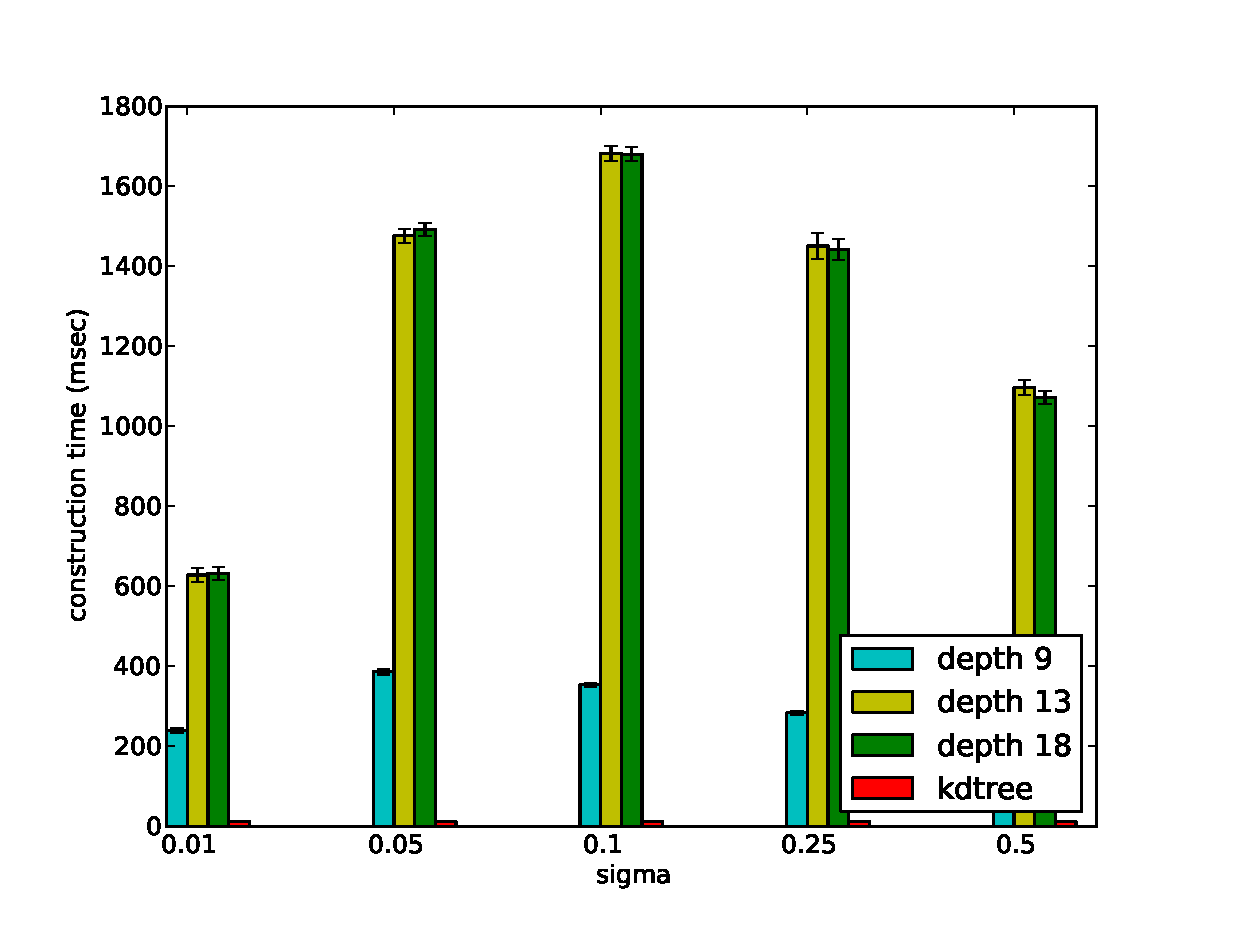
\includegraphics[scale=0.5]{diagrams/2d_pts10000_sample5000_ctime.eps}
\caption{Construction Time (kd-tree, 2d, pts=10000, sample=5000)}
\label{fig:sigma_ctime}
\end{center}
\end{figure}

The observed decrease in performance with increasing sigma values is due to
a larger odds-on tree being built. The number of terminal nodes remains
relatively small while the overall size of the odds-on tree and the number of
nearest neighbour queries required increases substantially. Typical results are
shown in figure ~\ref{fig:node_counts}.

\begin{figure}
\begin{center}
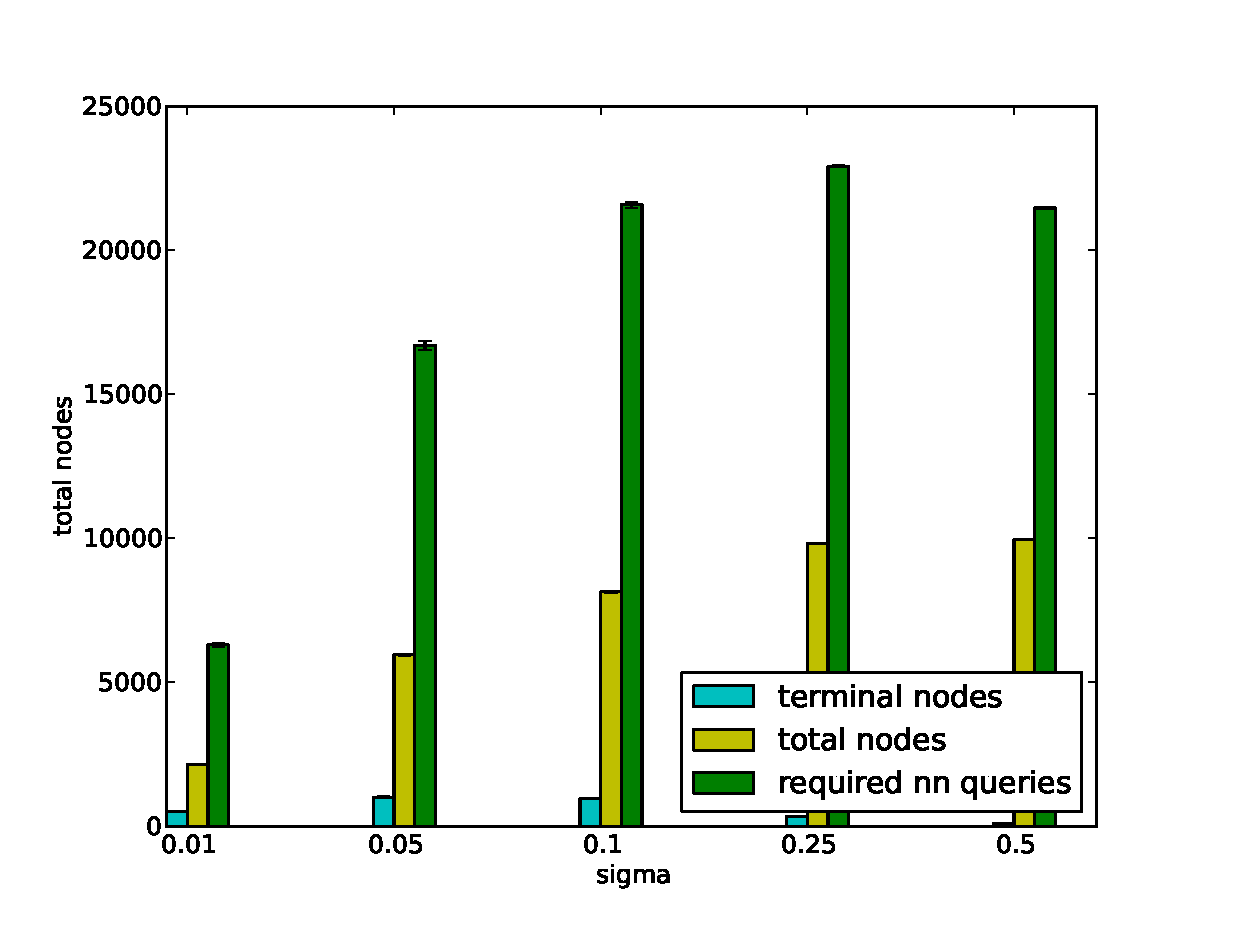
\includegraphics[scale=0.5]{diagrams/2d_pts10000_sample10000_builddata.eps}
\caption{Node Counts (kd-tree, 2d, pts=10000, sample=10000, build depth=13)}
\label{fig:node_counts}
\end{center}
\end{figure}

\subsection{Sample Set Size}

The sample set size has a direct impact on build and query times. Increasing
the sample set size requires more time to build due to additional nearest
neighbour queries during the cache construction, but usually results in a
better cache, causing the a corresponding decrease in query time.  An example
of typical build time results are shown in figure
~\ref{fig:sample_set_size_qtime} and query time results are in figure
~\ref{fig:sample_set_size_ctime}.

\begin{figure}
\begin{center}
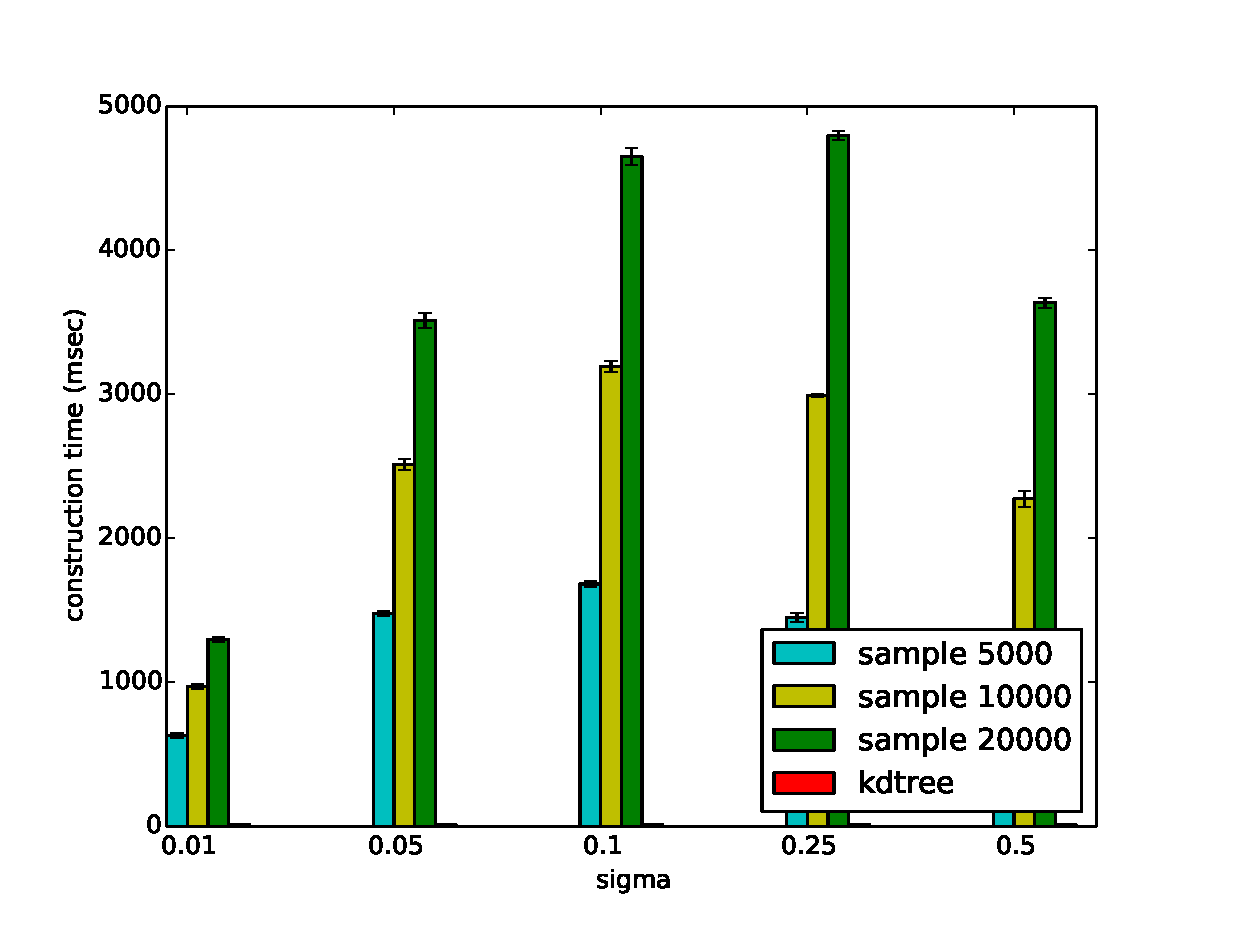
\includegraphics[scale=0.5]{diagrams/kt_2d_pts10000_groupbysample_ctime.eps}
\caption{Construction Time(kd-tree, 2d, pts=10000)}
\label{fig:sample_set_size_ctime}
\end{center}
\end{figure}

\begin{figure}
\begin{center}
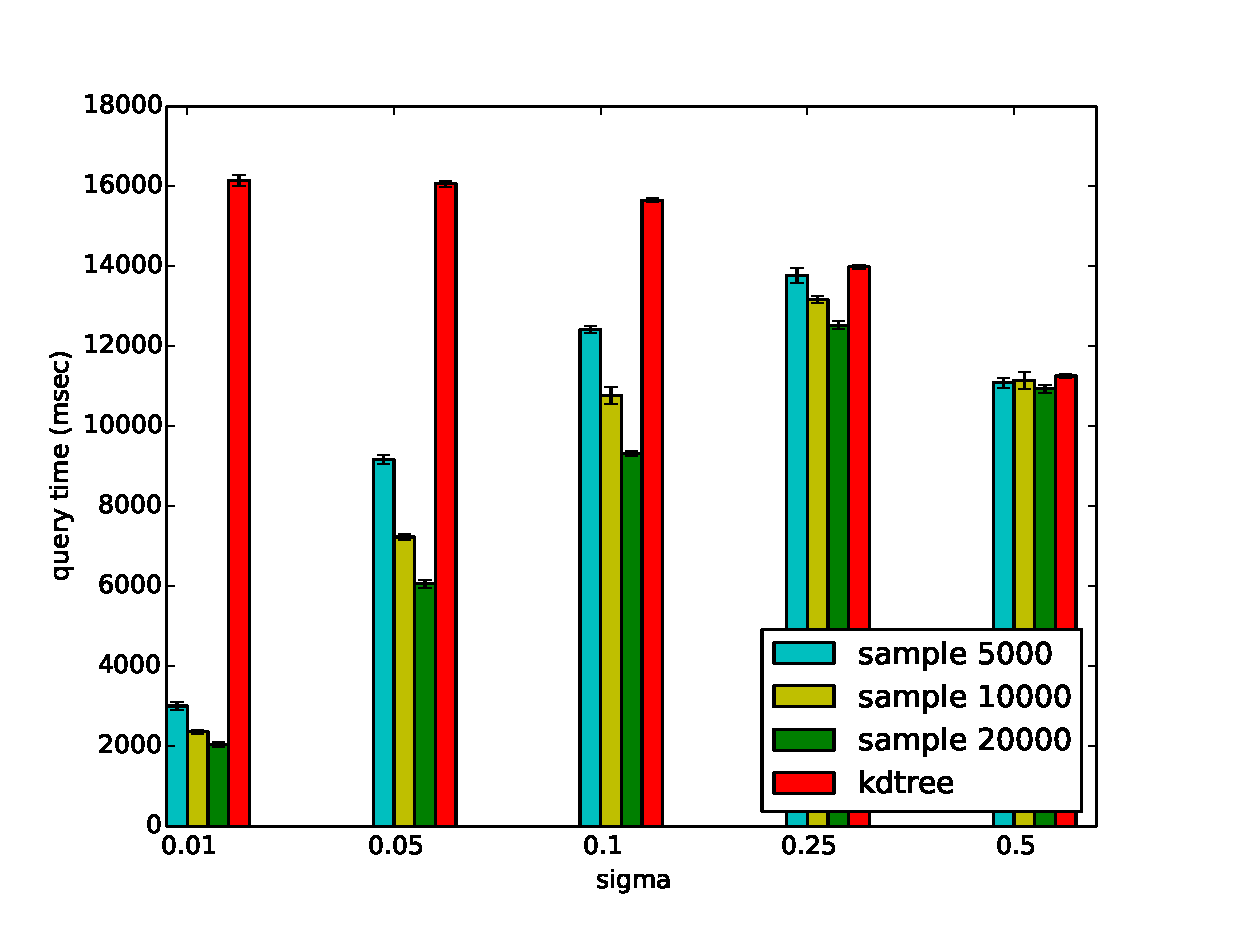
\includegraphics[scale=0.5]{diagrams/kt_2d_pts10000_groupbysample_qtime.eps}
\caption{Query Time(kd-tree, 2d, pts=10000)}
\label{fig:sample_set_size_qtime}
\end{center}
\end{figure}

Because changing sample set size is a trade off between build time and query
time, it makes sense to present results for total time. A typical result for
overall running time is shown in figure ~\ref{fig:sample_set_size_total}. For
lower sigma values the higher quality cache that results from a larger sample
set size results in a lower overall running time. As sigma increases, this
benefit decreases until performance becomes roughly equivalent for all sample
set sizes, and before finally becoming worse for larger sample set size, at
which point the kd-tree outperforms the odds-on tree.

\begin{figure}
\begin{center}
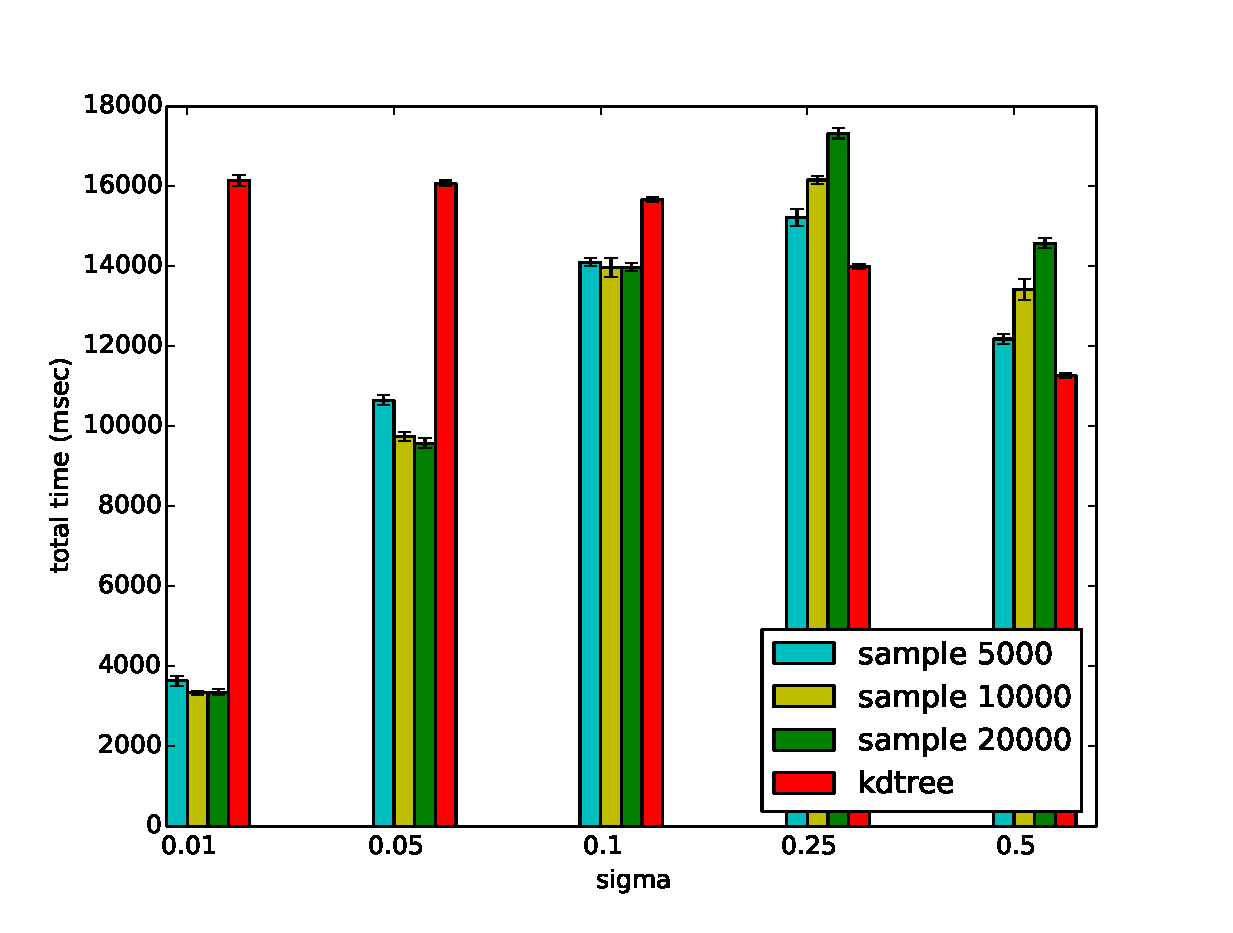
\includegraphics[scale=0.5]{diagrams/kt_2d_pts10000_groupbysample_total.eps}
\caption{Total Time(kd-tree, 2d, pts=10000)}
\label{fig:sample_set_size_total}
\end{center}
\end{figure}

Increasing the sample set size increases both the number of terminal nodes and
the total number of nodes in the odds-on tree as can bee seen in figure
~\ref{fig:sample_set_size_nodecounts}. The overall ratio of terminal nodes to
total nodes is highly dependent on the search set entropy. At low entropy,
increasing the sample set size increases the number of terminal nodes while
maintaining a small overall odds-on tree size. This means that the odds-on
tree is quick to search, and searching it is likely to result in finding a
terminal node. This is not the case at higher search set entropy values.

\begin{figure}
\begin{center}
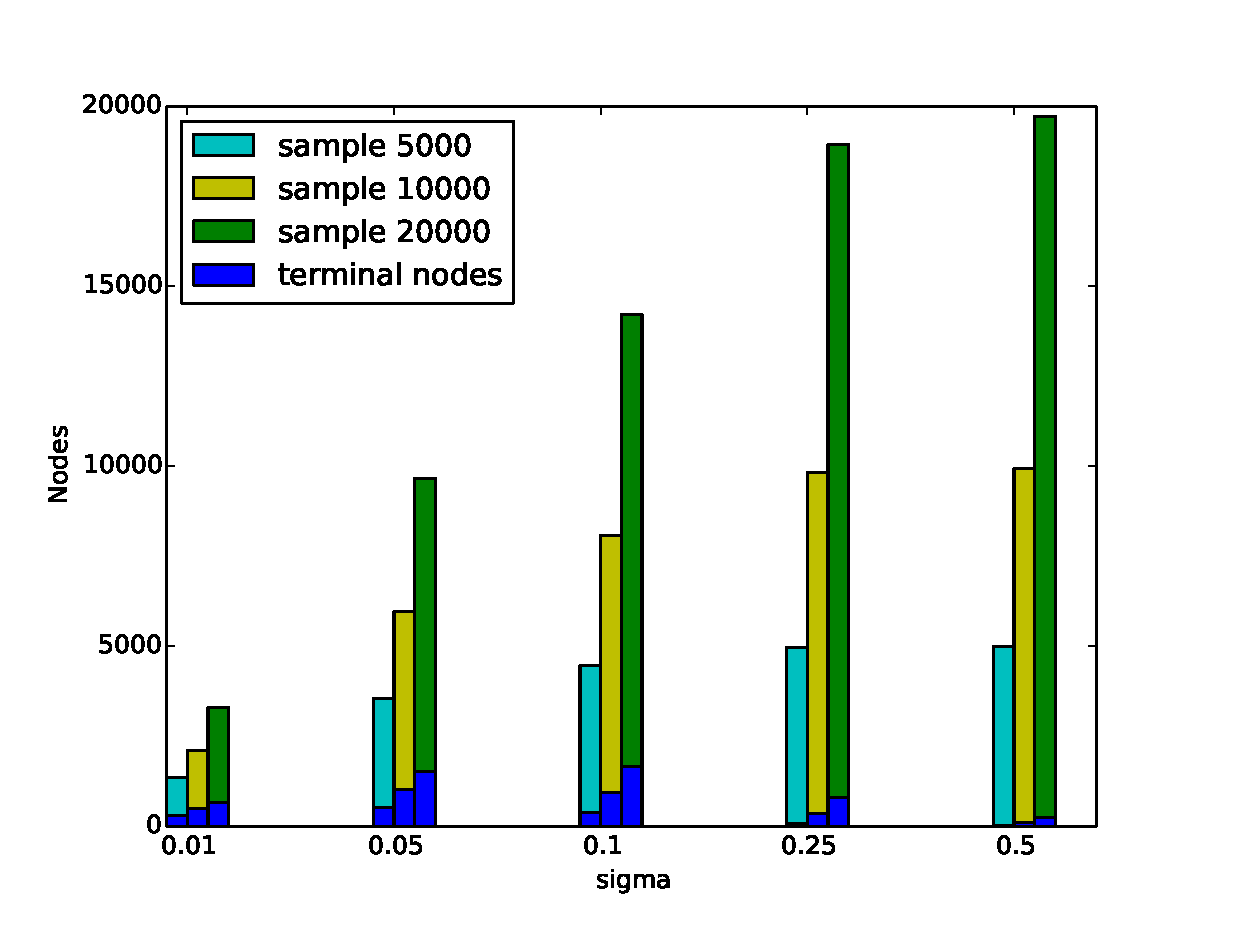
\includegraphics[scale=0.5]{diagrams/kt_2d_nodecounts_pts10000_groupbysample.eps}
\caption{Node Counts (kd-tree, 2d, pts=10000)}
\label{fig:sample_set_size_nodecounts}
\end{center}
\end{figure}

\subsection{Maximum Build Depth}

The maximum build depth parameter limits how deep the odds-on tree will be
built, which affects both construction time and query time. The smallest build
depth value ($\log(n)$, where $n$ is the point set size) investigated typically
results in faster construction time but slower query times and slower overall
performance.

The results for the other two build depth values ($1.5\log(n)$, $2\log(n)$)
are typically very close together.  Example results for build time are shown in
figure ~\ref{fig:max_build_depth_ctime} and for query time are shown in figure
~\ref{fig:max_build_depth_qtime}.

\begin{figure}
\begin{center}
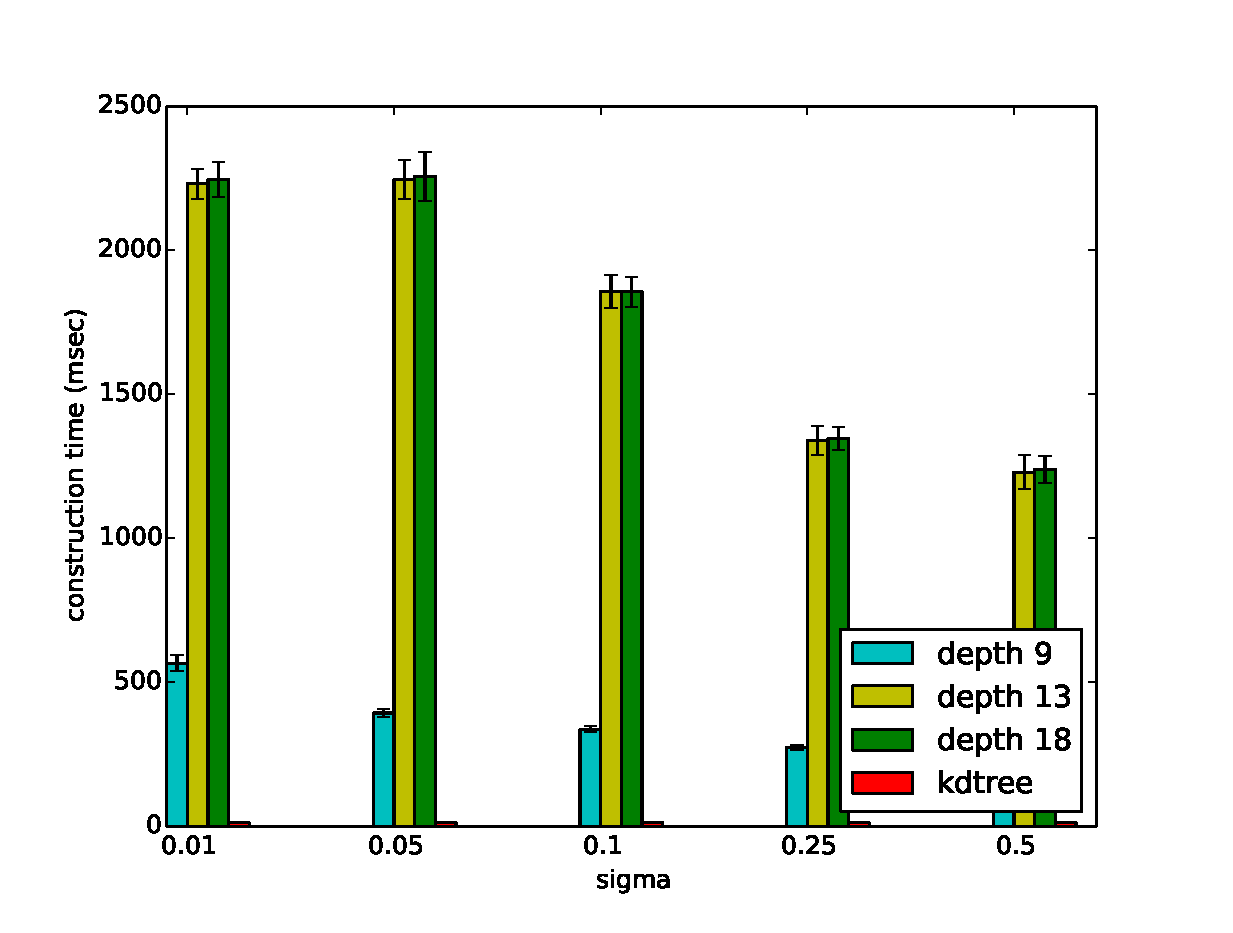
\includegraphics[scale=0.5]{diagrams/kt_3d_pts10000_sample5000_ctime.eps}
\caption{Construction Time(kd-tree, 3d, pts=10000, sample=5000)}
\label{fig:max_build_depth_ctime}
\end{center}
\end{figure}

\begin{figure}
\begin{center}
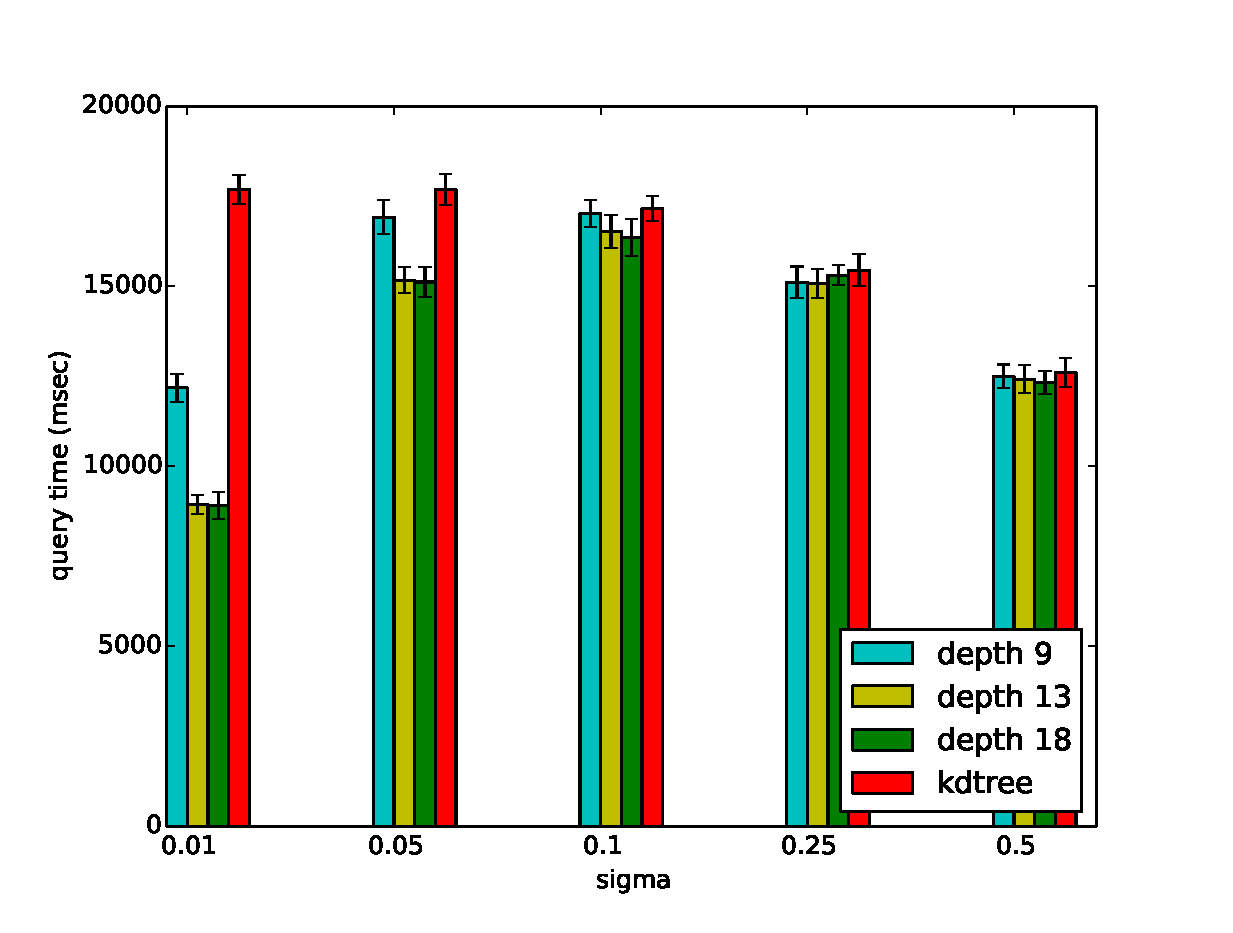
\includegraphics[scale=0.5]{diagrams/kt_3d_pts10000_sample5000_qtime.eps}
\caption{Query Time(kd-tree, 3d, pts=10000, sample=5000)}
\label{fig:max_build_depth_qtime}
\end{center}
\end{figure}

As with sample set size, build depth is a trade off between build time and query
time. A typical result for overall running time is shown in figure
~\ref{fig:max_build_depth_total}. In this case the trees with greater depth are
faster for the sigma = 0.01 condition, but the additional build time ends up
making them slower overall for greater sigma values. 

\begin{figure}
\begin{center}
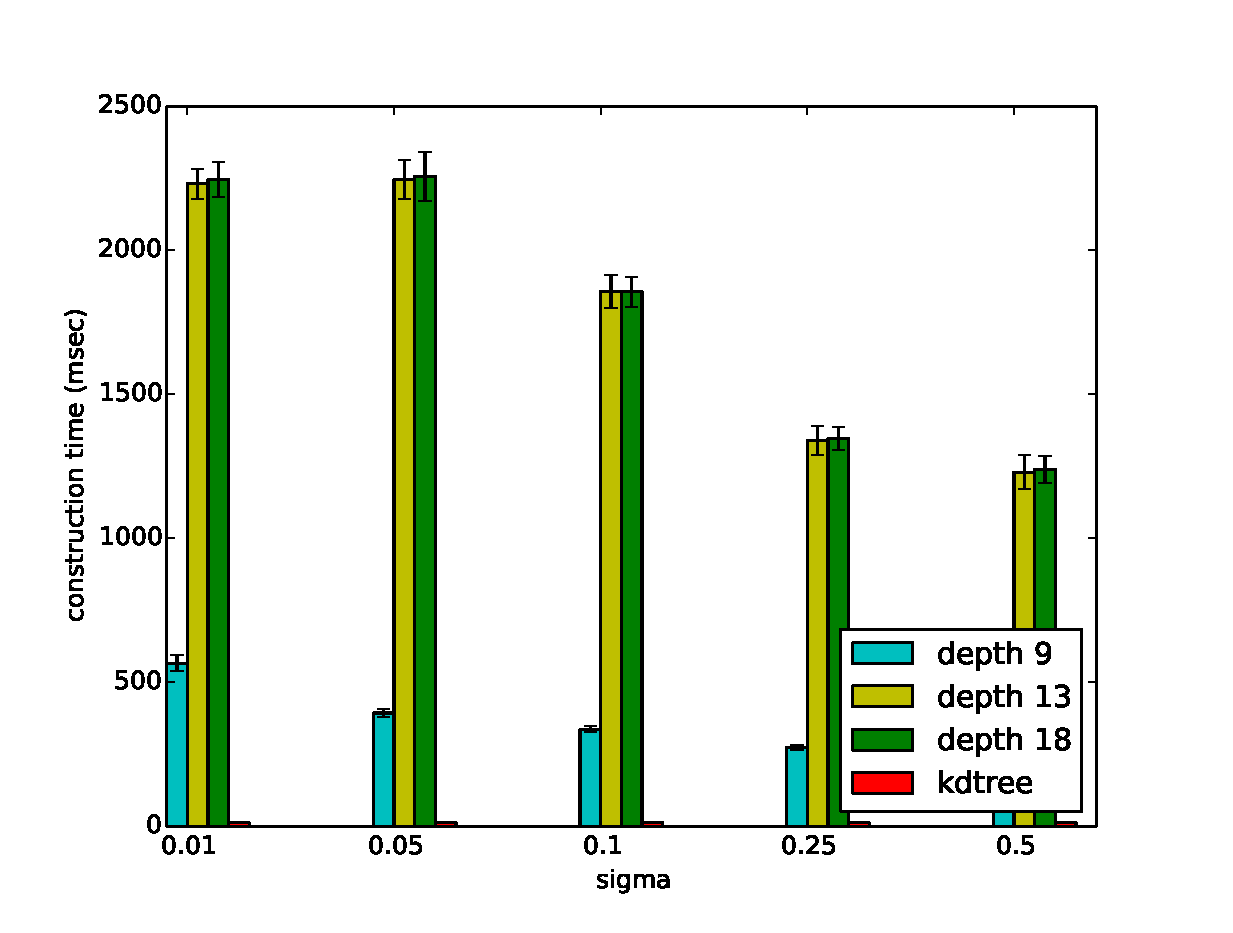
\includegraphics[scale=0.5]{diagrams/kt_3d_pts10000_sample5000_ctime.eps}
\caption{Total Time(kd-tree, 3d, pts=10000, sample=5000)}
\label{fig:max_build_depth_total}
\end{center}
\end{figure}

In comparison to the sample set size, the maximum build depth parameter has
a much less predictable effect on the performance of the odds-on tree. Based
upon the results here, it seems best to set it at a moderate value, say between
$1.25\log(n)$ and $1.5\log(n)$ and use sample set size to make trade offs
between build time and construction time of the odds-on tree.

For the quadtree based odds-on tree there is a lot of variance in the running
time and the build depth parameter does not seem to have a significant impact
on either build time or construction time. As with the kd-tree based
implementation, it seems best to set it at moderate values and use the sample
set size, which has more predictable impact on performance.

\begin{figure}
\begin{center}
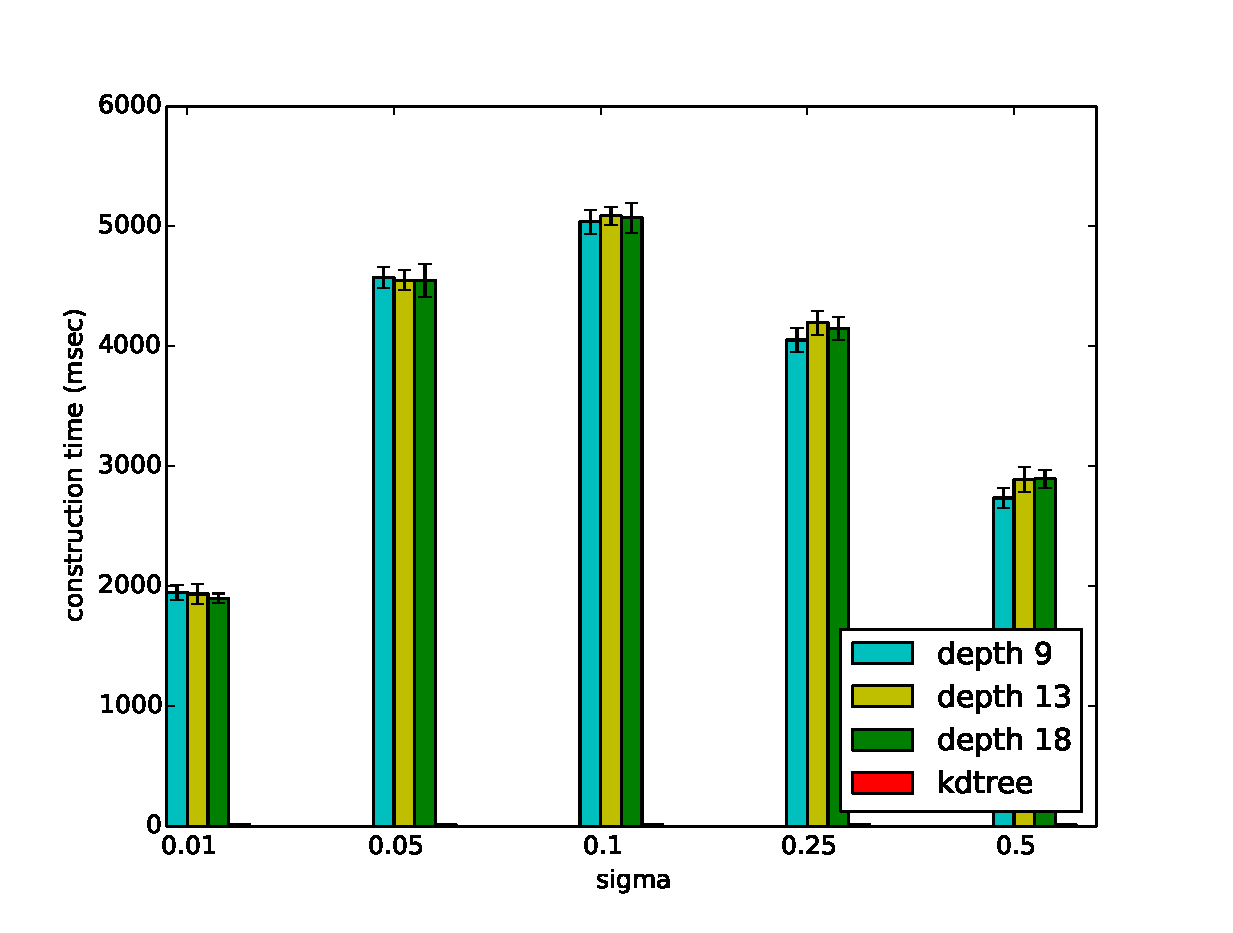
\includegraphics[scale=0.5]{diagrams/qt_3d_pts10000_sample5000_ctime.eps}
\caption{Construction Time(quadtree, 3d, pts=10000, sample=5000)}
\label{fig:max_build_depth_ctime_qt}
\end{center}
\end{figure}

\begin{figure}
\begin{center}
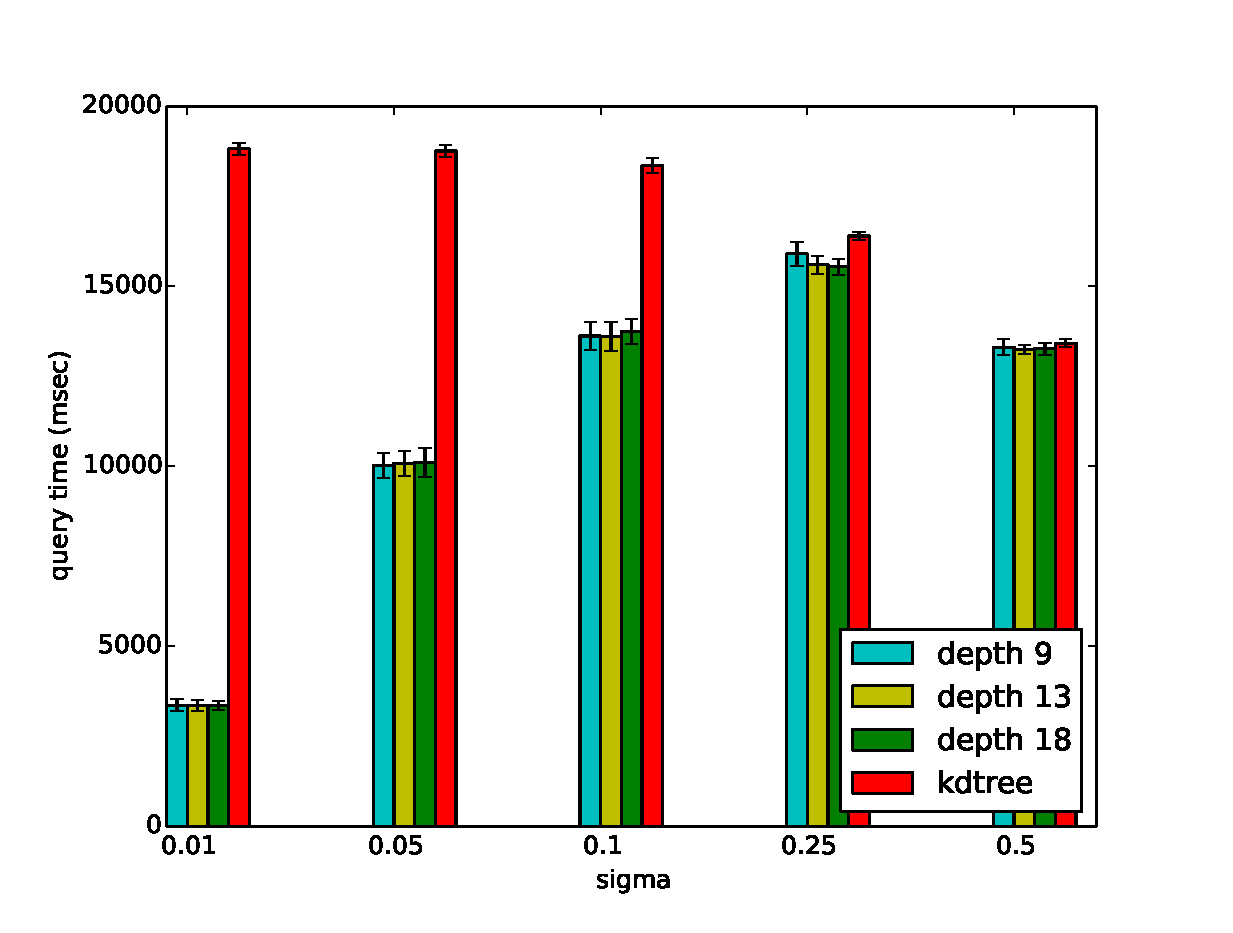
\includegraphics[scale=0.5]{diagrams/qt_3d_pts10000_sample5000_qtime.eps}
\caption{Query Time(quadtree, 3d, pts=10000, sample=5000)}
\label{fig:max_build_depth_qtime_qt}
\end{center}
\end{figure}

\subsection{Quadtree vs. Kd-Tree Based Implementation}

Pilot experimentation did not show either the kd-tree or quadtree based
implementation to be consistently better than the other. In worst case analysis,
kd-trees are expected to exhibit better performance than compressed quadtrees
for nearest neighbour search, but this is not necessarily the case for the
experimental conditions investigated in this thesis.

The quadtree build times are generally worse than the kd-tree based build times.
A kd-tree can be built efficiently by sorting in place, but constructing a
compressed quadtree using a recursive top-down procedure requires allocating
space for new nodes, copying points into them, and then potentially pruning them
after the face. It is possible to build compressed quadtrees based upon sorting
points (see the section on z-order above) but pilot experiments found that
constructing quadtrees this way is faster, but resulted in lower quality caches
so that overall running time was slower.

\begin{figure}
\begin{center}
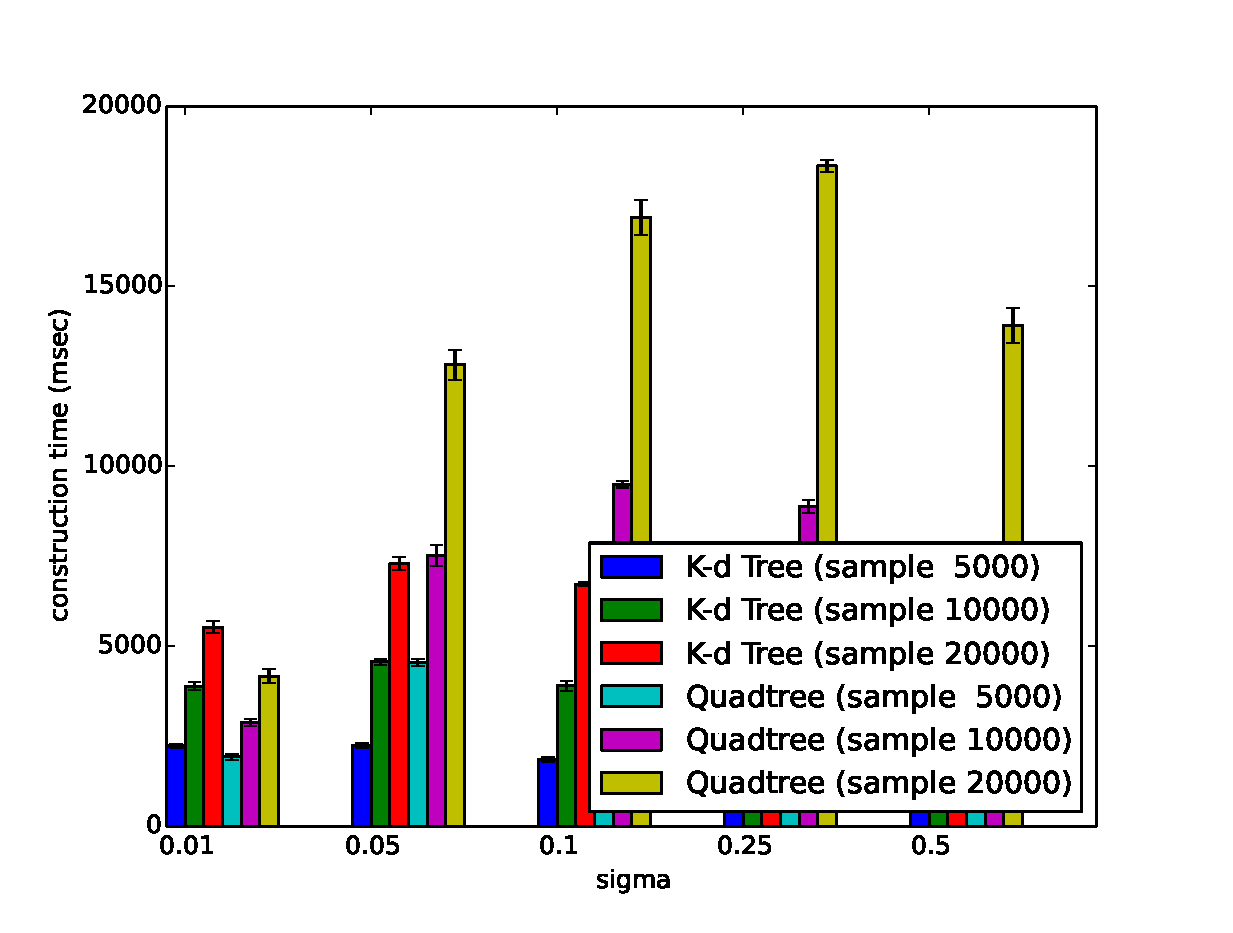
\includegraphics[scale=0.5]{diagrams/3d_qt_kt_pts10000_ctime.eps}
\caption{Build Time(3d, pts=10000)}
\label{fig:3d_kd_qt_ctime}
\end{center}
\end{figure}

For query time it is found that for conditions under which the odds-on tree
performs well (sigma \(\le 0.1\)), the quadtree based implementation will
outperform the kd-tree based implementation.

\begin{figure}
\begin{center}
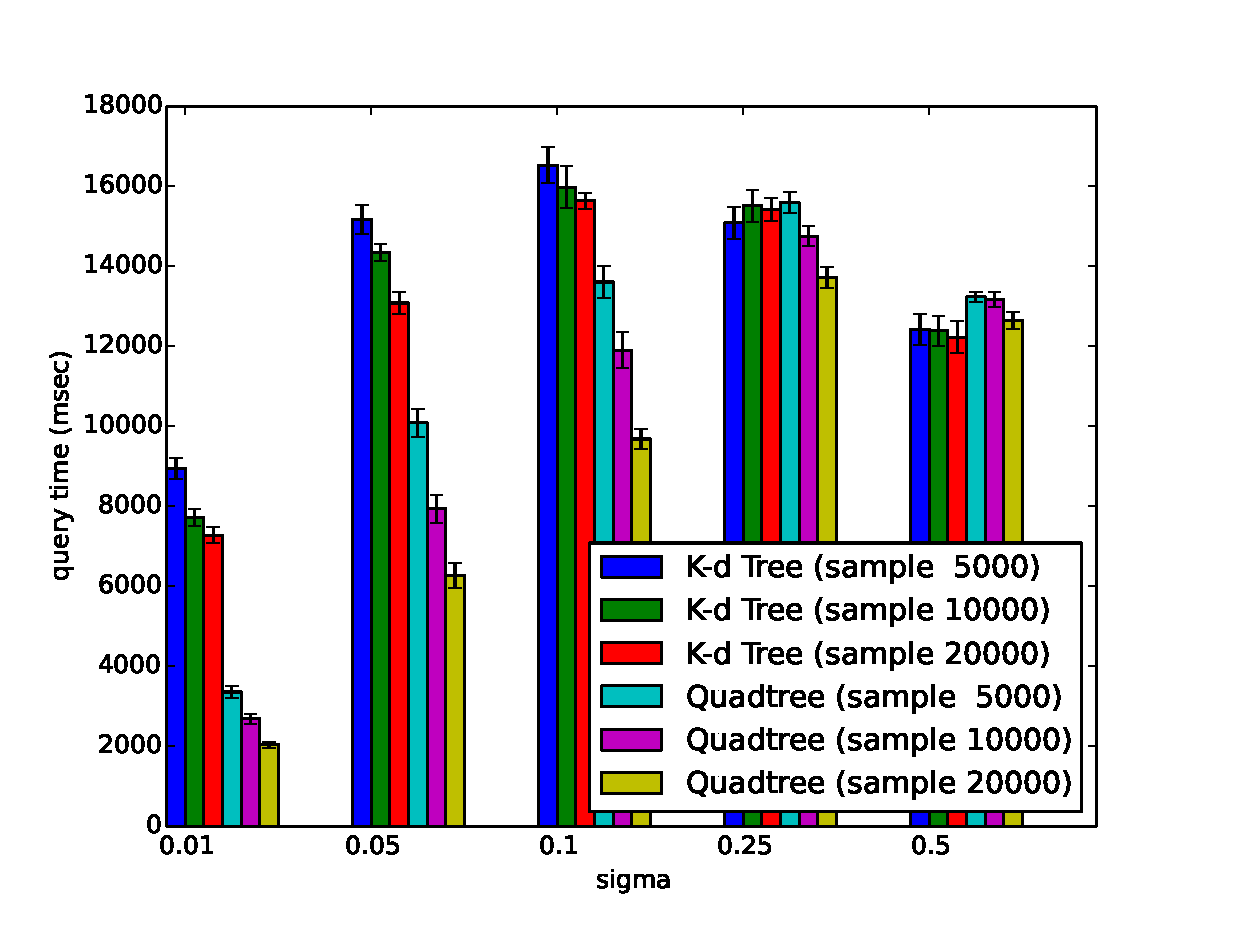
\includegraphics[scale=0.5]{diagrams/3d_qt_kt_pts10000_qtime.eps}
\caption{Query Time(3d, pts=10000)}
\label{fig:3d_kd_qt_qtime}
\end{center}
\end{figure}

Comparing total run times, the quadtree based implementation outperforms the
kd-tree based implementation for low entropy conditions (sigma \(\le 0.05\))
figure ~\ref{fig:3d_kd_qt_total}. This is not the case in higher dimensions.
The quadtree based implementation is substantially worse than the kd-tree
base implementation for the \(d = 8\) case (see figure ~\ref{fig:8d_kd_qt_total}).
Quadtrees exhibit best performance in small dimensions. This is in part because
the number of child nodes of a quadtree node is \(2^d\) for a \(d\)-dimensional
quadtree.

The kd-tree based implementation does not perform well in higher dimensional
spaces either so the quadtree remains a viable implementation choice over the
dimensions for which the odds-on tree exhibits good performance.

\begin{figure}
\begin{center}
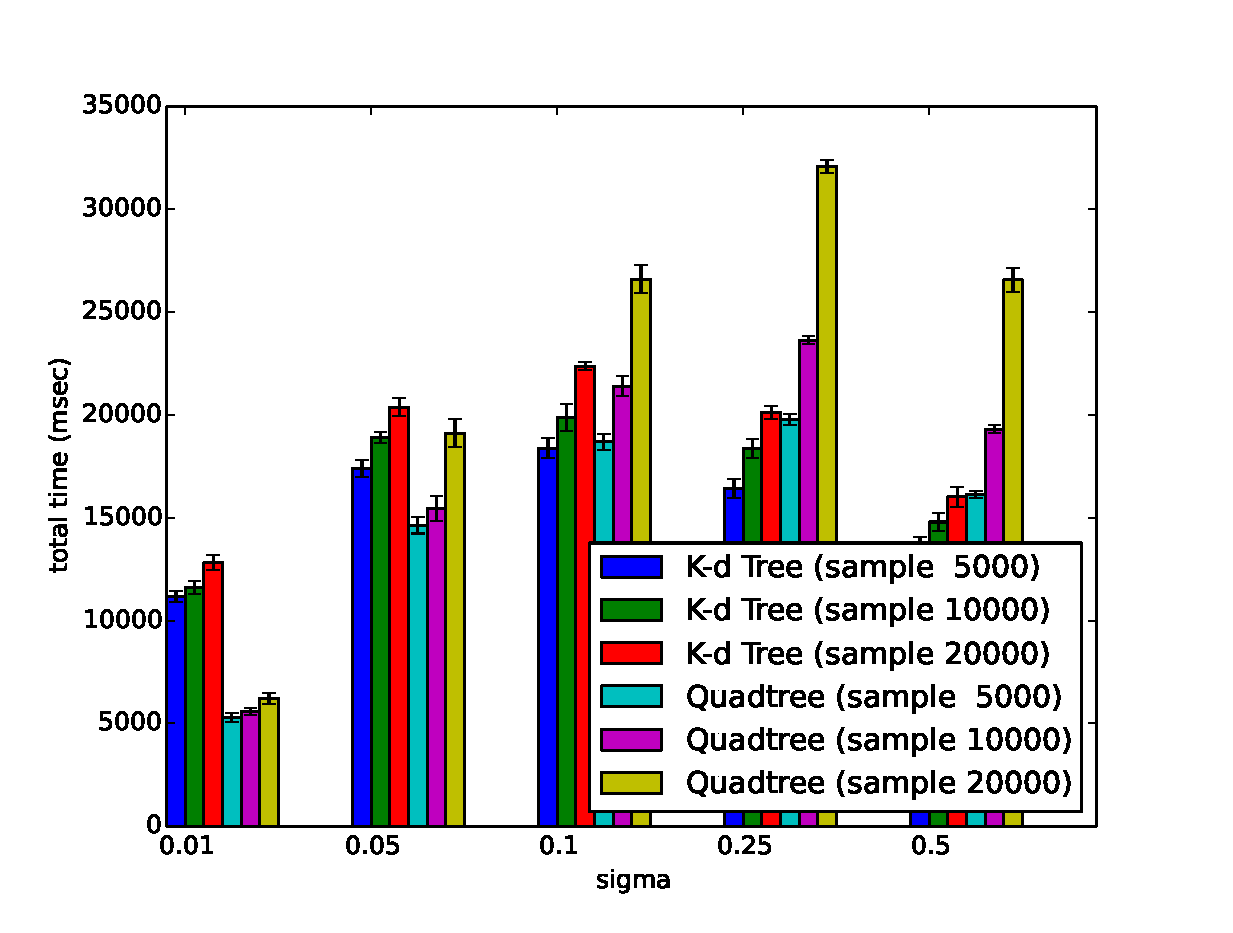
\includegraphics[scale=0.5]{diagrams/3d_qt_kt_pts10000_total.eps}
\caption{Total Time (3d, pts=10000)}
\label{fig:3d_kd_qt_total}
\end{center}
\end{figure}

\begin{figure}
\begin{center}
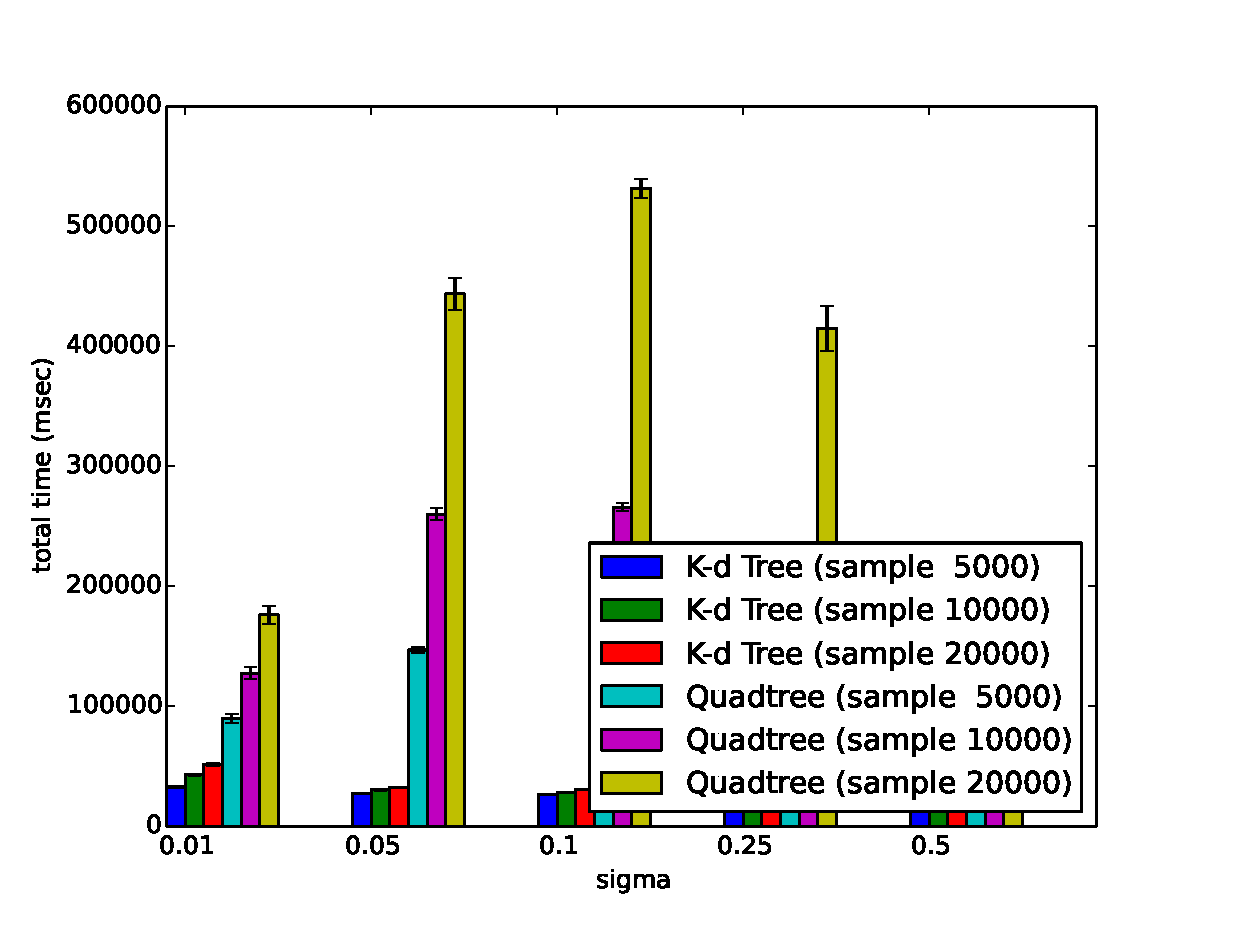
\includegraphics[scale=0.5]{diagrams/8d_qt_kt_pts10000_total.eps}
\caption{Total Time (8d, pts=10000)}
\label{fig:8d_kd_qt_total}
\end{center}
\end{figure}

Cache hit rate measures the number of times the odds-on tree is able to answer
a search without making use of the backup kd-tree structure. In general, the
quadtree has a better hit rate than the kd-tree based odds-on tree. Typical
results are shown in figure ~\ref{fig:2d_kd_qt_hits}.

\begin{figure}
\begin{center}
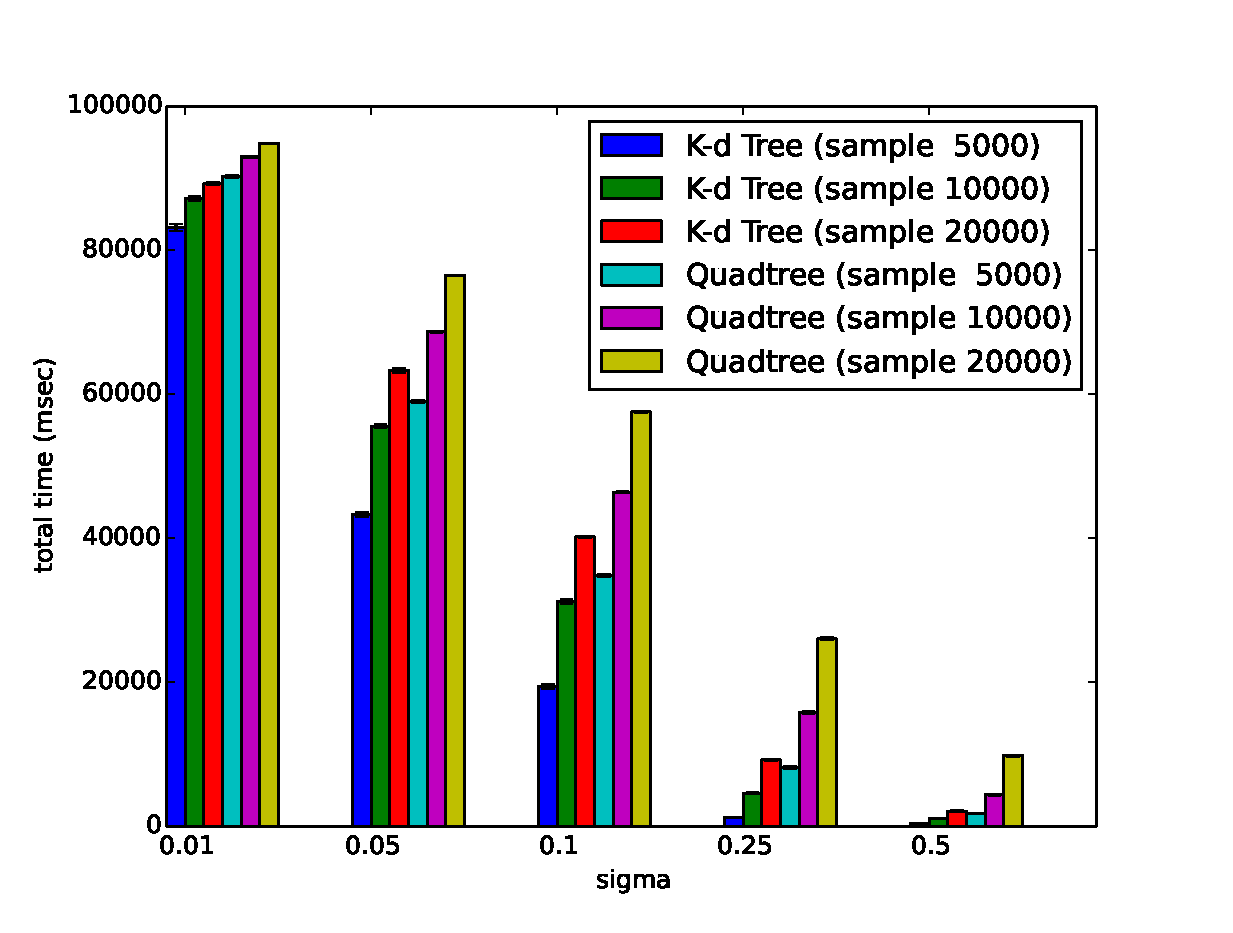
\includegraphics[scale=0.5]{diagrams/2d_qt_kt_pts10000_hits.eps}
\caption{Cache Hits (2d, pts=10000)}
\label{fig:2d_kd_qt_hits}
\end{center}
\end{figure}

For a node to be marked terminal the area it covers must have the same nearest
neighbour. Since the interference queries are run from the corners of the node,
a certain area outside of the node must also have the same nearest neighbour.
A square node requires less area outside of the node to have the same nearest
neighbour and so is more likely to be marked terminal. The area that must have
the same nearest neighbour for a square and for a rectangular node is
illustrated in figure ~\ref{fig:node_coverage}.

A quadtree node always has equal length sides, but a kd-tree node is built
by sub-dividing points and may have some sides much longer than others. Because
of this, given a quadtree node and a kd-tree node of the same area the kd-tree
node is less likely to be marked terminal, which means that a kd-tree based
odds-on tree implementation is likely to have a greater number of smaller nodes,
which will cause a lower cache hit rate.

\begin{figure}
\begin{center}
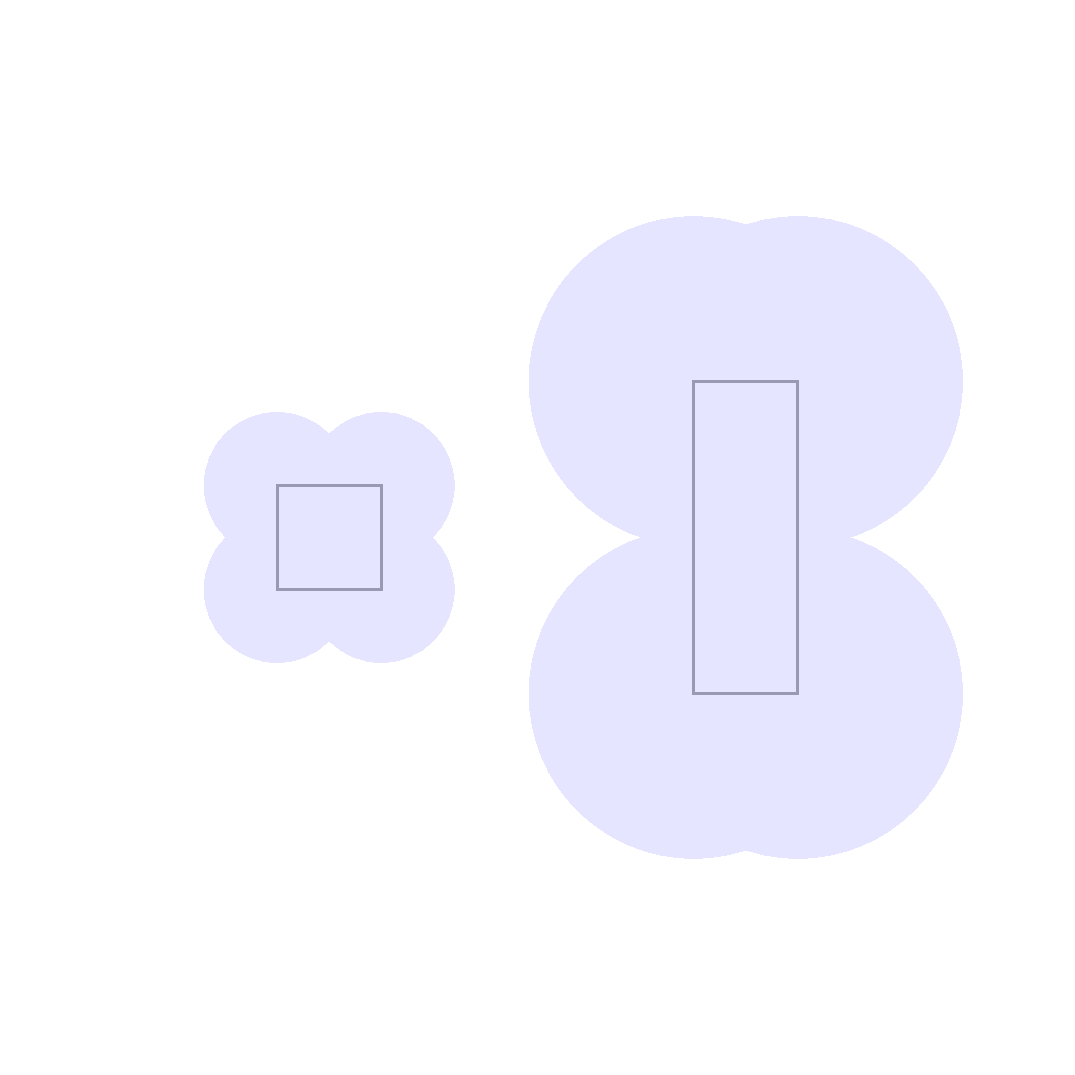
\includegraphics[scale=0.5]{diagrams/node_coverage.eps}
\caption{Square vs Rectangular Nodes}
\label{fig:node_coverage}
\end{center}
\end{figure}

The quadtree based implementation is able to build a more efficient cache than
the kd-tree based implementation. Because of this, it exhibits better
performance than the kd-tree based implementations for small values of search
set sigma.

\chapter{Conclusions}

\section{Summary}

We have shown in this thesis that it is possible to create a practical data
structure for biased neighbour search based upon odds-on trees. We developed
implementations based upon quadtrees and kd-trees and through a series of
careful experiments, compared their performance to our kd-tree implementation,
on a number of synthetic datasets.

Our primary metric was running time but we also considered cache hit ratios,
when comparing performance between odds-on tree implementations.

We found both implementations would outperform the kd-tree provided the entropy
of the set of sites returned under the search distribution is sufficiently
small. For small dimensions and sufficiently low search entropy, we found that
the quadtree will outperform the kd-tree based implementation. For large
dimensions, neither implementation performed bettered than a kd-tree.

Increasing the number of samples used to build the odds-on tree increased
build time but resulted in building a better cache. Adjusting the maximum
build depth did not have a clear effect on the build times or the quality of the
cache. Increasing the point set size did not change the relative performance
of the implementations.

\section{Future Work}

The experimentation in this thesis focused on synthetic datasets due to the
difficulty in finding ``real world'' datasets that included search distributions
as well as the underlying point sets. Further experimentation should be done
if suitable non-synthetic datasets are found.

The quadtree based implementation outperformed the kd-tree based implementation
in some cases due to creating nodes that have equal side length. Our kd-tree
implementation followed the original strategy in \cite{kdtree} of sorting the
points into two equal sized groups. In applications of kd-trees, particularly
in graphics, a number of other heuristic approaches have been developed that 
attempt to avoid creating nodes with a great disparity in side length
\cite{physicallybasedrendering}. Using these heuristics might provide better
performance than either a quadtree or a standard kd-tree.

The Balanced Box Decomposition (BBD) Tree \cite{optimalann} is a more
complicated data structure that maintains the equal space and equal partition
size properties of quadtrees and kd-trees. It was not implemented as part of
this thesis as its reported performance in the literature did not seem to
justify dealing with the increased complexity of implementation. Given the
results found that quadtrees build better caches than kd-trees it now seems
worthwhile implementing.

This thesis did not investigate the k nearest neighbour problem, where rather
than returning a single nearest neighbour instead k nearest neighbours are
returned. Intuitively, increasing k should have a negative impact on the cache
as the area covered by a node that has the same k nearest neighbours will be
smaller than the area covered by a node with only a single nearest neighbour.
This could be investigated experimentally.

A large portion of the time in doing a k-nearest neighbour search is spent in
backtracking, where other potential nearest neighbours are investigated after
the candidate nearest neighbours have been identified. The odds-on tree could
potentially be used to prune the number of nodes investigated during back
tracking, which might improve performance.

This thesis also did not investigate approximate nearest neighbour search. An
approximate nearest neighbour search often dramatically reduces the amount of
backtracking required to identify nearest neighbours and performs better in
higher dimensional spaces. The straightforward approach would be to mark nodes
as terminal that have the same approximate nearest neighbours.

Approximate Voronoi Diagrams \cite{avd} were not considered for implementation
in this thesis as they only work in the approximate case, but would be
worthwhile investigating in the future if further work were done with
approximate nearest neighour search.

\begin{thebibliography}{5}

\bibitem{treap}
Aragon, C. R.,  Seidel, R. (1996) Randomized Search Trees.
In Algorithmica, Vol. 16, Number 4/5, pp. 464 -- 497.

\bibitem{fastvector}
Arya, S., Mount, D. M. (1993) Algorithms for Fast Vector Quantization,
Proceedings of DCC '93, IEEE Press, pp 381 -- 390. 

\bibitem{app-ann}
Arya, S., Mount, D. M. (1993) Approximate nearest neighbour queries in Fixed
Dimensions, Proceedings of the 4th ACIM-SIAM Symposium on Discrete Algorithms,
pp 271 -- 280.

\bibitem{optimalann}
Arya, S., Mount, D. M., Netanyahu, N. S., Silverman, R. Wu, A. Y. (1998)
An Optimal Algorithm for Approximate Nearest Neighbor Searching in Fixed
Dimensions, Journal of the ACM, Volume 45, Issue 6, pp 891 -- 923.

\bibitem{simpleentropy}
Arya, S., Malamatos, T. Mount, D. M. (2001) A Simple Entropy-Based Algorithm
for Planar Point Location. In Proceedings of the Twelfth Annual ACM-SIAM
Symposium on Discrete Algorithms, pp. 262 -- 268.

\bibitem{arya-avd}
Arya, S., Malamatos, T. Mount, D. M. (2002) Space-efficient Approximate
Voronoi Diagrams, Proceedings of the 33rd Annual ACM Symposium on the Theory
of Computing, pp. 721 -- 730.

\bibitem{bsl}
Bagchi, A. Buchsbaum, A. L., Goodrich, M. T. (2005) Biased Skip Lists.
In Algorithmica Vol. 42, pp. 31 -- 48.

\bibitem{bst}
Bent, S. W., Sleator, D. D., Tarjan, R. E. (1984) Biased Search Trees,
In SIAM Journal on Computing, Volume 14, pp. 545 -- 568.

\bibitem{kdtree}
Bentley, J. L. (1975) Multidimensional Binary Search Trees Used for Associative
Searching, In Communications of the ACM, Volume 18, Number 9, pp. 509 -- 517.

\bibitem{rangetree}
Bentley, J. L. (1980) Multidimensional Divide-and-Conquer.
In Communications of the ACM, Volume 23, pp. 214 -- 229.

\bibitem{bern}
Bern, M., Eppstein, D., Teng, S-H. (1993) Parallel Construction of Quadtrees and
Quality Triangulations, WADS '93: Proceedings of the Third Workshop on
Algorithms and Data Structures, pp. 188 -- 199. 

\bibitem{oddson}
Bose, P., Devroye, L, Douieb, K., Dujmovic, V., King, J., Morin, P. (2010)
Odds-On Trees, preprint, retrieved from http://arxiv.org/abs/1002.1092 on
April 27, 2013.

\bibitem{chan}
Chan, T. M. (2006) A Minimalist's Implementation of an Approximate Nearest
Neighbour Algorithm in Fixed Dimensions, unpublished note, retrieved from
\url{http://www.cs.uwaterloo.ca/~tmchan/pub\_ann.html} on July 29, 2012.

\bibitem{chazelle} Chazelle, B. (1993) Cutting hyperplanes for divide-and-conquer.
Discrete and Computational Geometry 9, pp. 145 -- 158.

\bibitem{compressedquadtree}
Clarkson, Kenneth L. (1983) Fast Algorithms for the All Nearest Neighbors Problem,
FOCS '83: Proceedings of the Twenty-fourth Symposium on Foundations of
Computer Science, Tucson, AZ. 

\bibitem{connor}
Connor, M. and Kumar, P. (2009) Fast Construction of k-Nearest Neighbor Graphs
For Point Clouds, IEEE Transactions of Visualization and Computer Graphics,
September 2009.

\bibitem{dutch}
de Berg., M. van Kreveld, M., Overmars, M., Schwarzkopf, O. (2000)
Computational Geometry: Algorithms and Applications, 2nd Edition, Springer-Verlag,
Berlin Heidelberg New York.

\bibitem{biasedrange}
Dujmovic, V., Howat, J., Morin, P. (2009) Biased Range Trees
In Proceedings of the twentieth Annual ACM-SIAM Symposium on Discrete Algorithms,
New York, New York, pp. 486 -- 495.

\bibitem{edelsbrunner}
Edelsbrunner, H., Guibas, L. J., Stolfi, J. (1986) Optimal Point Location in a
Monotone Subdivision, SIAM Journal on Computing, 15(2), pp. 317 -- 340. 

\bibitem{skipquadtree}
Eppstein, D., Goodrich, M. T., Sun, J. Z. (2008) The Skip Quadtree: A Simple
Dynamic Data Structure for Multidimensional Data, Int. Journal on Computational
Geometry and Applications, 18(1/2), pp. 131 -- 160.

\bibitem{bsl2}
Ergun, F., Sahinalp, S. C., Sharp, J., Sinha, R. K. (2001) Biased Skip Lists
for Highly Skewed Access Patterns, Proceedings of ALENEX 2001, Lecture Notes in
Computer Science, Volume 2153, pp. 216 -- 229.

\bibitem{bst2}
Feigenbaum, J., Tarjan, R. E. (1983) Two New Kinds of Biased Search Tree,
In Bell Systems Technical Journal, Vol. 62, No. 10, pp. 3139 -- 3158.

\bibitem{quadtree}
Finkel, R. A. and Bentley, J. L. (1974) Quad Trees A Data Structure for
Retrieval on Composite Keys, Acta Informatica, 4(1), pp. 1 –- 9.

\bibitem{friedman}
Friedman, J. H., Bentley, J. L., Finkel, R. A. (1977) An Algorithm for Finding
Best Matches in Logarithmic Expected Time, ACM Transactions on Mathematical
Software, Vol. 3 Number 3, pp. 209 -- 226.

\bibitem{rtree}
Guttman, A. (1984) R-Trees: A Dynamic Index Structure for Spatial Searching,
SIGMOD '84: Proceedings of the 1984 ACM SIGMOD International Conference on the
Management of Data, pp. 47 -- 58.

\bibitem{avd}
Har-Peled, S. (2001) A Replacement for Voronoi Diagrams of Near Linear Size, 
FOCS '01: Proceedings of the Symposium on Foundations of Computer Science, 
pp. 94 -- 103.

\bibitem{iacono}
Iacono, J. (2001) Optimal Planar Point Location
In Proceedings of the Twelfth Annual ACM-SIAM Symposium on Discrete Algorithms,
pp. 240 -- 241.

\bibitem{lsh}
Indyk, P., Motwani, R. (1998) Approximate Nearest Neighbors: Towards Removing
the Curse of Dimensionality, In Proceedings of the Thirtieth Annual ACM
Symposium on Theory of Computing, pp. 604 -- 613.

\bibitem{kirkpatrick}
Kirkpatrick, D. (1983) Optimal Search in Planar Subdivisions,
Siam Journal of Computing, Vol. 12, No. 1, pp. 28 -- 34.

\bibitem{knuth}
Knuth, D. E. (1998) The Art of Computer Programming, Second Edition,
Volume 3, Sorting and Searching. Addison-Wesley, Reading, Massachusetts, USA.

\bibitem{practicalann}
Liu, T., Moore, A. W., Gray, A., Yang, K. (2004) An Investigation of Practical
Approximate Nearest-Neighbour Algorithms, Proceedings of Neural Information
Processing Systems(NIPS 2004), pp. 825 -- 832.

\bibitem{mehlhorn}
Mehlhorn, K. (1975) Nearly Optimal Binary Search Trees 
In Acta Informatica, 5(1), pp. 287 -- 295.

\bibitem{frequency-english}
Mines, M. A., Hanson, B. F., Shoup, J. E. (1978) Frequency of Occurence of
Phonemes in Conversational English, Language and Speech, vol. 21 no. 3,
pp. 221 -- 241 

\bibitem{morton}
Morton, G. M. (1966), A Computer Oriented Geodetic Data Base; and a New
Technique in File Sequencing, Technical Report, IBM Ltd., Ottawa, Canada.

\bibitem{ann}
Mount, D. M., Arya, S. (2012) ANN: A Library for Approximate Nearest Neighbor
Searching, retrieved from \url{http://www.cs.umd.edu/~mount/ANN} on July 29, 2012.

\bibitem{physicallybasedrendering}
Pharr, M., Humphreys, G. (2010) Physically Based Rendering
Morgan-Kaufmann, San Francisco, CA.

\bibitem{skiplist}
Pugh, W. (1990) Skip Lists: A Probabilistic Alternative to Balanced Trees.
In Communications of the ACM, 33(6), pp. 668 -- 676.

\bibitem{rudin}
Rudin, W. (1976) Principles of Mathematical Analysis, Third Edition
McGraw-Hill, New York, NY.

\bibitem{samet}
Samet, H. (2006) Foundations of Multidimensional and Metric Data Structures
Morgan-Kaufmann, San Francisco, CA.

\bibitem{sarnak}
Sarnak, N. and Tarjan, R. E. (1986) Planar Point Location Using Persistent
Search Trees. Communications of the ACM, 29(7), pp. 669 -- 679.

\bibitem{shewchuk} Shewchuk, J. R. (2013) Lecture Notes on Geometric Robustness,
Retrieved from http://www.cs.berkeley.edu/~jrs/meshpapers/robnotes.pdf on
October 13, 2014.

\bibitem{claudeshannonwasagod}
Shannon, Claude E. (1948) A Mathematical Theory of Communication,
Bell System Technical Journal, 27, pp. 379 -- 423 and 623 -- 656.

\bibitem{splaytree}
Sleator, D. D., Tarjan, R. E. (1985) Self-adjusting binary search trees.
In Journal of the ACM, 32, pp. 652 -- 686.

\bibitem{yule}
Tambovtsev, Y. and Martindale, C. (2007) Phoneme Frequencies Follow a Yule
Distribution. SKASE Journal of Theoretical Linguistics 4: 2.

\bibitem{satp}
Williams, H. E., Zobel, J., Heinz, S. (2001) Self-Adjusting Trees in Practice
for Large Text Collections, In Software - Practice and Experience,
Volume 31, pp. 925 -- 939.

\end{thebibliography}

\end{document}
